\documentclass[a4paper,english,11pt]{article}\usepackage[]{graphicx}\usepackage[]{xcolor}
% maxwidth is the original width if it is less than linewidth
% otherwise use linewidth (to make sure the graphics do not exceed the margin)
\makeatletter
\def\maxwidth{ %
  \ifdim\Gin@nat@width>\linewidth
    \linewidth
  \else
    \Gin@nat@width
  \fi
}
\makeatother

\definecolor{fgcolor}{rgb}{0.345, 0.345, 0.345}
\newcommand{\hlnum}[1]{\textcolor[rgb]{0.686,0.059,0.569}{#1}}%
\newcommand{\hlsng}[1]{\textcolor[rgb]{0.192,0.494,0.8}{#1}}%
\newcommand{\hlcom}[1]{\textcolor[rgb]{0.678,0.584,0.686}{\textit{#1}}}%
\newcommand{\hlopt}[1]{\textcolor[rgb]{0,0,0}{#1}}%
\newcommand{\hldef}[1]{\textcolor[rgb]{0.345,0.345,0.345}{#1}}%
\newcommand{\hlkwa}[1]{\textcolor[rgb]{0.161,0.373,0.58}{\textbf{#1}}}%
\newcommand{\hlkwb}[1]{\textcolor[rgb]{0.69,0.353,0.396}{#1}}%
\newcommand{\hlkwc}[1]{\textcolor[rgb]{0.333,0.667,0.333}{#1}}%
\newcommand{\hlkwd}[1]{\textcolor[rgb]{0.737,0.353,0.396}{\textbf{#1}}}%
\let\hlipl\hlkwb

\usepackage{framed}
\makeatletter
\newenvironment{kframe}{%
 \def\at@end@of@kframe{}%
 \ifinner\ifhmode%
  \def\at@end@of@kframe{\end{minipage}}%
  \begin{minipage}{\columnwidth}%
 \fi\fi%
 \def\FrameCommand##1{\hskip\@totalleftmargin \hskip-\fboxsep
 \colorbox{shadecolor}{##1}\hskip-\fboxsep
     % There is no \\@totalrightmargin, so:
     \hskip-\linewidth \hskip-\@totalleftmargin \hskip\columnwidth}%
 \MakeFramed {\advance\hsize-\width
   \@totalleftmargin\z@ \linewidth\hsize
   \@setminipage}}%
 {\par\unskip\endMakeFramed%
 \at@end@of@kframe}
\makeatother

\definecolor{shadecolor}{rgb}{.97, .97, .97}
\definecolor{messagecolor}{rgb}{0, 0, 0}
\definecolor{warningcolor}{rgb}{1, 0, 1}
\definecolor{errorcolor}{rgb}{1, 0, 0}
\newenvironment{knitrout}{}{} % an empty environment to be redefined in TeX

\usepackage{alltt}
\usepackage{a4a}
\IfFileExists{upquote.sty}{\usepackage{upquote}}{}
\begin{document}

\title{Step by step demo for the \aFa statistical catch-at-age framework}

\author[1]{Ernesto Jardim}
\author[1,2,3]{Colin Millar}
\affil[1]{European Commission, Joint Research Centre, Sustainable resources directorate, Water and Marine Resources unit, 21027 Ispra (VA), Italy}
\affil[3]{International Council for the Exploration of the Sea (ICES), H. C. Andersens Boulevard 44-46, 1553 Copenhagen V, Denmark}
\affil[*]{Corresponding author \href{mailto:ernesto.jardim@ec.europa.eu}{ernesto.jardim@ec.europa.eu}}


\maketitle

\begin{abstract}
%This chapter presents the statistical catch-at-age stock assessment model developed as part of the Assessment For All (\aFa) initiative of the European Commission Joint Research Centre. The stock assessment model framework is a non-linear catch-at-age model implemented in \href{http://www.r-project.org/}{\R}, \href{http://www.flr-project.org/}{\FLR} and \href{http://www.admb-project.org/}{\ADMB}, that can be applied rapidly to a wide range of situations with low parametrization requirements. The model structure is defined by submodels, which are the different parts that require structural assumptions. There are 5 submodels in operation: F-at-age, abundance indices catchability-at-age, recruitment, observation variance of catch-at-age and abundance indices-at-age, and population's age structurein the first year. All submodels use the same type of specification process, the \R formula interface, wich gives lot's of flexibility to explore models and combination of submodels.
\end{abstract}

\newpage
\tableofcontents
\newpage



\section{Before starting}

\subsection{License, documentation and development status}

The software is released under the \href{https://joinup.ec.europa.eu/community/eupl/home}{EUPL 1.1}.

For more information on the \aFa methodologies refer to \href{http://icesjms.oxfordjournals.org/content/early/2014/04/03/icesjms.fsu050.abstract}{Jardim, et.al, 2014}, \href{http://icesjms.oxfordjournals.org/content/early/2014/03/31/icesjms.fsu043.abstract}{Millar, et.al, 2014} and \href{http://journals.plos.org/plosone/article?id=10.1371/journal.pone.0154922}{Scott, et.al, 2016}.

Documentation can be found at \url{http://flr-project.org/FLa4a}. You are welcome to:

\begin{itemize}
	\item Submit suggestions and bug-reports at: \url{https://github.com/flr/FLa4a/issues}
	\item Send a pull request on: \url{https://github.com/flr/FLa4a/}
	\item Compose a friendly e-mail to the maintainer, see `packageDescription('FLa4a')`
\end{itemize}

\subsection{Installing and loading libraries}

To run the \code{FLa4a} methods the reader will need to install the package and its dependencies and load them. Some datasets are distributed with the package and as such need to be loaded too.

\begin{knitrout}
\definecolor{shadecolor}{rgb}{0.949, 0.949, 0.949}\color{fgcolor}\begin{kframe}
\begin{alltt}
\hlcom{# from CRAN}
\hlkwd{install.packages}\hldef{(}\hlkwd{c}\hldef{(}\hlsng{"copula"}\hldef{,} \hlsng{"triangle"}\hldef{,} \hlsng{"coda"}\hldef{,} \hlsng{"grid"}\hldef{,} \hlsng{"gridExtra"}\hldef{,} \hlsng{"latticeExtra"}\hldef{))}
\hlcom{# from FLR}
\hlkwd{install.packages}\hldef{(}\hlkwd{c}\hldef{(}\hlsng{"FLCore"}\hldef{,} \hlsng{"FLa4a"}\hldef{),} \hlkwc{repos} \hldef{=} \hlsng{"http://flr-project.org/R"}\hldef{)}
\end{alltt}
\end{kframe}
\end{knitrout}

\begin{knitrout}
\definecolor{shadecolor}{rgb}{0.949, 0.949, 0.949}\color{fgcolor}\begin{kframe}
\begin{alltt}
\hlcom{# libraries}
\hlkwd{library}\hldef{(devtools)}
\hlkwd{library}\hldef{(FLa4a)}
\hlkwd{library}\hldef{(XML)}
\hlkwd{library}\hldef{(reshape2)}
\hlkwd{library}\hldef{(ggplotFL)}
\hlcom{# datasets}
\hlkwd{data}\hldef{(hke1567)}
\hlkwd{data}\hldef{(hke1567.idx)}
\end{alltt}
\end{kframe}
\end{knitrout}

\begin{knitrout}
\definecolor{shadecolor}{rgb}{0.949, 0.949, 0.949}\color{fgcolor}\begin{kframe}
\begin{alltt}
\hlkwd{packageVersion}\hldef{(}\hlsng{"FLCore"}\hldef{)}
\end{alltt}
\begin{verbatim}
## [1] '2.6.20.920'
\end{verbatim}
\begin{alltt}
\hlkwd{packageVersion}\hldef{(}\hlsng{"FLa4a"}\hldef{)}
\end{alltt}
\begin{verbatim}
## [1] '1.9.0'
\end{verbatim}
\end{kframe}
\end{knitrout}

\subsection{How to read this document}

The target audience for this document are readers with some experience in R and some background on stock assessment.

The document explains the approach being developed by \aFa for fish stock assessment and scientific advice. It presents a mixture of text and code, where the first explains the concepts behind the methods, while the last shows how these can be run with the software provided. Moreover, having the code allows the reader to copy/paste and replicate the analysis presented here.

The sections and subsections are as independent as possible, so it can be used as a reference document for the \code{FLa4a}. 

\section{Step by step}

\subsection{The "mean" model}

To start the analysis we'll fit a "mean" model, where all submodels will be set to an overall average, by using the \code{~1} formula. This will be our reference model to see how adding age and year effects will show up in the diagnostic tools, in particular in the residuals.

\begin{knitrout}
\definecolor{shadecolor}{rgb}{0.949, 0.949, 0.949}\color{fgcolor}\begin{kframe}
\begin{alltt}
\hldef{fit01} \hlkwb{<-} \hlkwd{sca}\hldef{(hke1567, hke1567.idx,} \hlkwc{fmod} \hldef{=} \hlopt{~}\hlnum{1}\hldef{,} \hlkwc{qmod} \hldef{=} \hlkwd{list}\hldef{(}\hlopt{~}\hlnum{1}\hldef{),} \hlkwc{srmod} \hldef{=} \hlopt{~}\hlnum{1}\hldef{,} \hlkwc{vmod} \hldef{=} \hlkwd{list}\hldef{(}\hlopt{~}\hlnum{1}\hldef{,}
    \hlopt{~}\hlnum{1}\hldef{),} \hlkwc{n1mod} \hldef{=} \hlopt{~}\hlnum{1}\hldef{)}
\hldef{res01} \hlkwb{<-} \hlkwd{residuals}\hldef{(fit01, hke1567, hke1567.idx)}
\end{alltt}
\end{kframe}
\end{knitrout}

The common residuals plot  clearly shows a trend across ages (figure~\ref{fig:meanresbyage}) for both datasets. 

\begin{knitrout}
\definecolor{shadecolor}{rgb}{0.949, 0.949, 0.949}\color{fgcolor}\begin{kframe}
\begin{alltt}
\hlkwd{plot}\hldef{(res01)}
\end{alltt}
\end{kframe}\begin{figure}[H]

{\centering 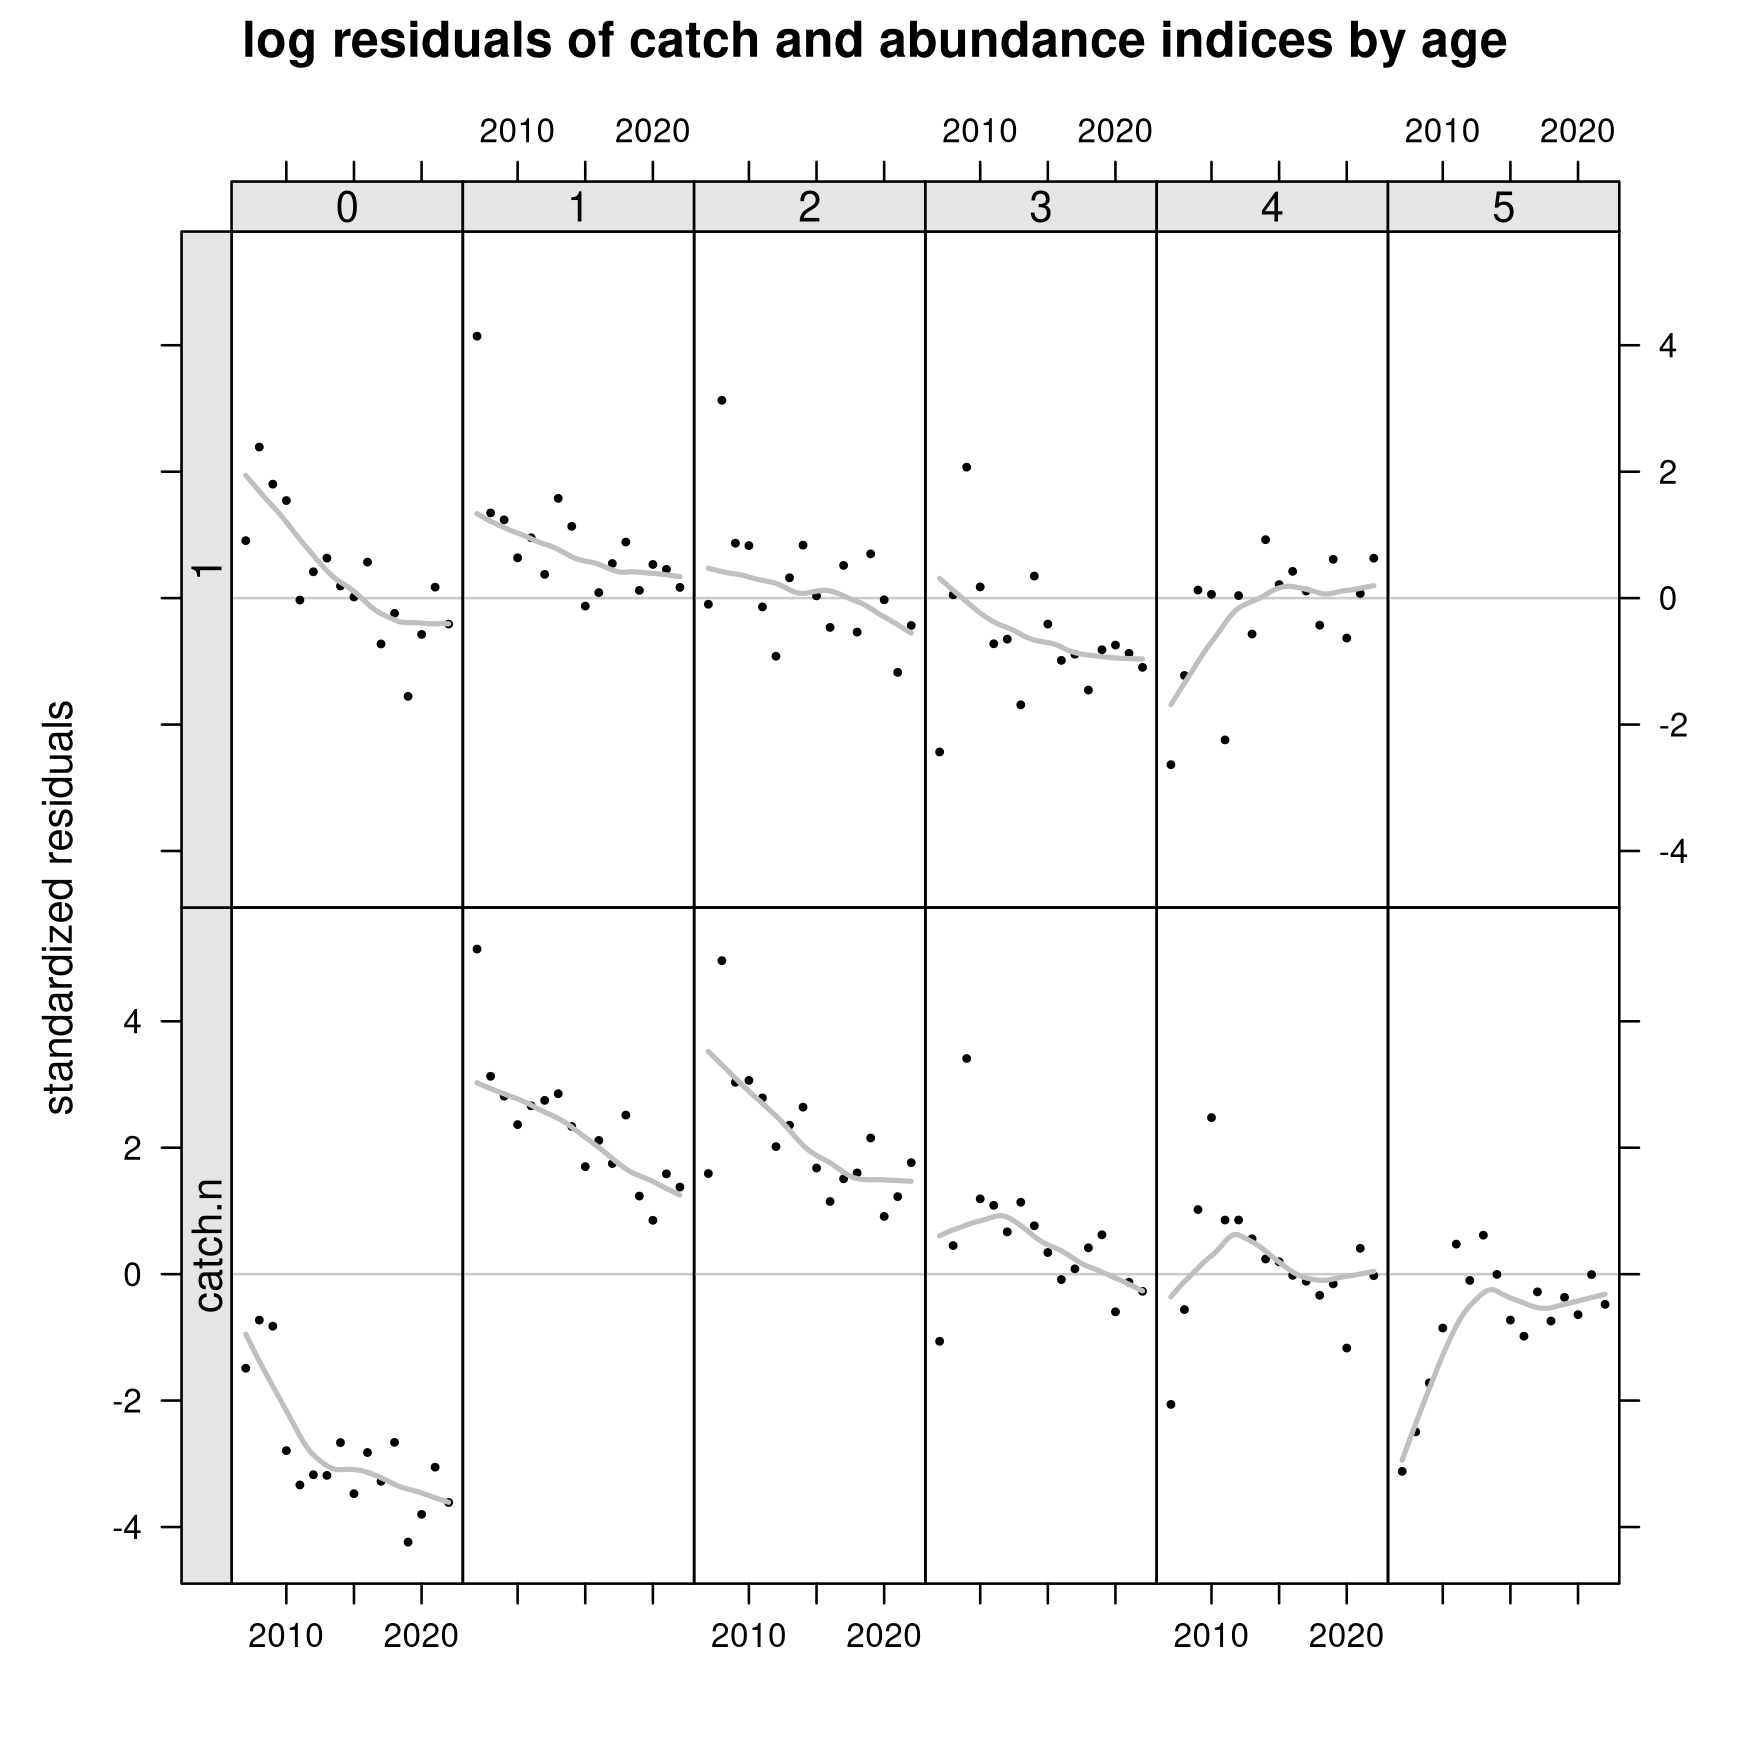
\includegraphics[width=.9\linewidth]{figure/meanresbyyear-1} 

}

\caption[Mean fit residuals by year)]{Mean fit residuals by year)}\label{fig:meanresbyyear}
\end{figure}

\end{knitrout}

Which is even clearer when plotting the residuals by age across years.

\begin{knitrout}
\definecolor{shadecolor}{rgb}{0.949, 0.949, 0.949}\color{fgcolor}\begin{kframe}
\begin{alltt}
\hlkwd{plot}\hldef{(res01,} \hlkwc{auxline} \hldef{=} \hlsng{"l"}\hldef{,} \hlkwc{by} \hldef{=} \hlsng{"age"}\hldef{)}
\end{alltt}
\end{kframe}\begin{figure}[H]

{\centering 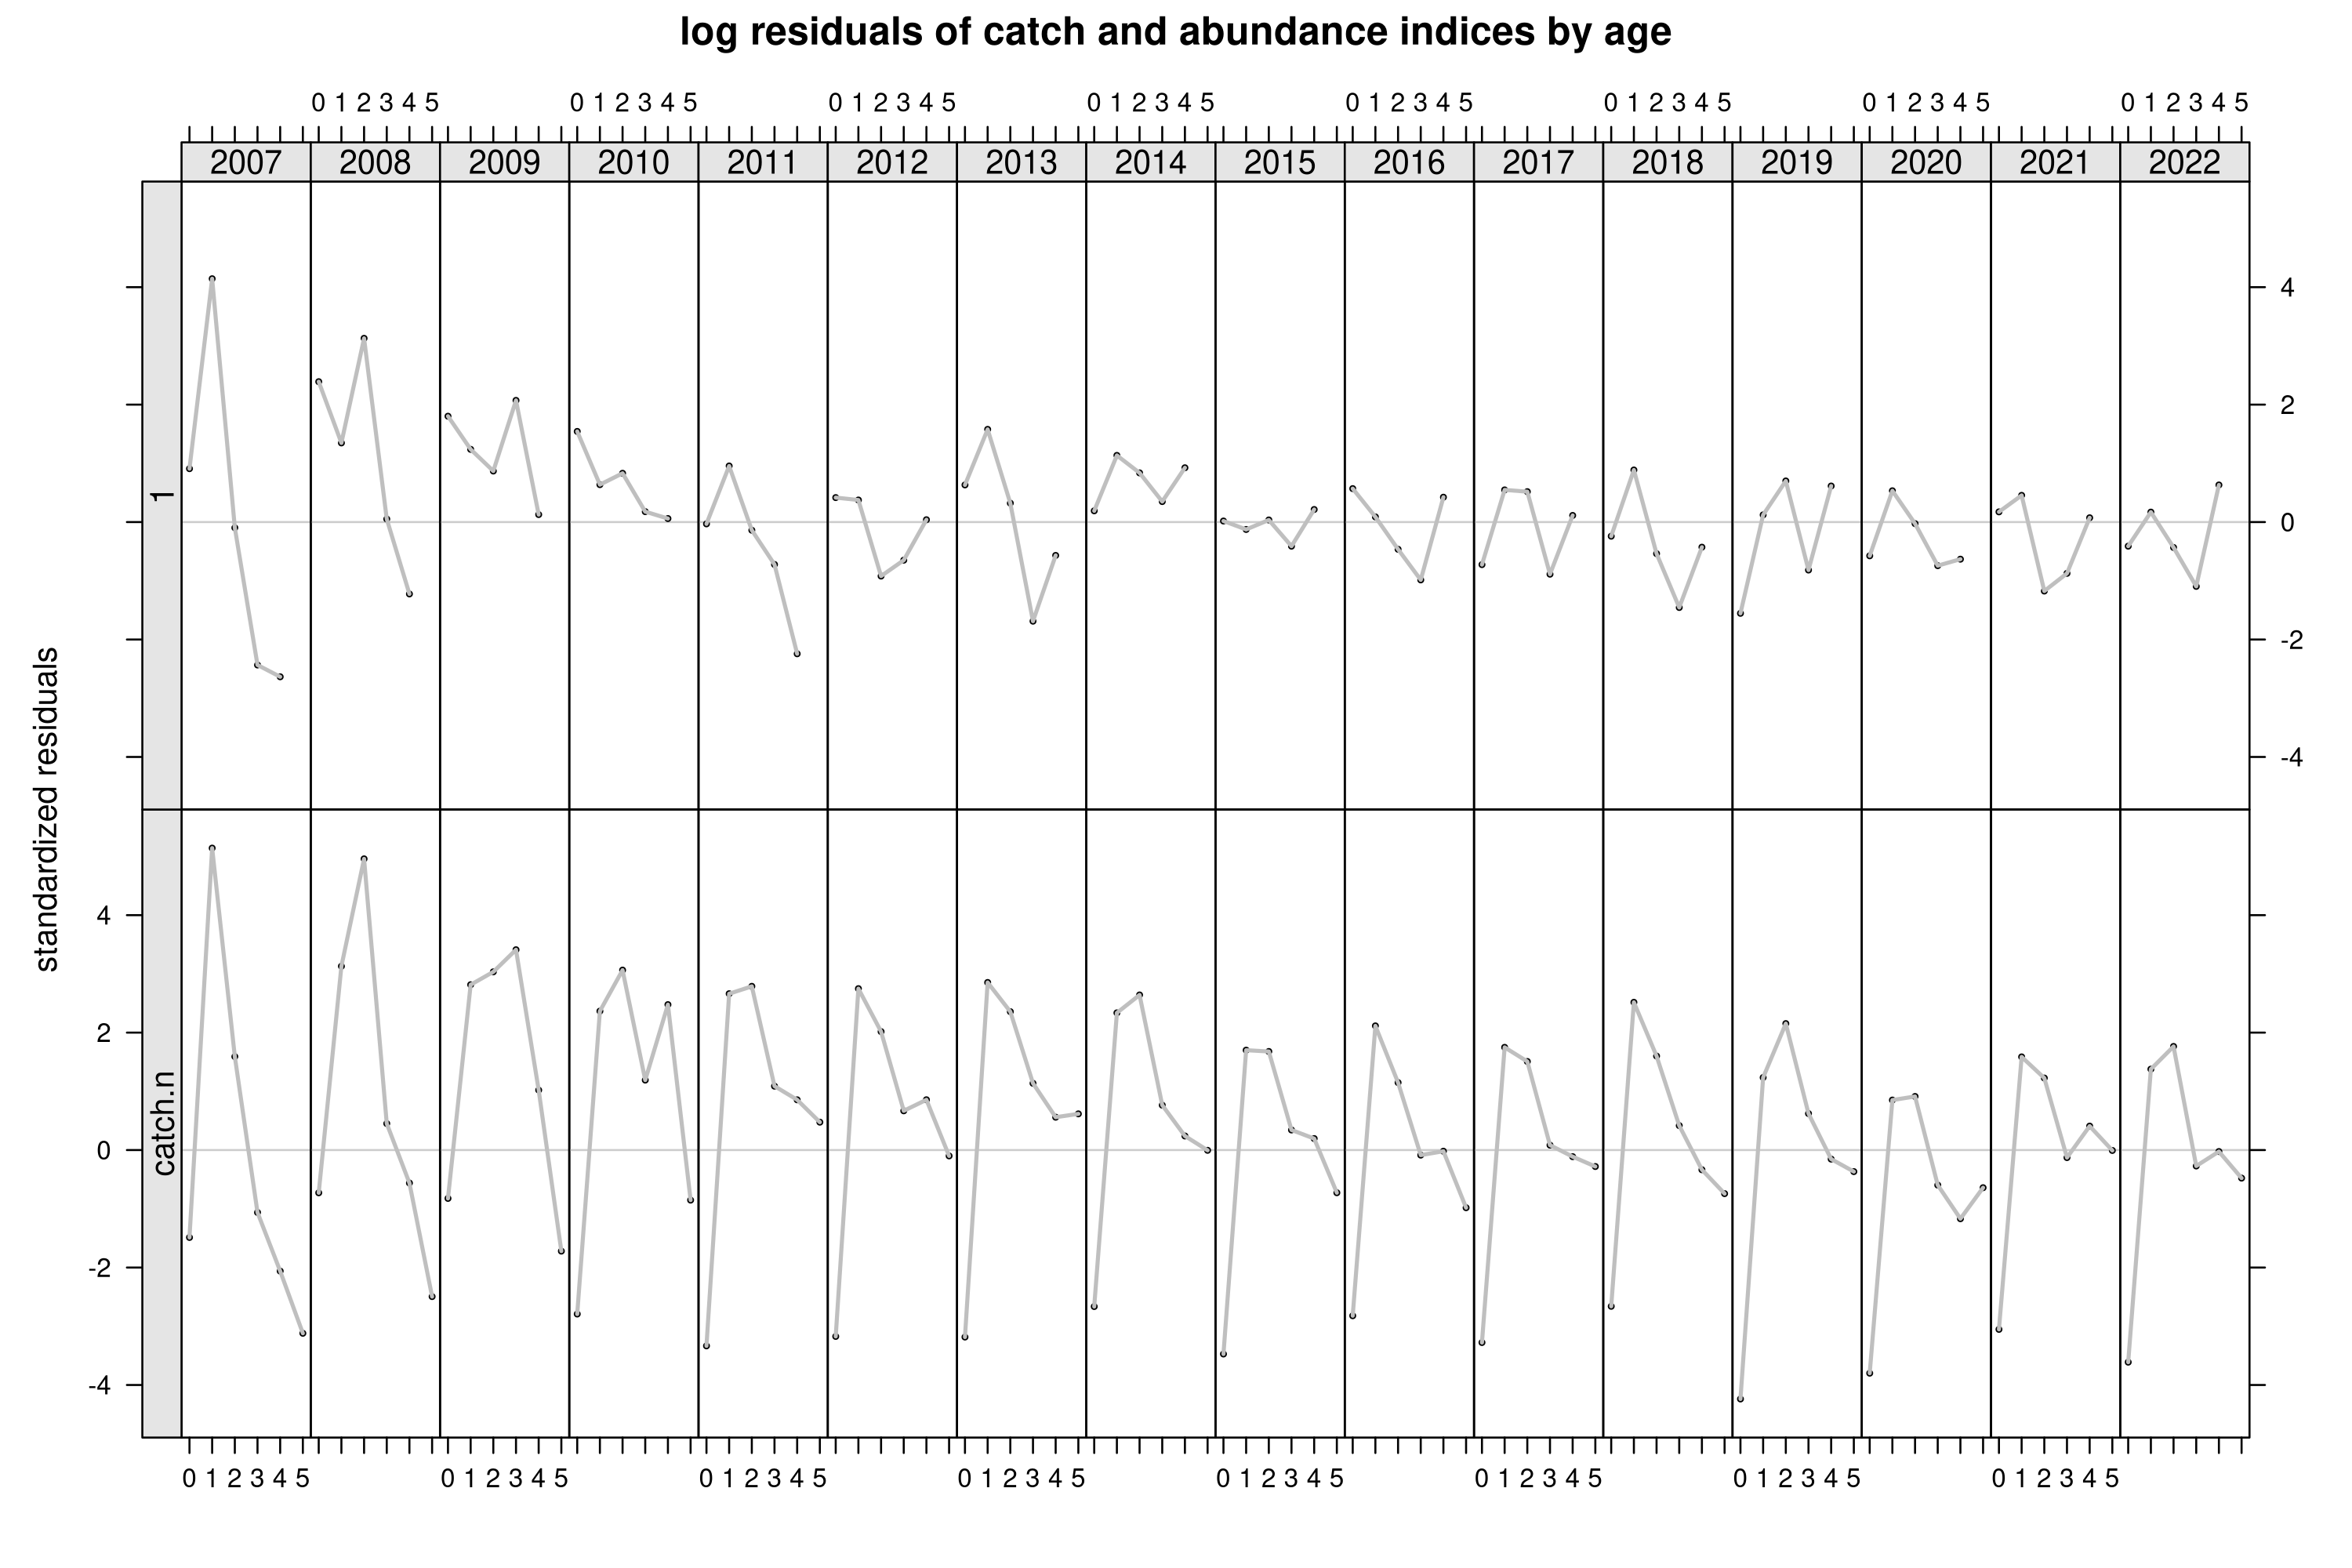
\includegraphics[width=25cm,height=18cm,angle=90]{figure/meanresbyage-1} 

}

\caption[Mean fit residuals by age)]{Mean fit residuals by age)}\label{fig:meanresbyage}
\end{figure}

\end{knitrout}

\subsection{The age effects}

These models will introduce age effects in the fishing mortality submodel and catchability submodel. First in the fishinf mortality submodel.

\begin{knitrout}
\definecolor{shadecolor}{rgb}{0.949, 0.949, 0.949}\color{fgcolor}\begin{kframe}
\begin{alltt}
\hldef{fit02} \hlkwb{<-} \hlkwd{sca}\hldef{(hke1567, hke1567.idx,} \hlkwc{fmod} \hldef{=} \hlopt{~}\hlkwd{factor}\hldef{(age),} \hlkwc{qmod} \hldef{=} \hlkwd{list}\hldef{(}\hlopt{~}\hlnum{1}\hldef{),} \hlkwc{srmod} \hldef{=} \hlopt{~}\hlnum{1}\hldef{,}
    \hlkwc{vmod} \hldef{=} \hlkwd{list}\hldef{(}\hlopt{~}\hlnum{1}\hldef{,} \hlopt{~}\hlnum{1}\hldef{),} \hlkwc{n1mod} \hldef{=} \hlopt{~}\hlnum{1}\hldef{)}
\hldef{res02} \hlkwb{<-} \hlkwd{residuals}\hldef{(fit02, hke1567, hke1567.idx)}
\end{alltt}
\end{kframe}
\end{knitrout}

The residuals plot now shows catch at age residuals less stagered, reflecting the modelling of the age effect. 

\begin{knitrout}
\definecolor{shadecolor}{rgb}{0.949, 0.949, 0.949}\color{fgcolor}\begin{kframe}
\begin{alltt}
\hlkwd{plot}\hldef{(res02)}
\end{alltt}
\end{kframe}\begin{figure}[H]

{\centering 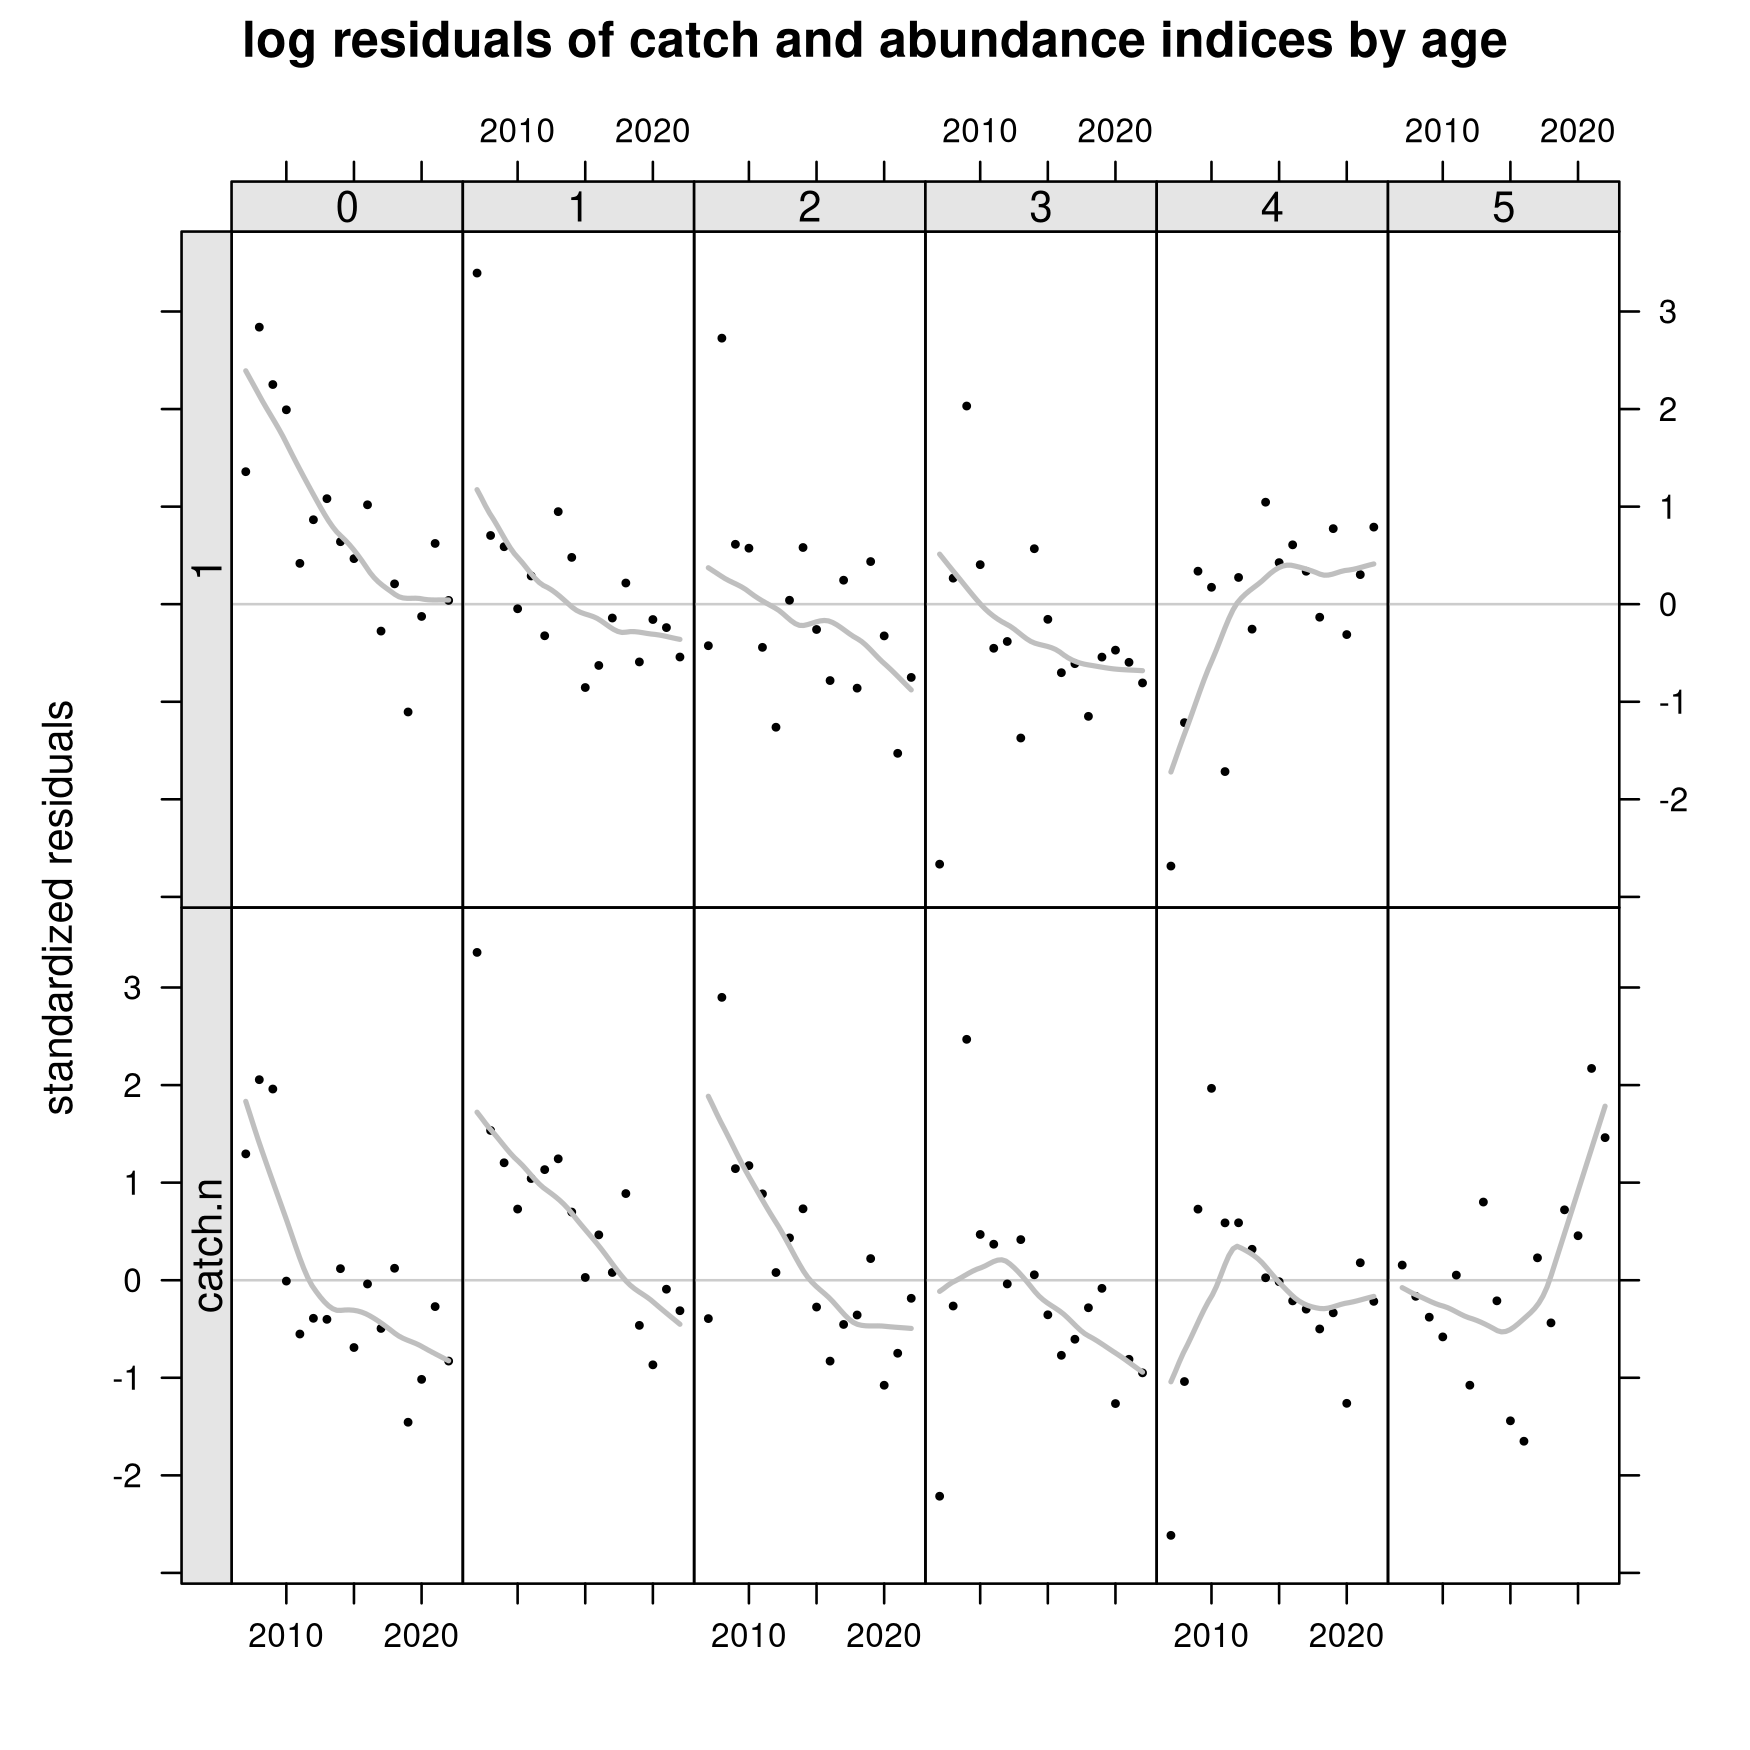
\includegraphics[width=.9\linewidth]{figure/fageresbyyear-1} 

}

\caption[f age effect fit residuals by year)]{f age effect fit residuals by year)}\label{fig:fageresbyyear}
\end{figure}

\end{knitrout}

The residuals plot by age shows the same outcome.  

\begin{knitrout}
\definecolor{shadecolor}{rgb}{0.949, 0.949, 0.949}\color{fgcolor}\begin{kframe}
\begin{alltt}
\hlkwd{plot}\hldef{(res02,} \hlkwc{auxline} \hldef{=} \hlsng{"l"}\hldef{,} \hlkwc{by} \hldef{=} \hlsng{"age"}\hldef{)}
\end{alltt}
\end{kframe}\begin{figure}[H]

{\centering 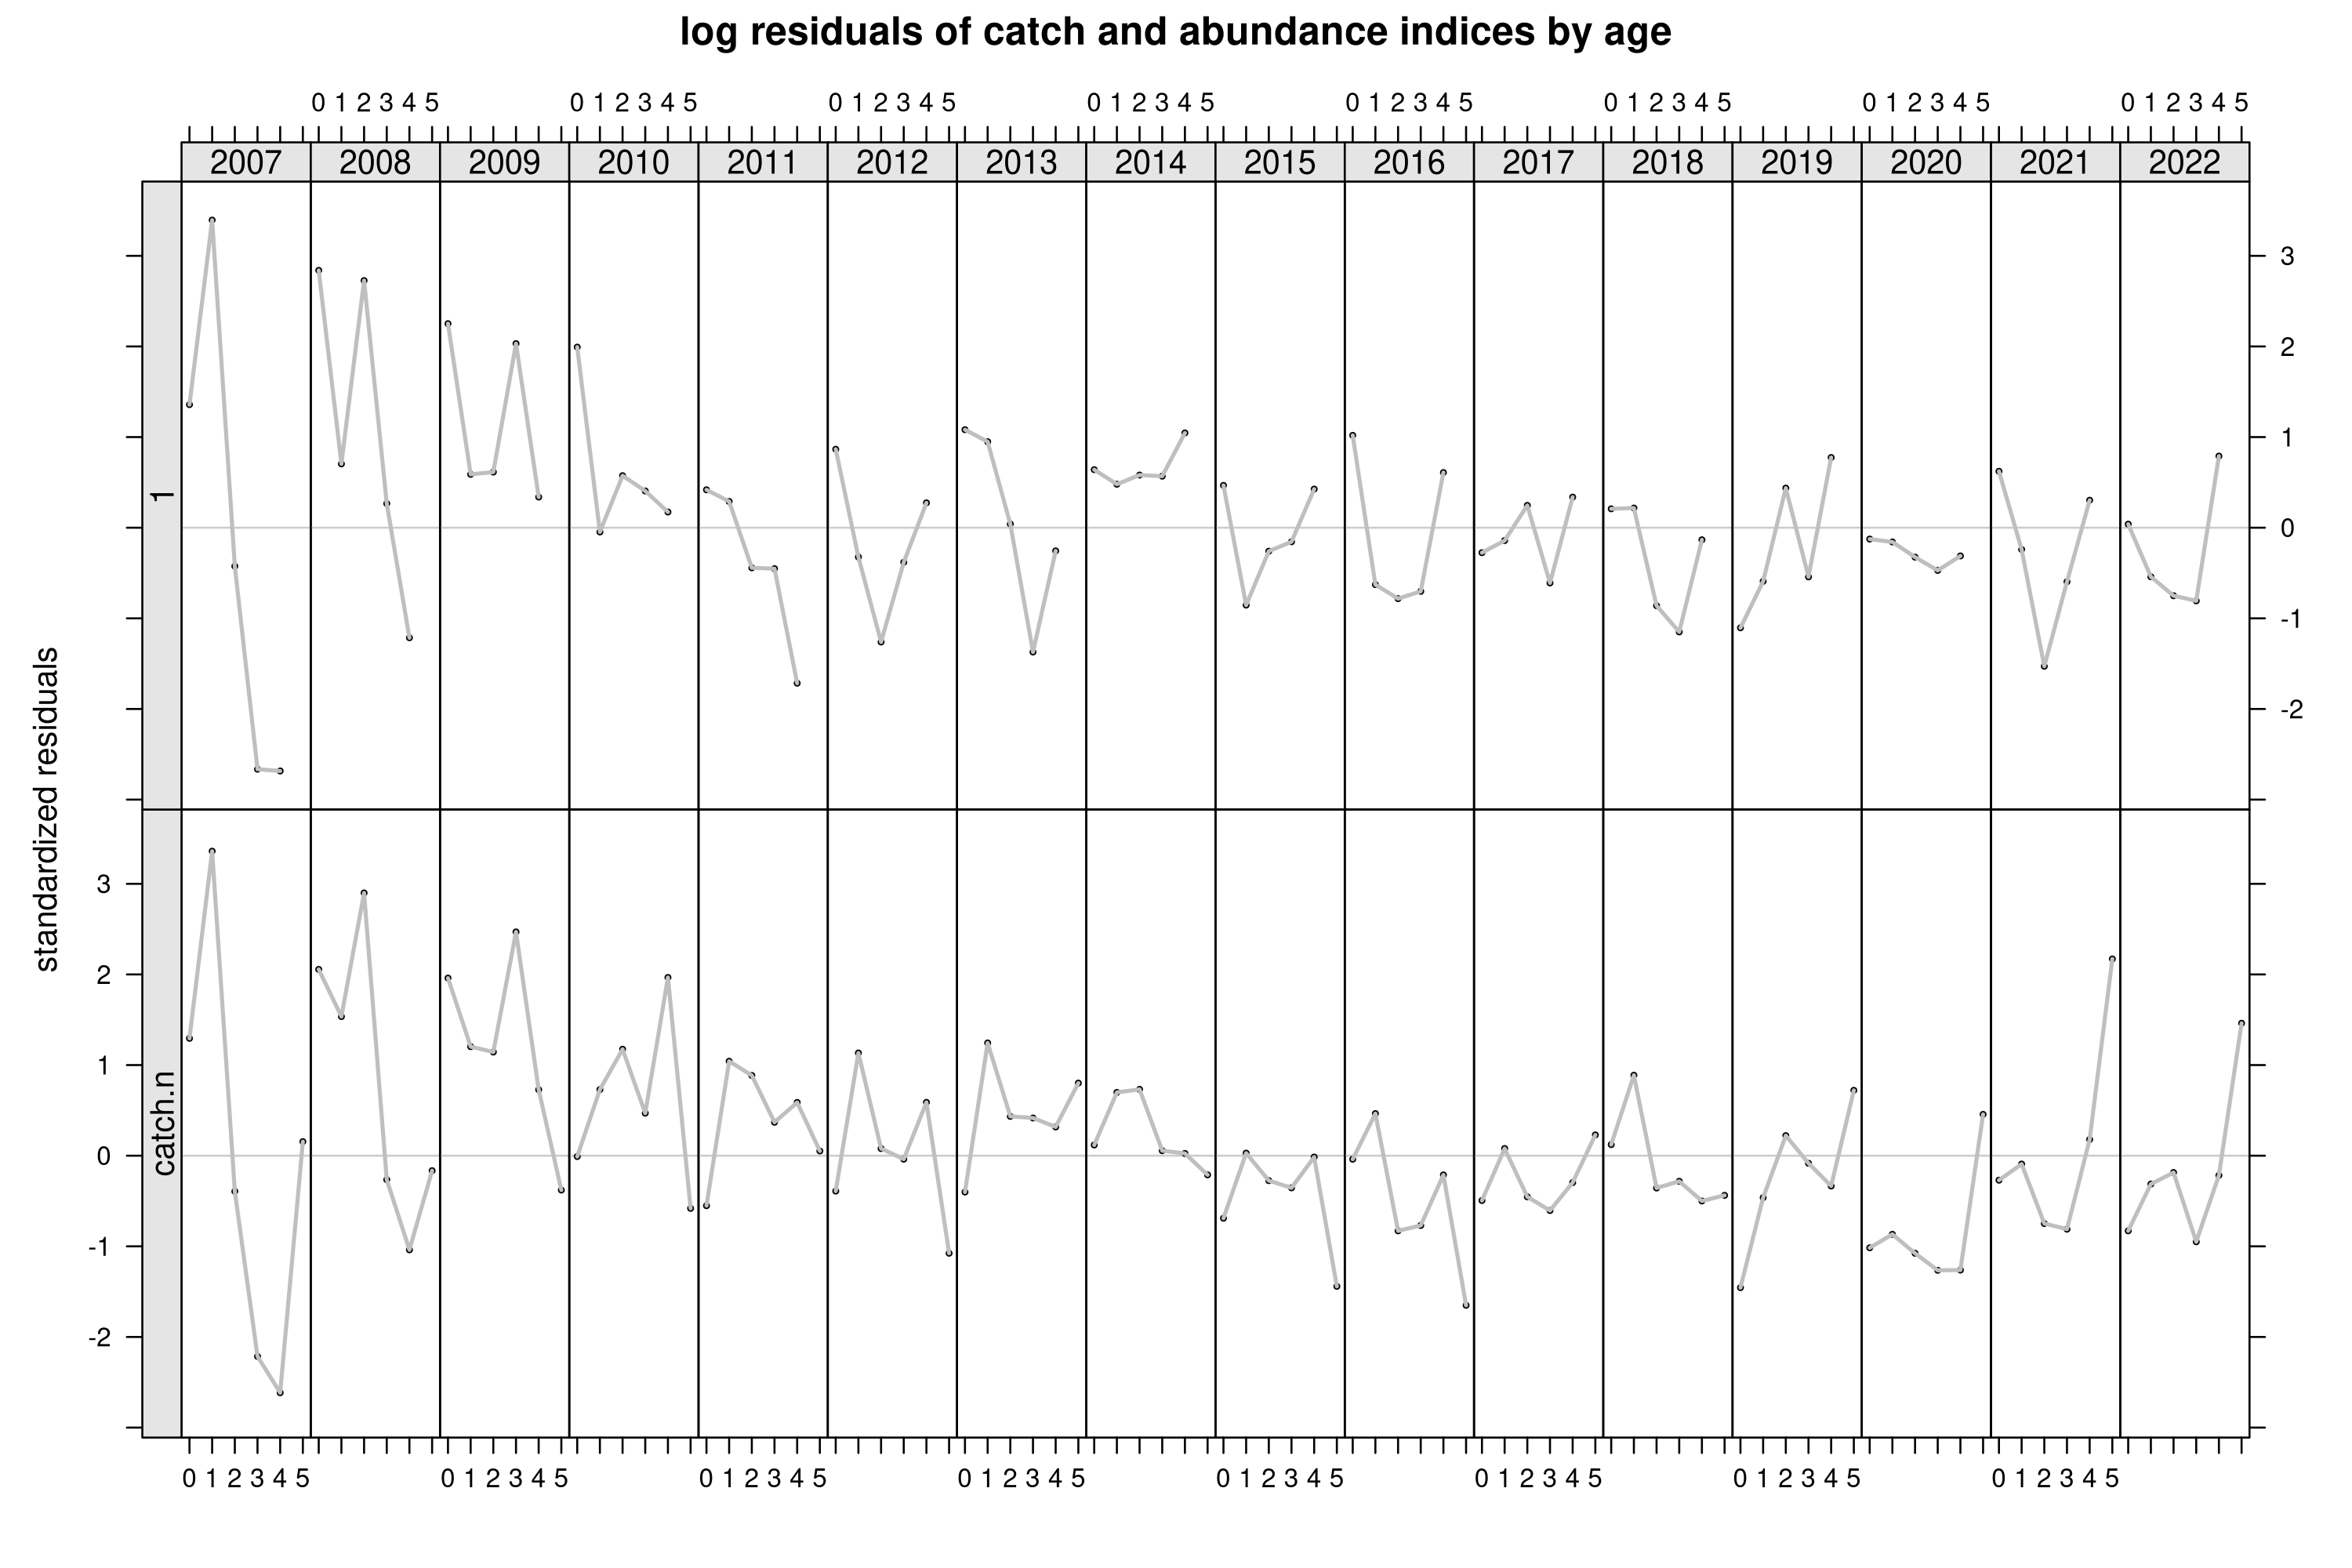
\includegraphics[width=25cm,height=18cm,angle=90]{figure/fageresbyage-1} 

}

\caption[f age effect fit residuals by age)]{f age effect fit residuals by age)}\label{fig:fageresbyage}
\end{figure}

\end{knitrout}

Follwed by the same addition to the catchability model.

\begin{knitrout}
\definecolor{shadecolor}{rgb}{0.949, 0.949, 0.949}\color{fgcolor}\begin{kframe}
\begin{alltt}
\hldef{fit03} \hlkwb{<-} \hlkwd{sca}\hldef{(hke1567, hke1567.idx,} \hlkwc{fmod} \hldef{=} \hlopt{~}\hlnum{1}\hldef{,} \hlkwc{qmod} \hldef{=} \hlkwd{list}\hldef{(}\hlopt{~}\hlkwd{factor}\hldef{(age)),} \hlkwc{srmod} \hldef{=} \hlopt{~}\hlnum{1}\hldef{,}
    \hlkwc{vmod} \hldef{=} \hlkwd{list}\hldef{(}\hlopt{~}\hlnum{1}\hldef{,} \hlopt{~}\hlnum{1}\hldef{),} \hlkwc{n1mod} \hldef{=} \hlopt{~}\hlnum{1}\hldef{)}
\hldef{res03} \hlkwb{<-} \hlkwd{residuals}\hldef{(fit03, hke1567, hke1567.idx)}
\end{alltt}
\end{kframe}
\end{knitrout}

\begin{knitrout}
\definecolor{shadecolor}{rgb}{0.949, 0.949, 0.949}\color{fgcolor}\begin{kframe}
\begin{alltt}
\hlkwd{plot}\hldef{(res03)}
\end{alltt}
\end{kframe}\begin{figure}[H]

{\centering 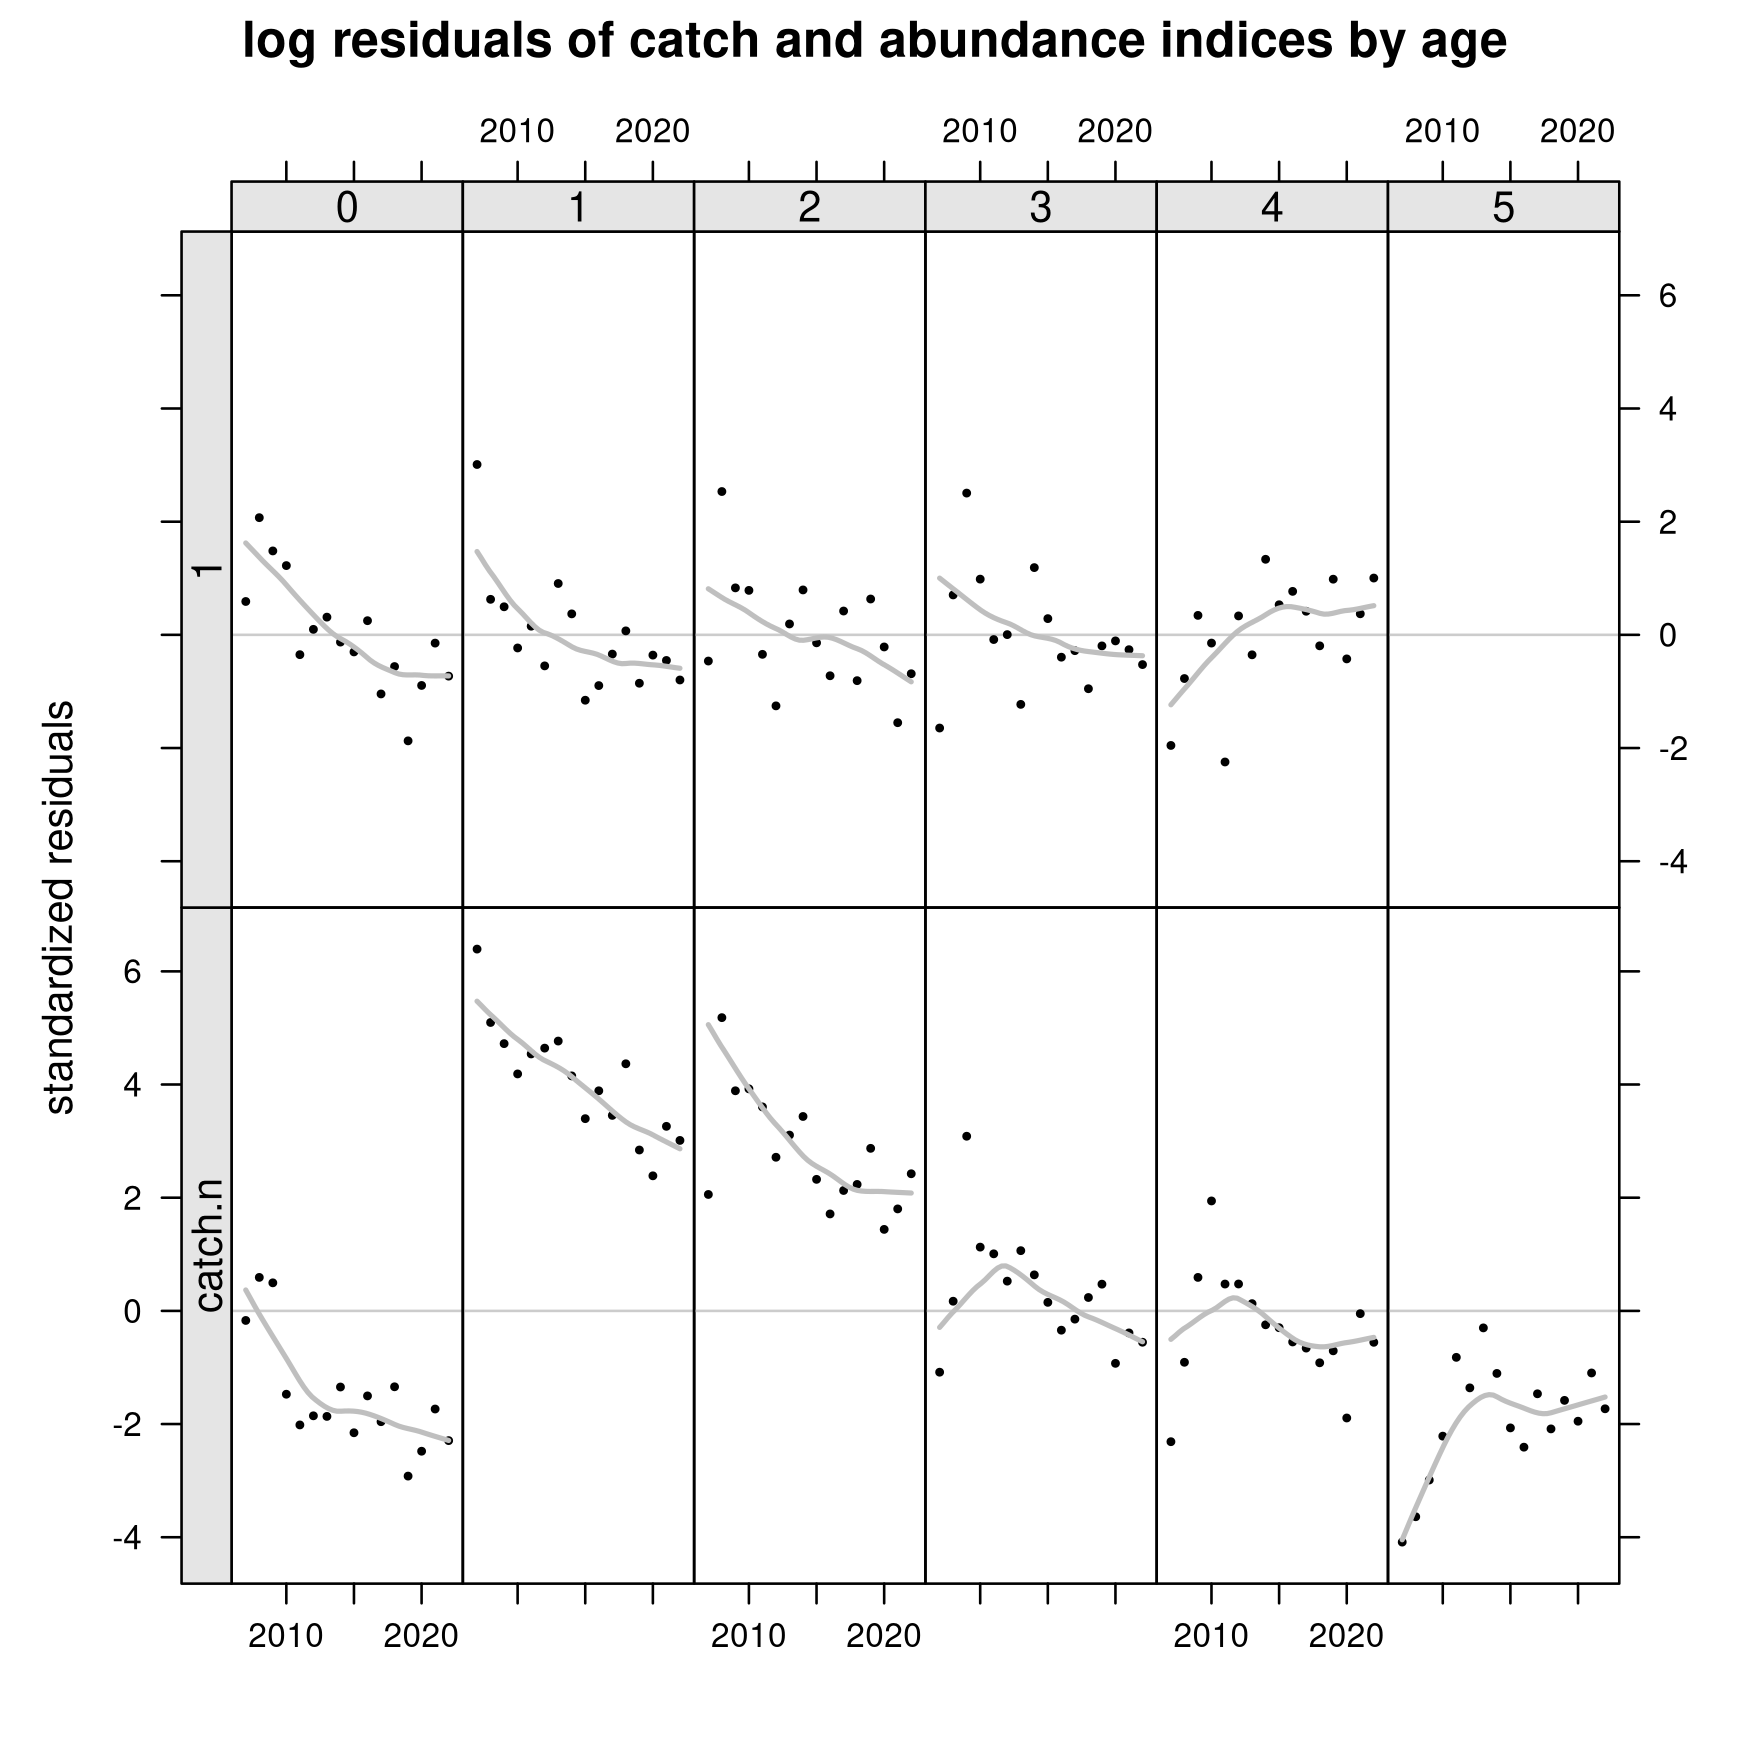
\includegraphics[width=.9\linewidth]{figure/qageresbyyear-1} 

}

\caption[q age effect fit residuals by year)]{q age effect fit residuals by year)}\label{fig:qageresbyyear}
\end{figure}

\end{knitrout}

The residuals plot by age shows the same outcome.  

\begin{knitrout}
\definecolor{shadecolor}{rgb}{0.949, 0.949, 0.949}\color{fgcolor}\begin{kframe}
\begin{alltt}
\hlkwd{plot}\hldef{(res03,} \hlkwc{auxline} \hldef{=} \hlsng{"l"}\hldef{,} \hlkwc{by} \hldef{=} \hlsng{"age"}\hldef{)}
\end{alltt}
\end{kframe}\begin{figure}[H]

{\centering 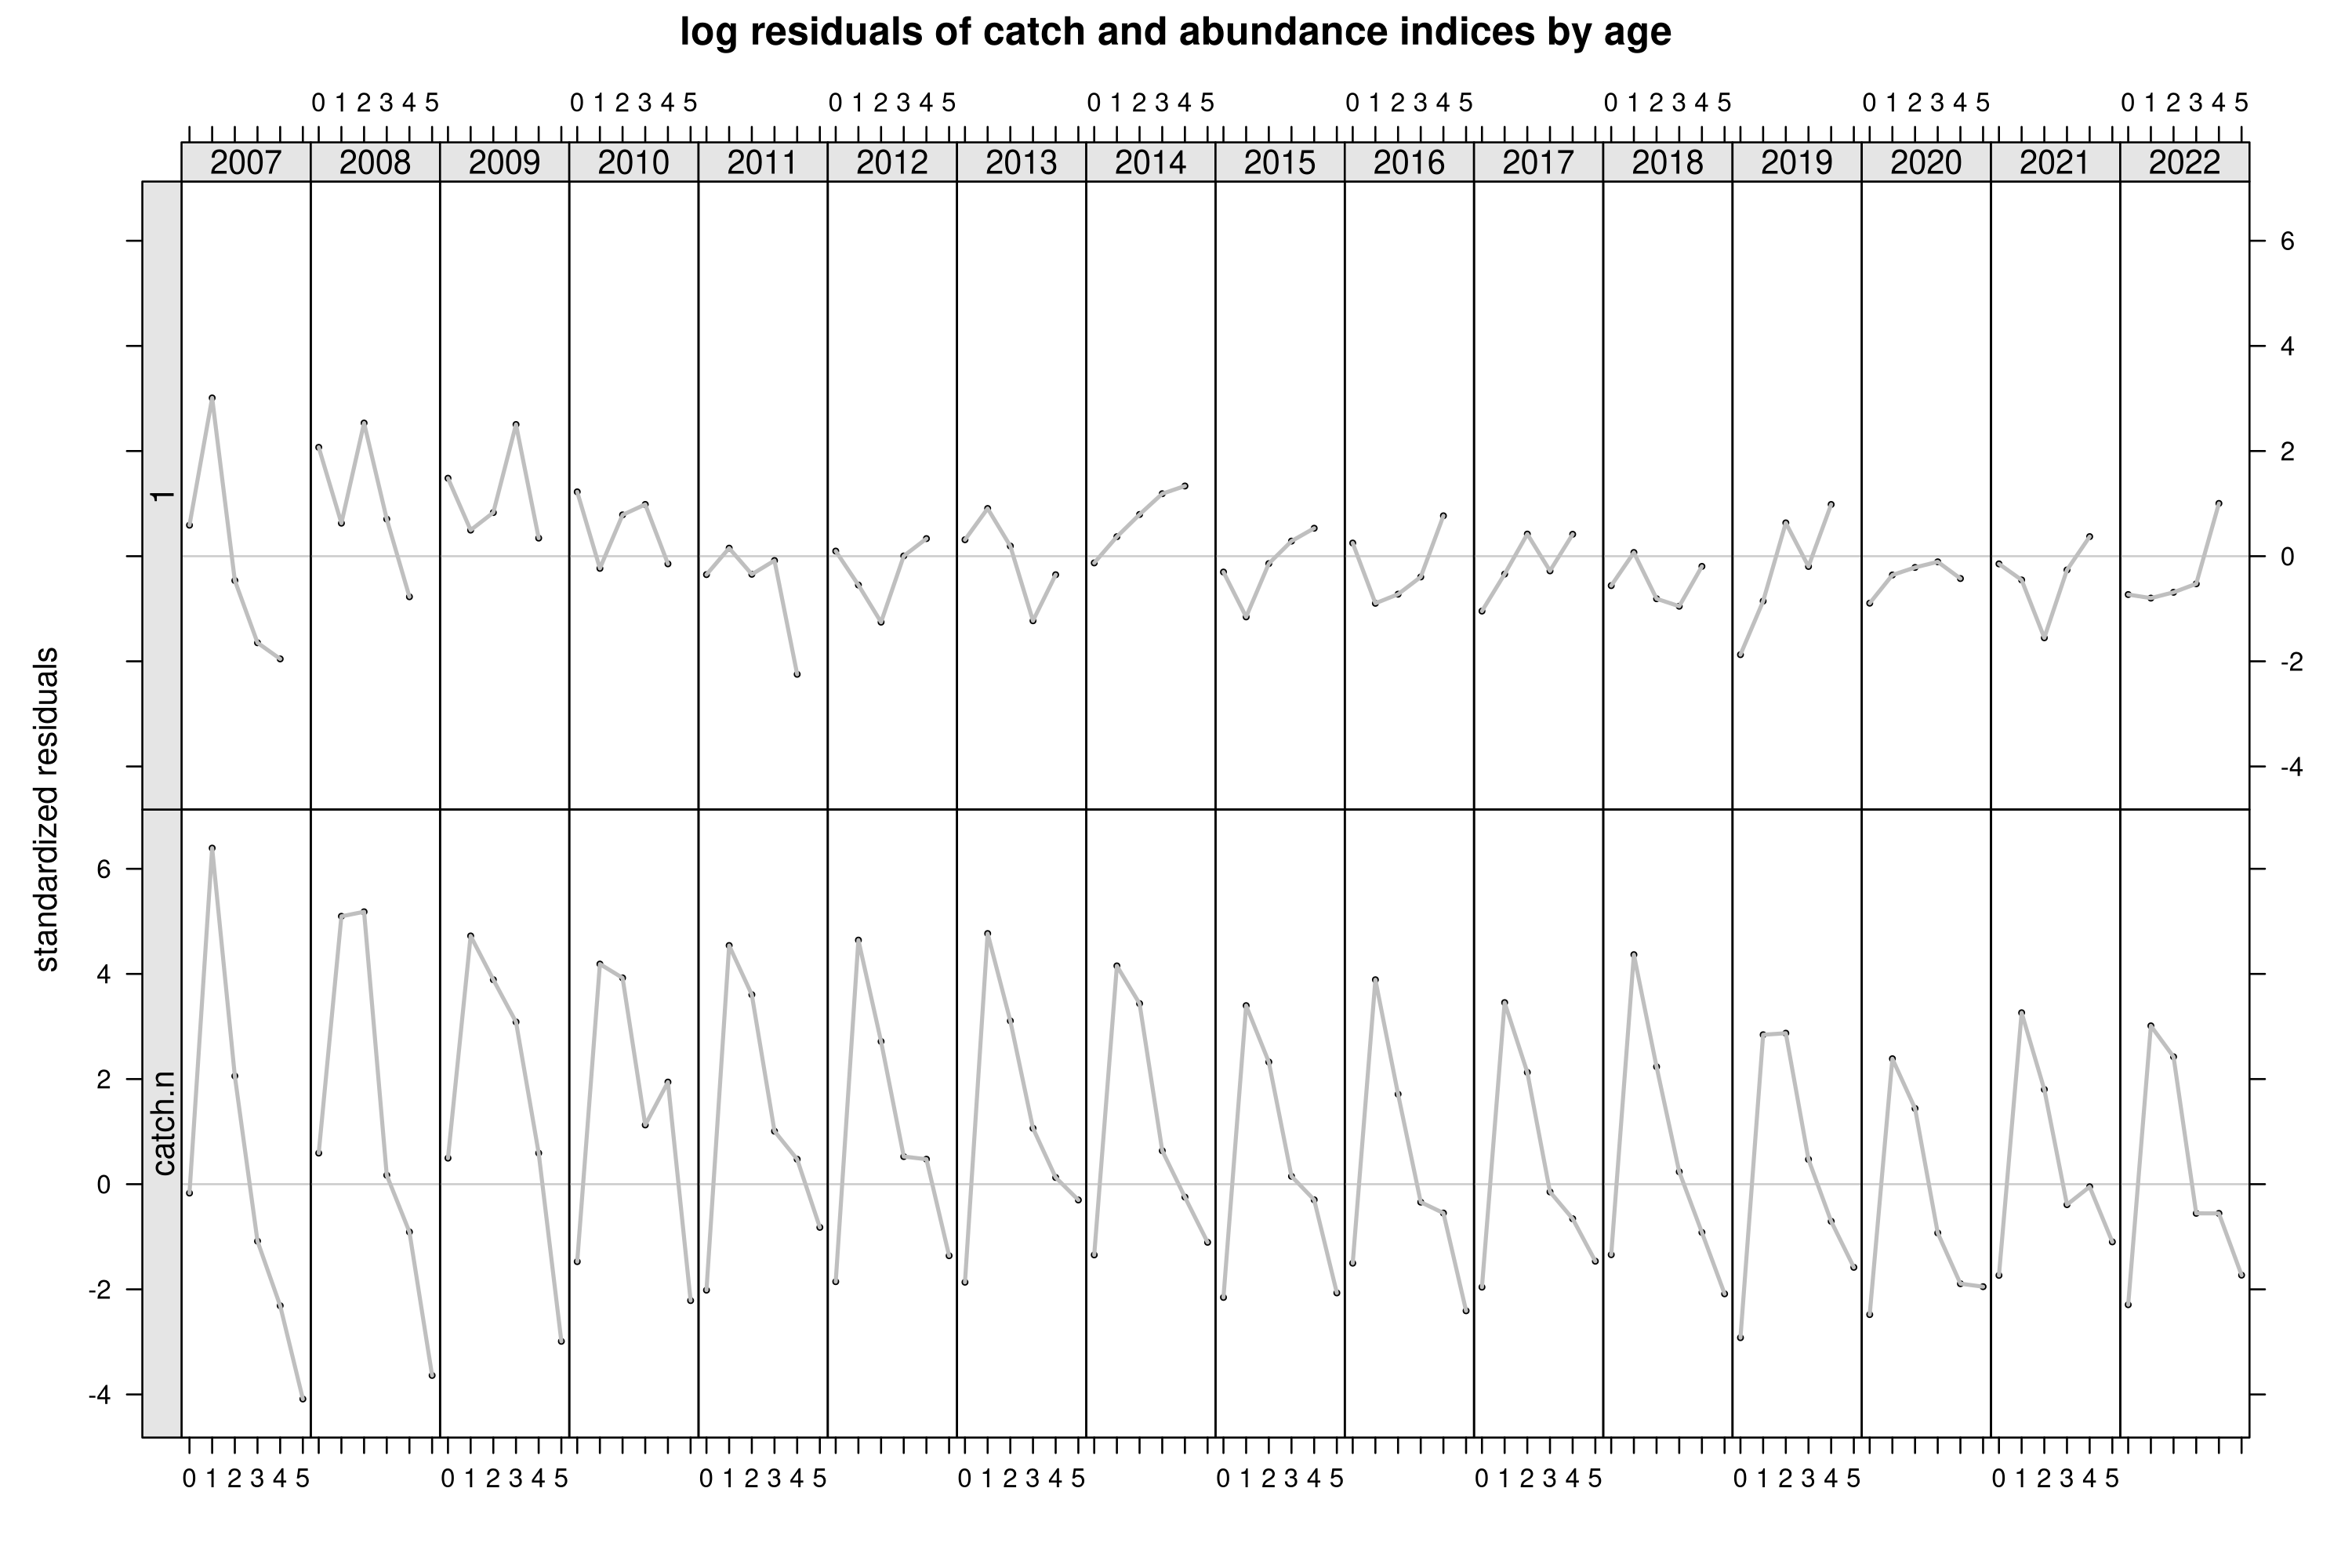
\includegraphics[width=25cm,height=18cm,angle=90]{figure/qageresbyage-1} 

}

\caption[q age effect fit residuals by age)]{q age effect fit residuals by age)}\label{fig:qageresbyage}
\end{figure}

\end{knitrout}

Finally both effects are brought together.

\begin{knitrout}
\definecolor{shadecolor}{rgb}{0.949, 0.949, 0.949}\color{fgcolor}\begin{kframe}
\begin{alltt}
\hldef{fit04} \hlkwb{<-} \hlkwd{sca}\hldef{(hke1567, hke1567.idx,} \hlkwc{fmod} \hldef{=} \hlopt{~}\hlkwd{factor}\hldef{(age),} \hlkwc{qmod} \hldef{=} \hlkwd{list}\hldef{(}\hlopt{~}\hlkwd{factor}\hldef{(age)),}
    \hlkwc{srmod} \hldef{=} \hlopt{~}\hlnum{1}\hldef{,} \hlkwc{vmod} \hldef{=} \hlkwd{list}\hldef{(}\hlopt{~}\hlnum{1}\hldef{,} \hlopt{~}\hlnum{1}\hldef{),} \hlkwc{n1mod} \hldef{=} \hlopt{~}\hlnum{1}\hldef{)}
\hldef{res04} \hlkwb{<-} \hlkwd{residuals}\hldef{(fit04, hke1567, hke1567.idx)}
\end{alltt}
\end{kframe}
\end{knitrout}

\begin{knitrout}
\definecolor{shadecolor}{rgb}{0.949, 0.949, 0.949}\color{fgcolor}\begin{kframe}
\begin{alltt}
\hlkwd{plot}\hldef{(res04)}
\end{alltt}
\end{kframe}\begin{figure}[H]

{\centering 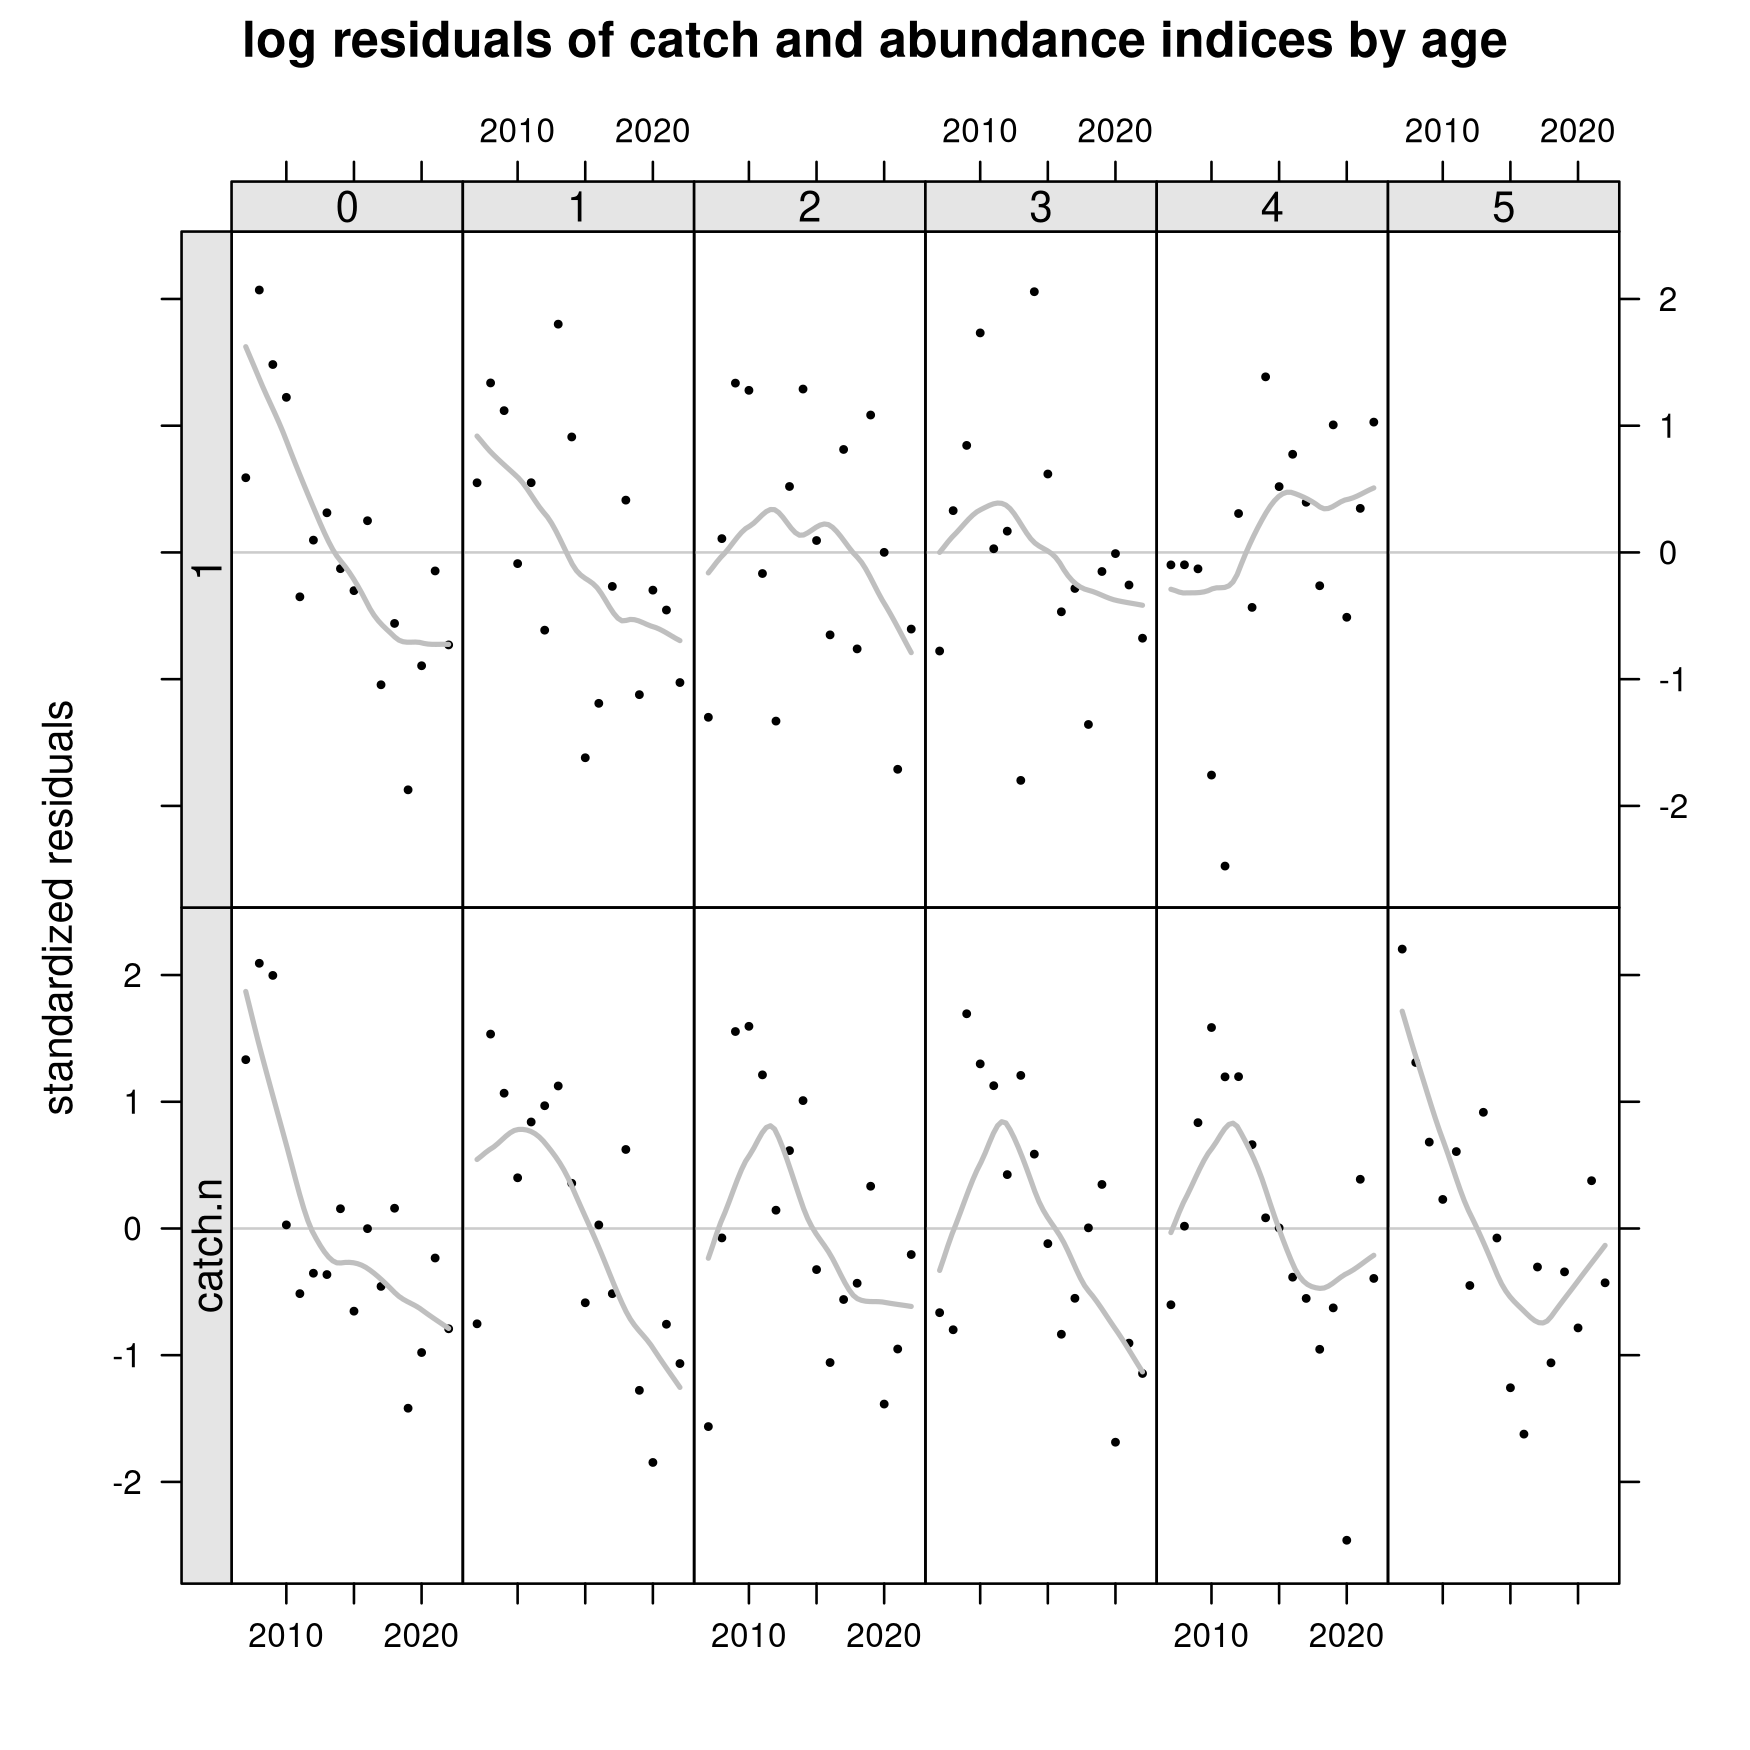
\includegraphics[width=.9\linewidth]{figure/fqageresbyyear-1} 

}

\caption[q age effect fit residuals by year)]{q age effect fit residuals by year)}\label{fig:fqageresbyyear}
\end{figure}

\end{knitrout}

The residuals plot by age shows the same outcome.  

\begin{knitrout}
\definecolor{shadecolor}{rgb}{0.949, 0.949, 0.949}\color{fgcolor}\begin{kframe}
\begin{alltt}
\hlkwd{plot}\hldef{(res04,} \hlkwc{auxline} \hldef{=} \hlsng{"l"}\hldef{,} \hlkwc{by} \hldef{=} \hlsng{"age"}\hldef{)}
\end{alltt}
\end{kframe}\begin{figure}[H]

{\centering 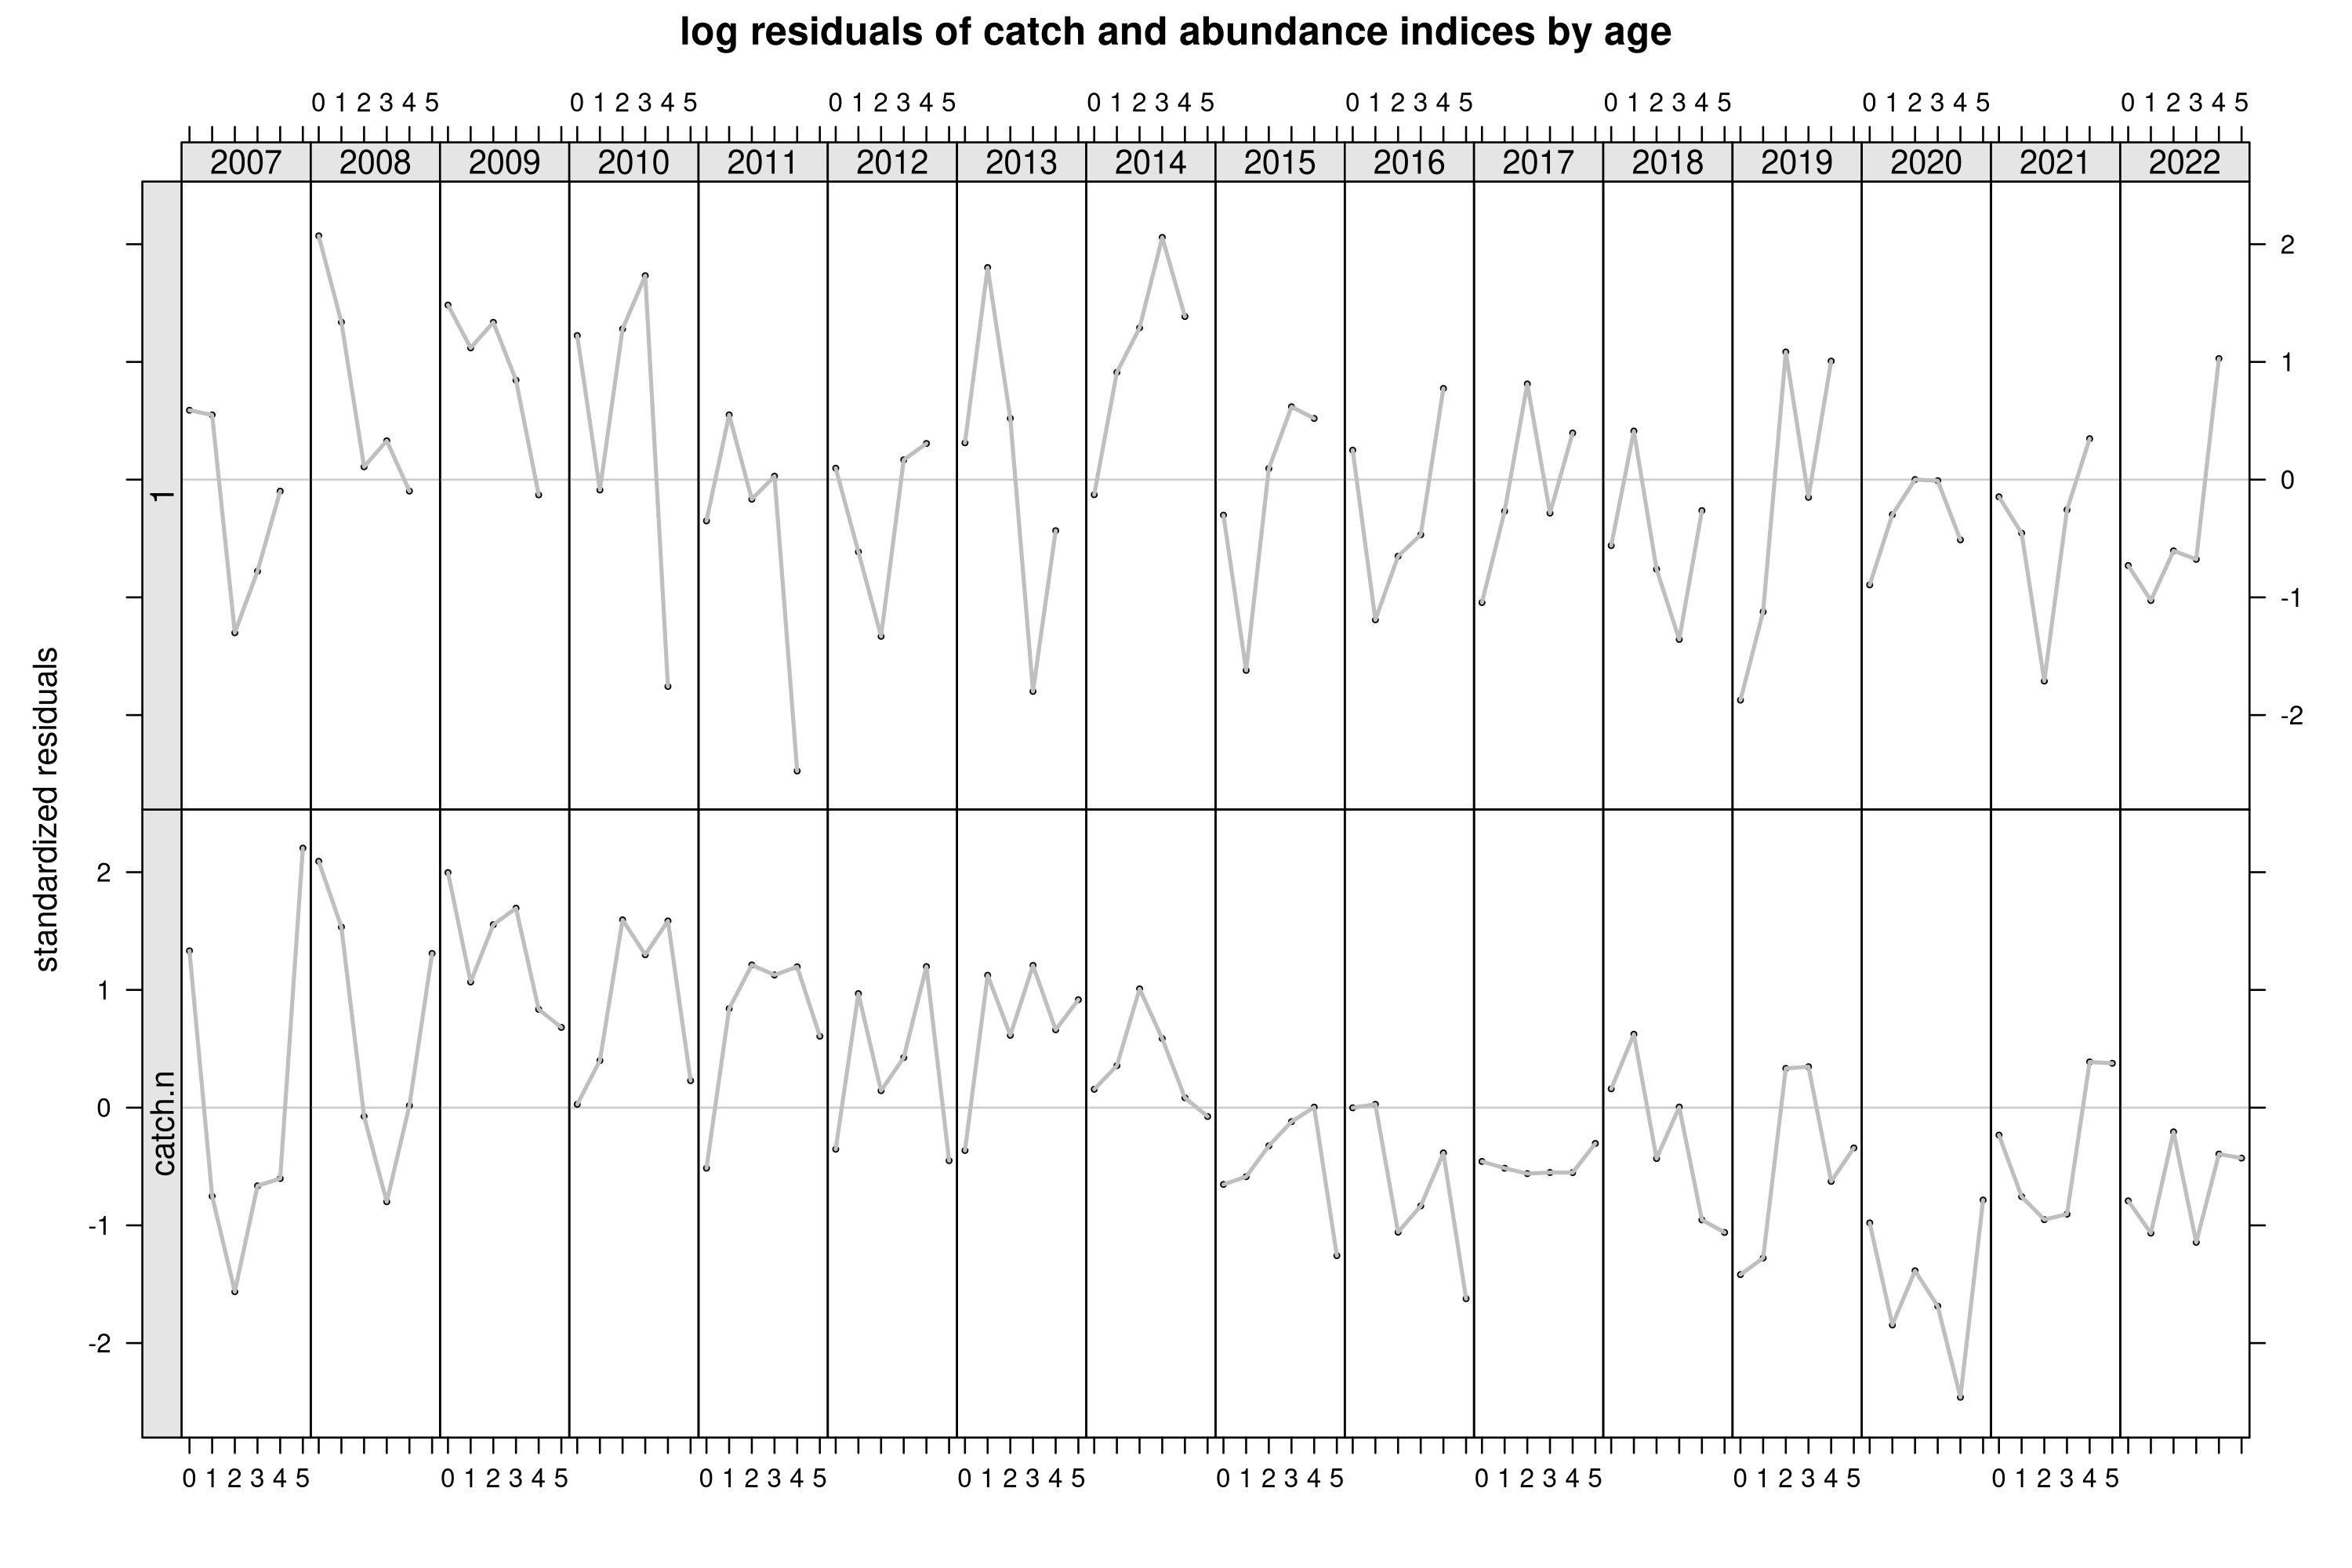
\includegraphics[width=25cm,height=18cm,angle=90]{figure/fqageresbyage-1} 

}

\caption[q age effect fit residuals by age)]{q age effect fit residuals by age)}\label{fig:fqageresbyage}
\end{figure}

\end{knitrout}

\subsection{The fishing mortality year model}

This model will introduce an year effect in the fishing mortality submodel on top of the age effects added before.

\begin{knitrout}
\definecolor{shadecolor}{rgb}{0.949, 0.949, 0.949}\color{fgcolor}\begin{kframe}
\begin{alltt}
\hldef{fit05} \hlkwb{<-} \hlkwd{sca}\hldef{(hke1567, hke1567.idx,} \hlkwc{fmod} \hldef{=} \hlopt{~}\hlkwd{factor}\hldef{(age)} \hlopt{+} \hlkwd{factor}\hldef{(year),} \hlkwc{qmod} \hldef{=} \hlkwd{list}\hldef{(}\hlopt{~}\hlkwd{factor}\hldef{(age)),}
    \hlkwc{srmod} \hldef{=} \hlopt{~}\hlnum{1}\hldef{,} \hlkwc{vmod} \hldef{=} \hlkwd{list}\hldef{(}\hlopt{~}\hlnum{1}\hldef{,} \hlopt{~}\hlnum{1}\hldef{),} \hlkwc{n1mod} \hldef{=} \hlopt{~}\hlnum{1}\hldef{)}
\hldef{res05} \hlkwb{<-} \hlkwd{residuals}\hldef{(fit05, hke1567, hke1567.idx)}
\end{alltt}
\end{kframe}
\end{knitrout}

The residuals plot now shows catch at age residuals stagered as before. The year trends are less pronounced although, because the data doesn't have a very strong year effect, it's less clear than when modelling the age effect. 

\begin{knitrout}
\definecolor{shadecolor}{rgb}{0.949, 0.949, 0.949}\color{fgcolor}\begin{kframe}
\begin{alltt}
\hlkwd{plot}\hldef{(res05)}
\end{alltt}
\end{kframe}\begin{figure}[H]

{\centering 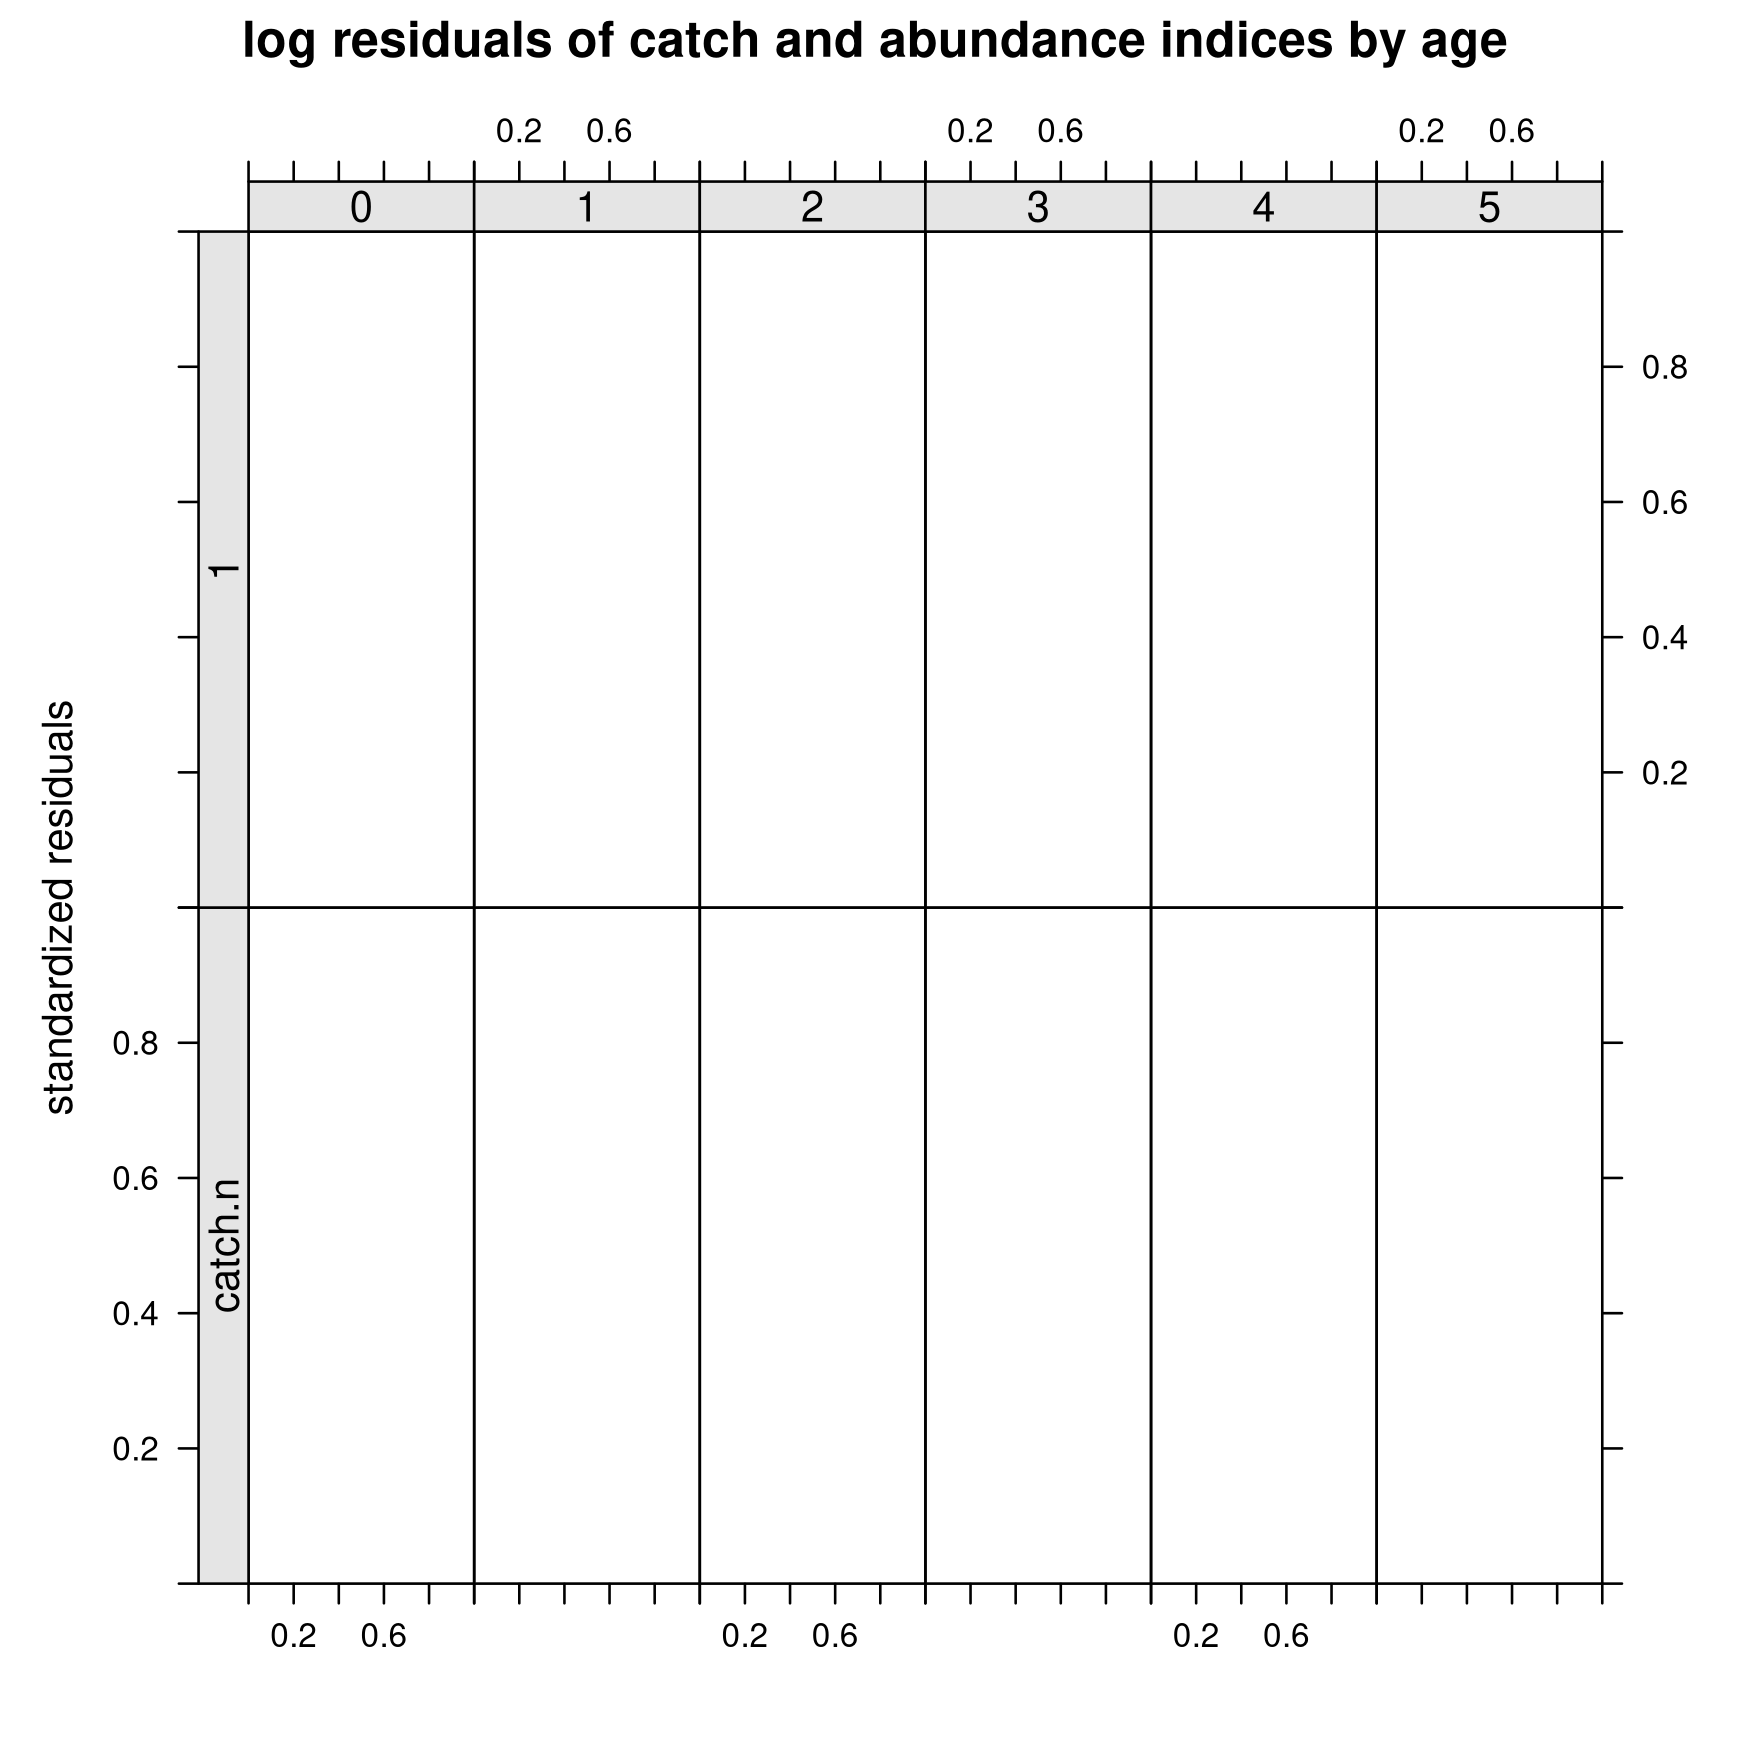
\includegraphics[width=.9\linewidth]{figure/fyearresbyyear-1} 

}

\caption[f year effect fit residuals by year)]{f year effect fit residuals by year)}\label{fig:fyearresbyyear}
\end{figure}

\end{knitrout}

The residuals plot by age shows the same outcome.  

\begin{knitrout}
\definecolor{shadecolor}{rgb}{0.949, 0.949, 0.949}\color{fgcolor}\begin{kframe}
\begin{alltt}
\hlkwd{plot}\hldef{(res05,} \hlkwc{auxline} \hldef{=} \hlsng{"l"}\hldef{,} \hlkwc{by} \hldef{=} \hlsng{"age"}\hldef{)}
\end{alltt}
\end{kframe}\begin{figure}[H]

{\centering 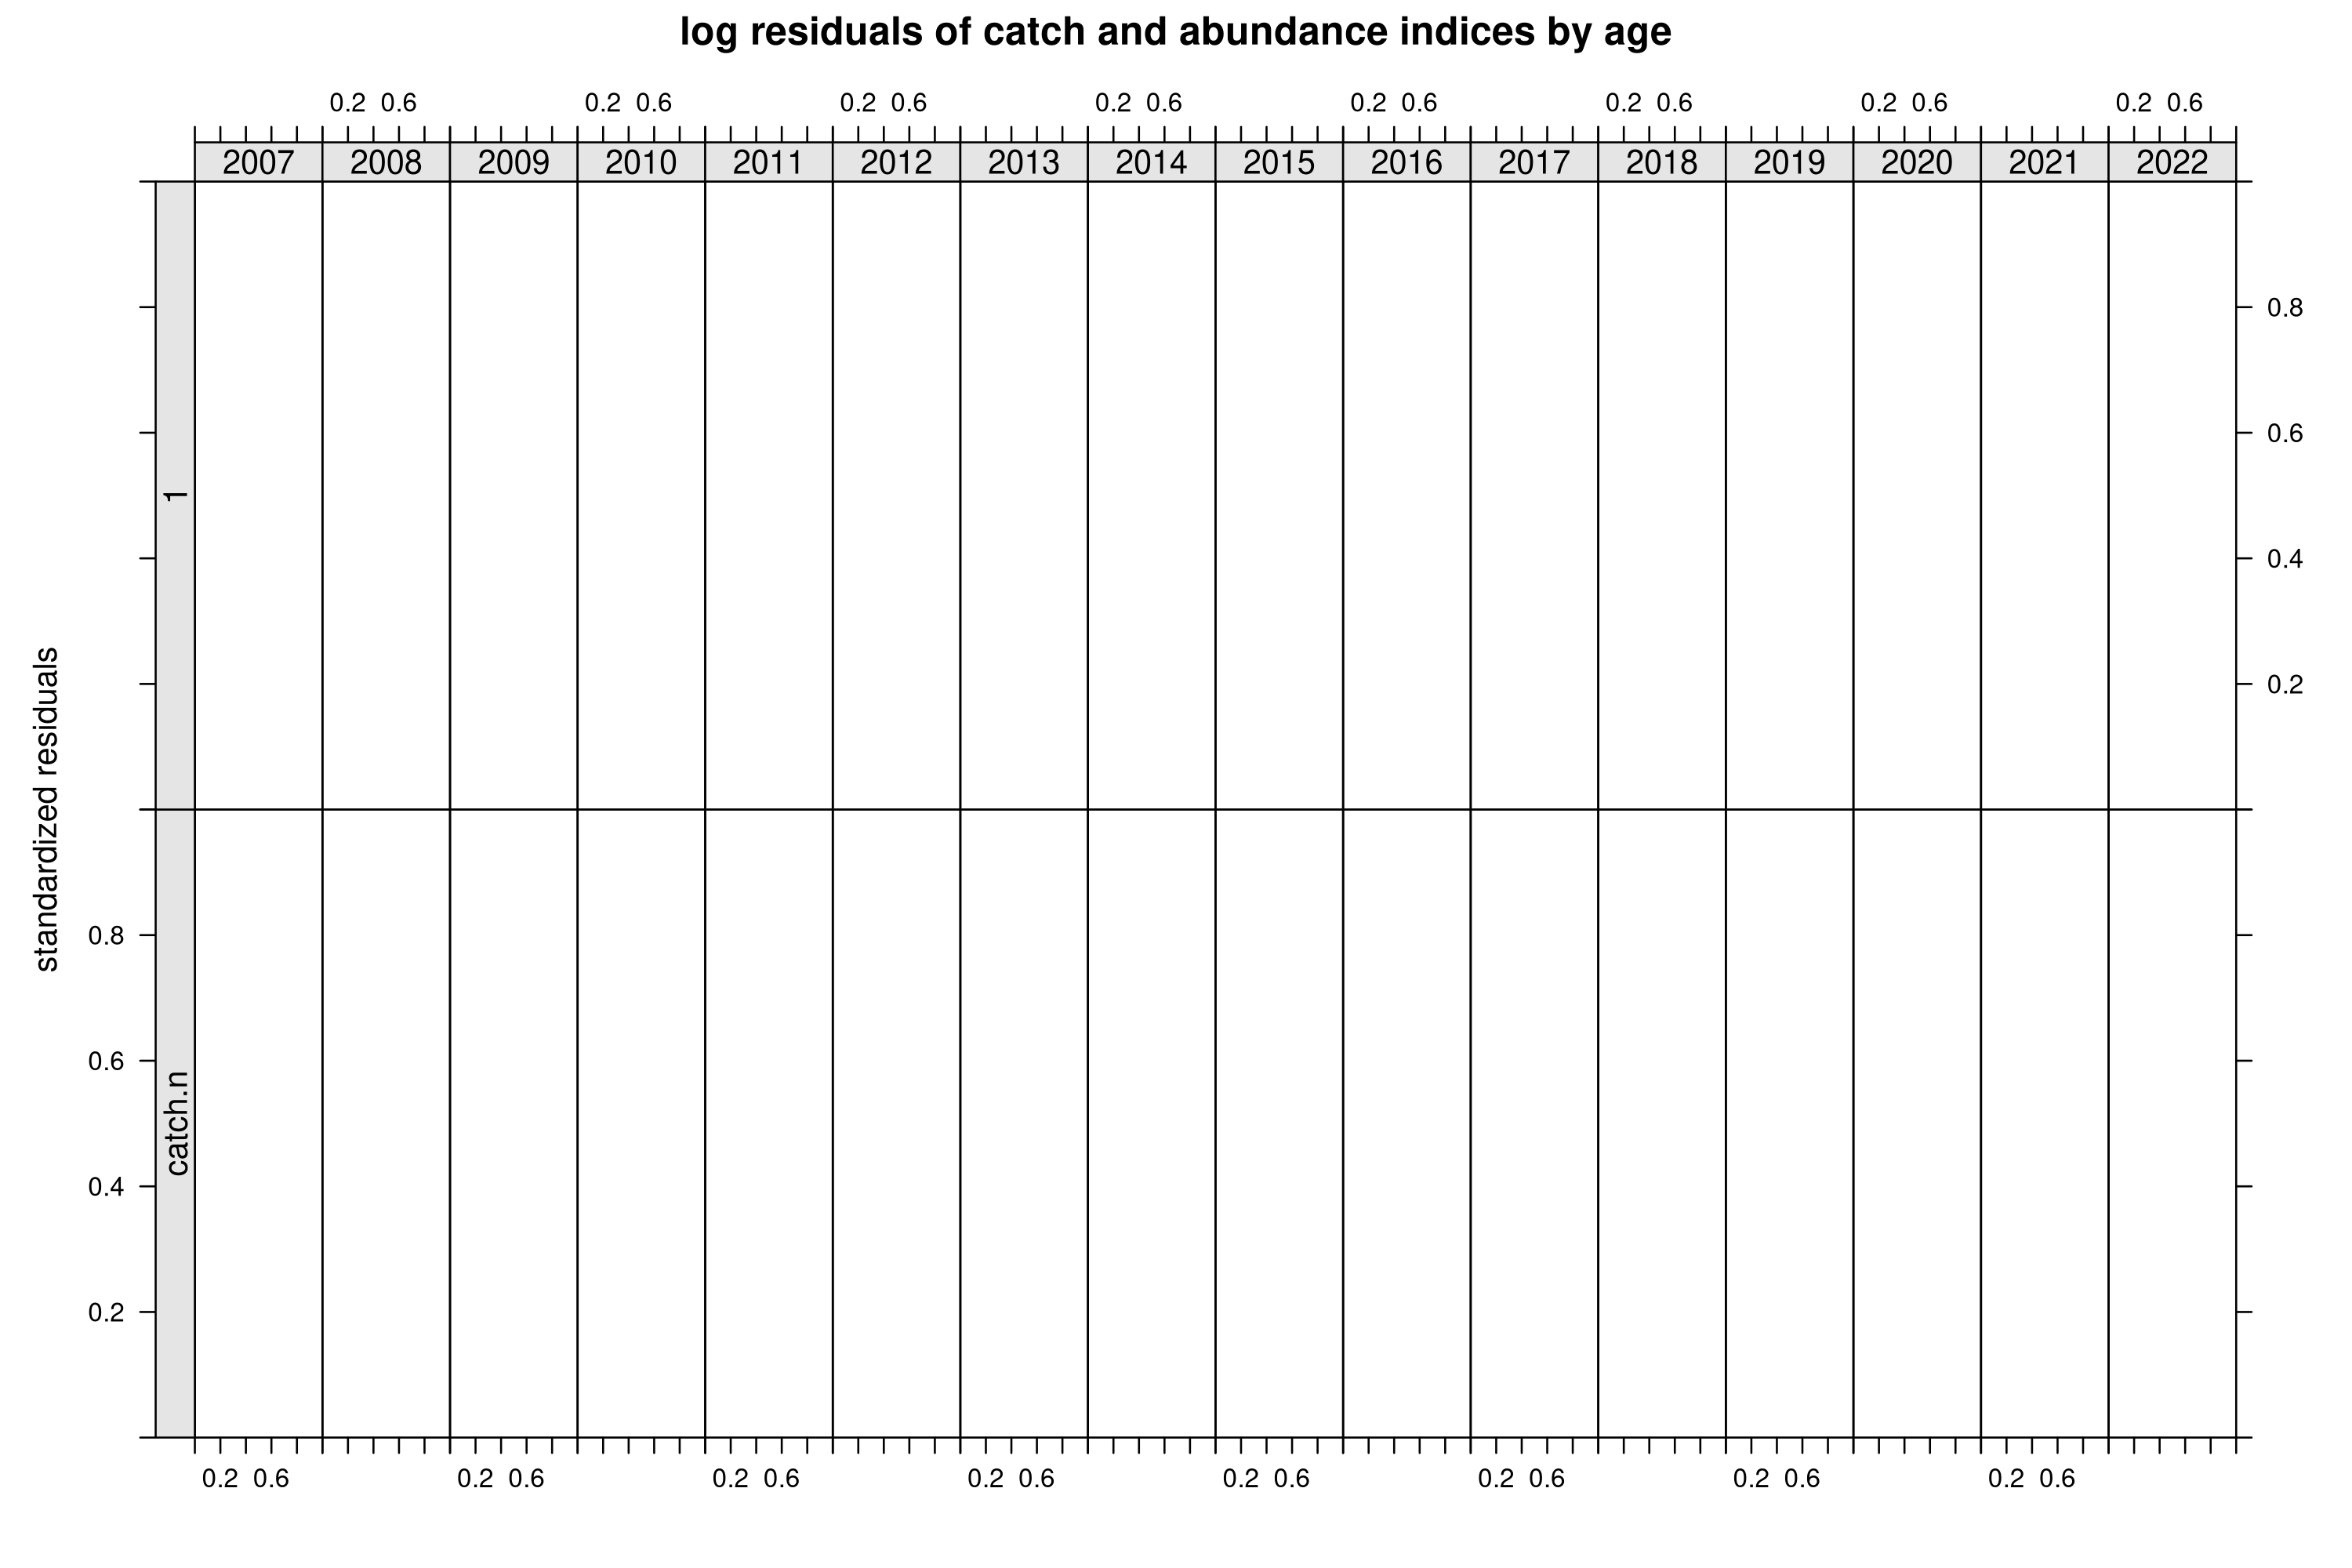
\includegraphics[width=25cm,height=18cm,angle=90]{figure/fyearresbyage-1} 

}

\caption[f year effect fit residuals by age)]{f year effect fit residuals by age)}\label{fig:fyearresbyage}
\end{figure}

\end{knitrout}

We can see now that the residuals show a lot less patterns than before. There's still some issues, the survey catchability seems to have an year trend. However the model is not fully specified yet, stock recruitment is modelled as constant over time, the initial population abundance is also modelled as a constant as well as the variance models.

\subsection{The initial year population abundance model, aka N1 }

This model will introduce an age effect in the population abundance in the first year of the time series. This model sets the n-at-age in the first year of the time series, which is needed due to the lack of previous data to reconstruct those cohorts.

\begin{knitrout}
\definecolor{shadecolor}{rgb}{0.949, 0.949, 0.949}\color{fgcolor}\begin{kframe}
\begin{alltt}
\hldef{fit06} \hlkwb{<-} \hlkwd{sca}\hldef{(hke1567, hke1567.idx,} \hlkwc{fmod} \hldef{=} \hlopt{~}\hlkwd{factor}\hldef{(age)} \hlopt{+} \hlkwd{factor}\hldef{(year),} \hlkwc{qmod} \hldef{=} \hlkwd{list}\hldef{(}\hlopt{~}\hlkwd{factor}\hldef{(age)),}
    \hlkwc{srmod} \hldef{=} \hlopt{~}\hlnum{1}\hldef{,} \hlkwc{vmod} \hldef{=} \hlkwd{list}\hldef{(}\hlopt{~}\hlnum{1}\hldef{,} \hlopt{~}\hlnum{1}\hldef{),} \hlkwc{n1mod} \hldef{=} \hlopt{~}\hlkwd{factor}\hldef{(age))}
\hldef{res06} \hlkwb{<-} \hlkwd{residuals}\hldef{(fit06, hke1567, hke1567.idx)}
\end{alltt}
\end{kframe}
\end{knitrout}

The residuals plot now shows catch at age residuals stagered as before. The year trends are less pronounced although, because the data doesn't have a very strong year effect, it's less clear than when modelling the age effect. 

\begin{knitrout}
\definecolor{shadecolor}{rgb}{0.949, 0.949, 0.949}\color{fgcolor}\begin{kframe}
\begin{alltt}
\hlkwd{plot}\hldef{(res06)}
\end{alltt}
\end{kframe}\begin{figure}[H]

{\centering 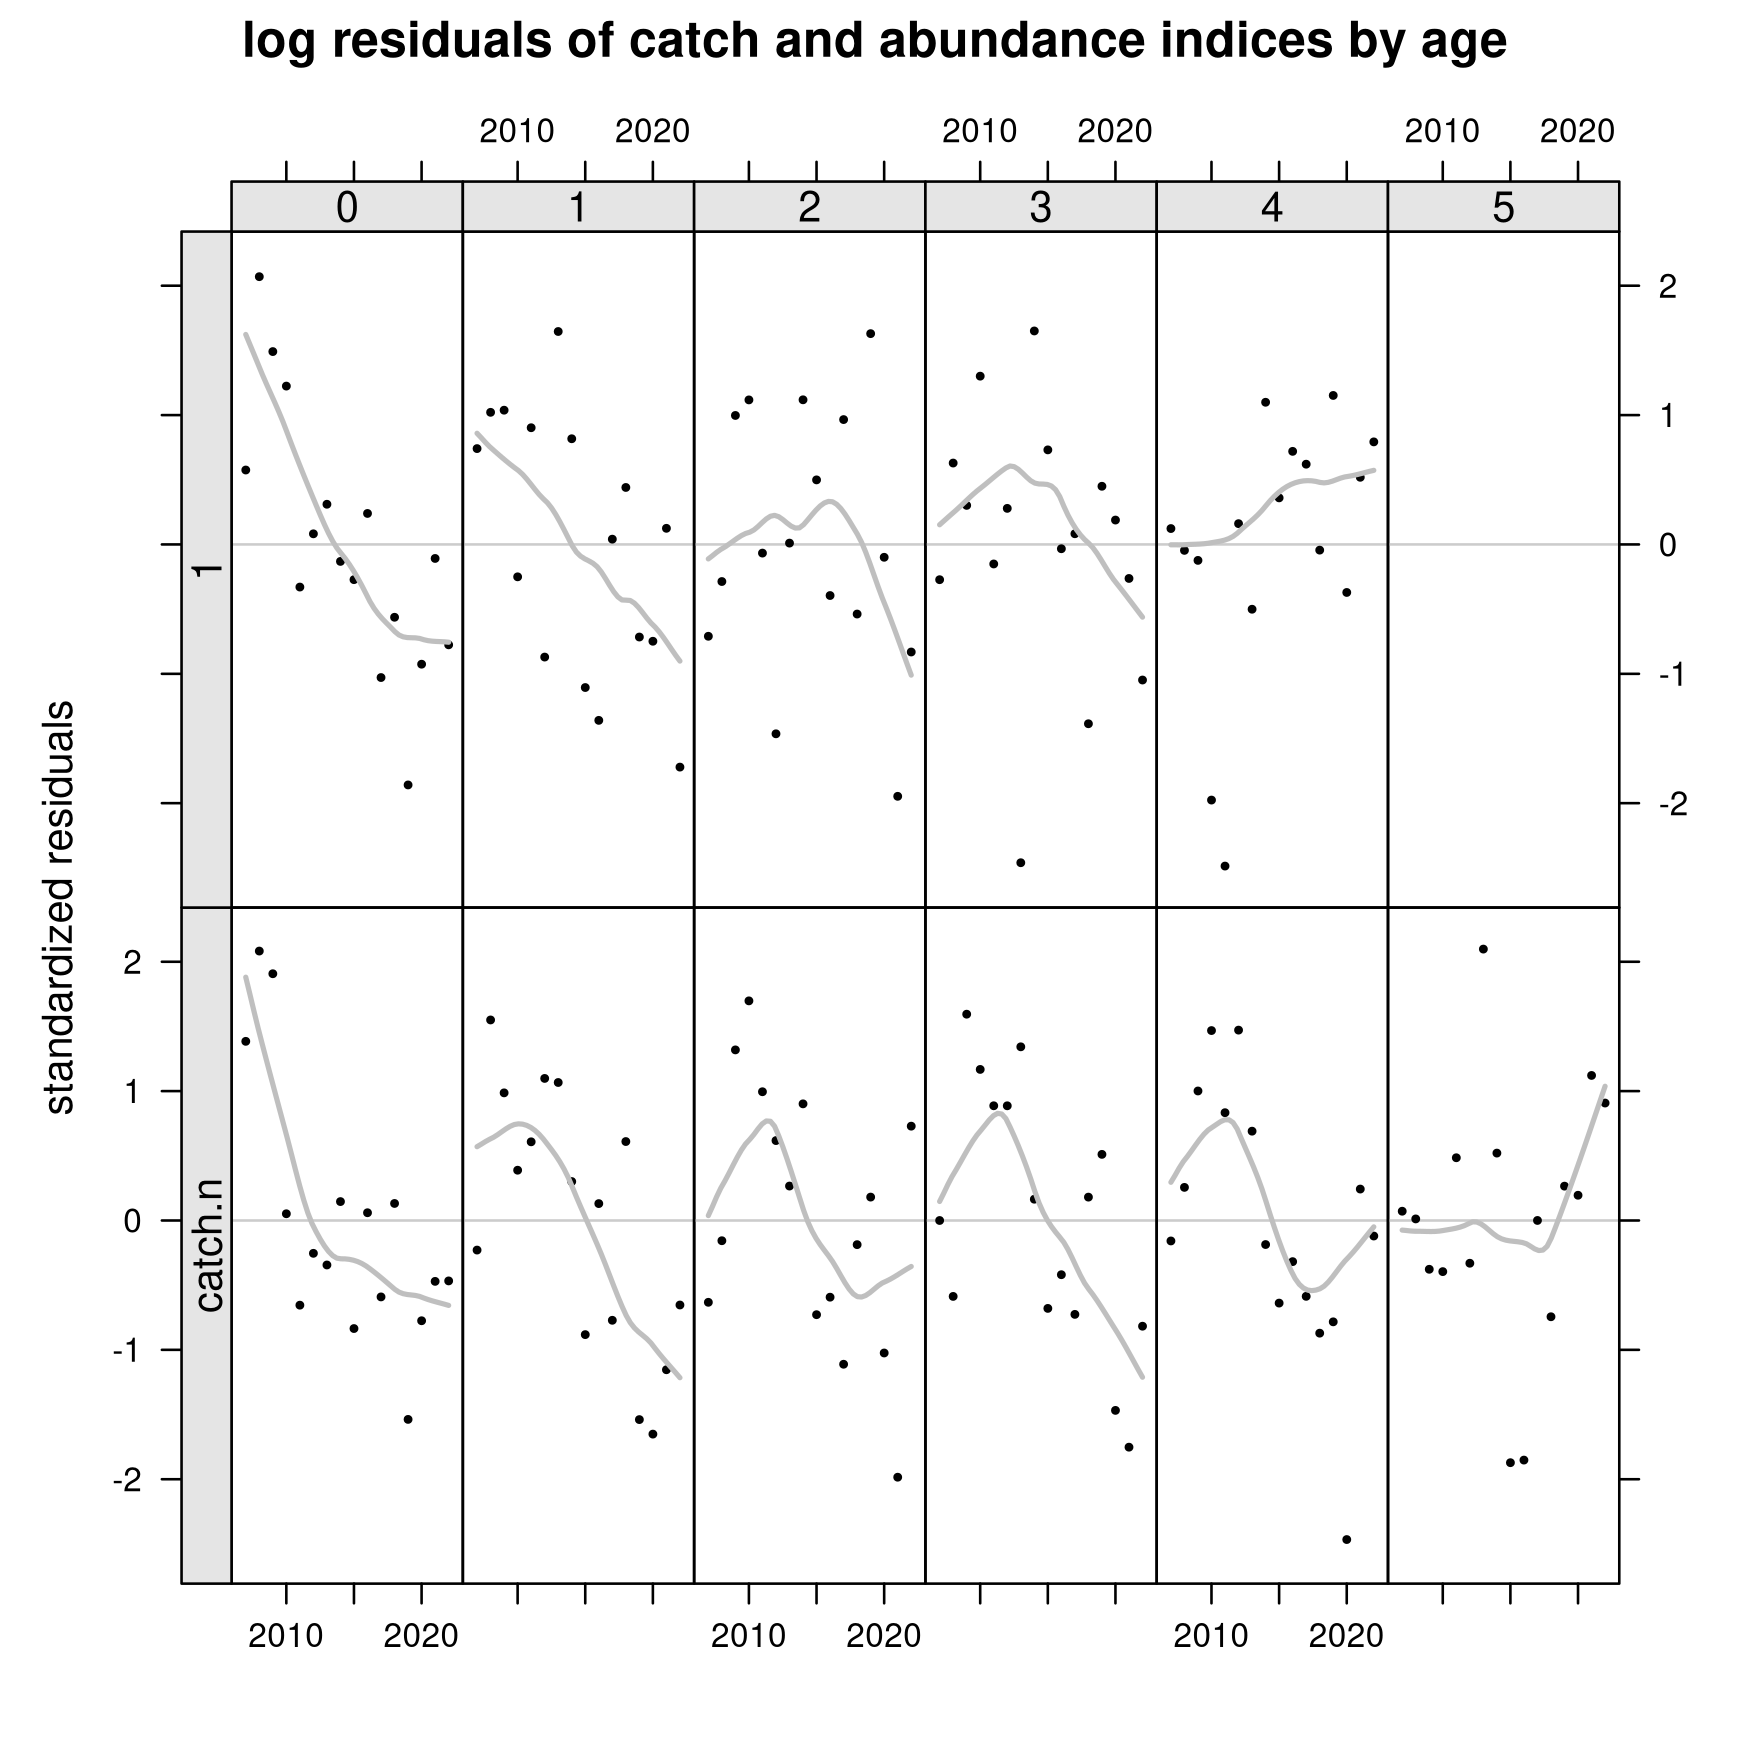
\includegraphics[width=.9\linewidth]{figure/n1arresbyyear-1} 

}

\caption[f year effect fit residuals by year)]{f year effect fit residuals by year)}\label{fig:n1arresbyyear}
\end{figure}

\end{knitrout}

The residuals by age (figure~\ref{fig:n1resbyage}) the residuals' improvement in the first year of the catch at age time series (bottom left plots).  

\begin{knitrout}
\definecolor{shadecolor}{rgb}{0.949, 0.949, 0.949}\color{fgcolor}\begin{kframe}
\begin{alltt}
\hlkwd{plot}\hldef{(res06,} \hlkwc{auxline} \hldef{=} \hlsng{"l"}\hldef{,} \hlkwc{by} \hldef{=} \hlsng{"age"}\hldef{)}
\end{alltt}
\end{kframe}\begin{figure}[H]

{\centering 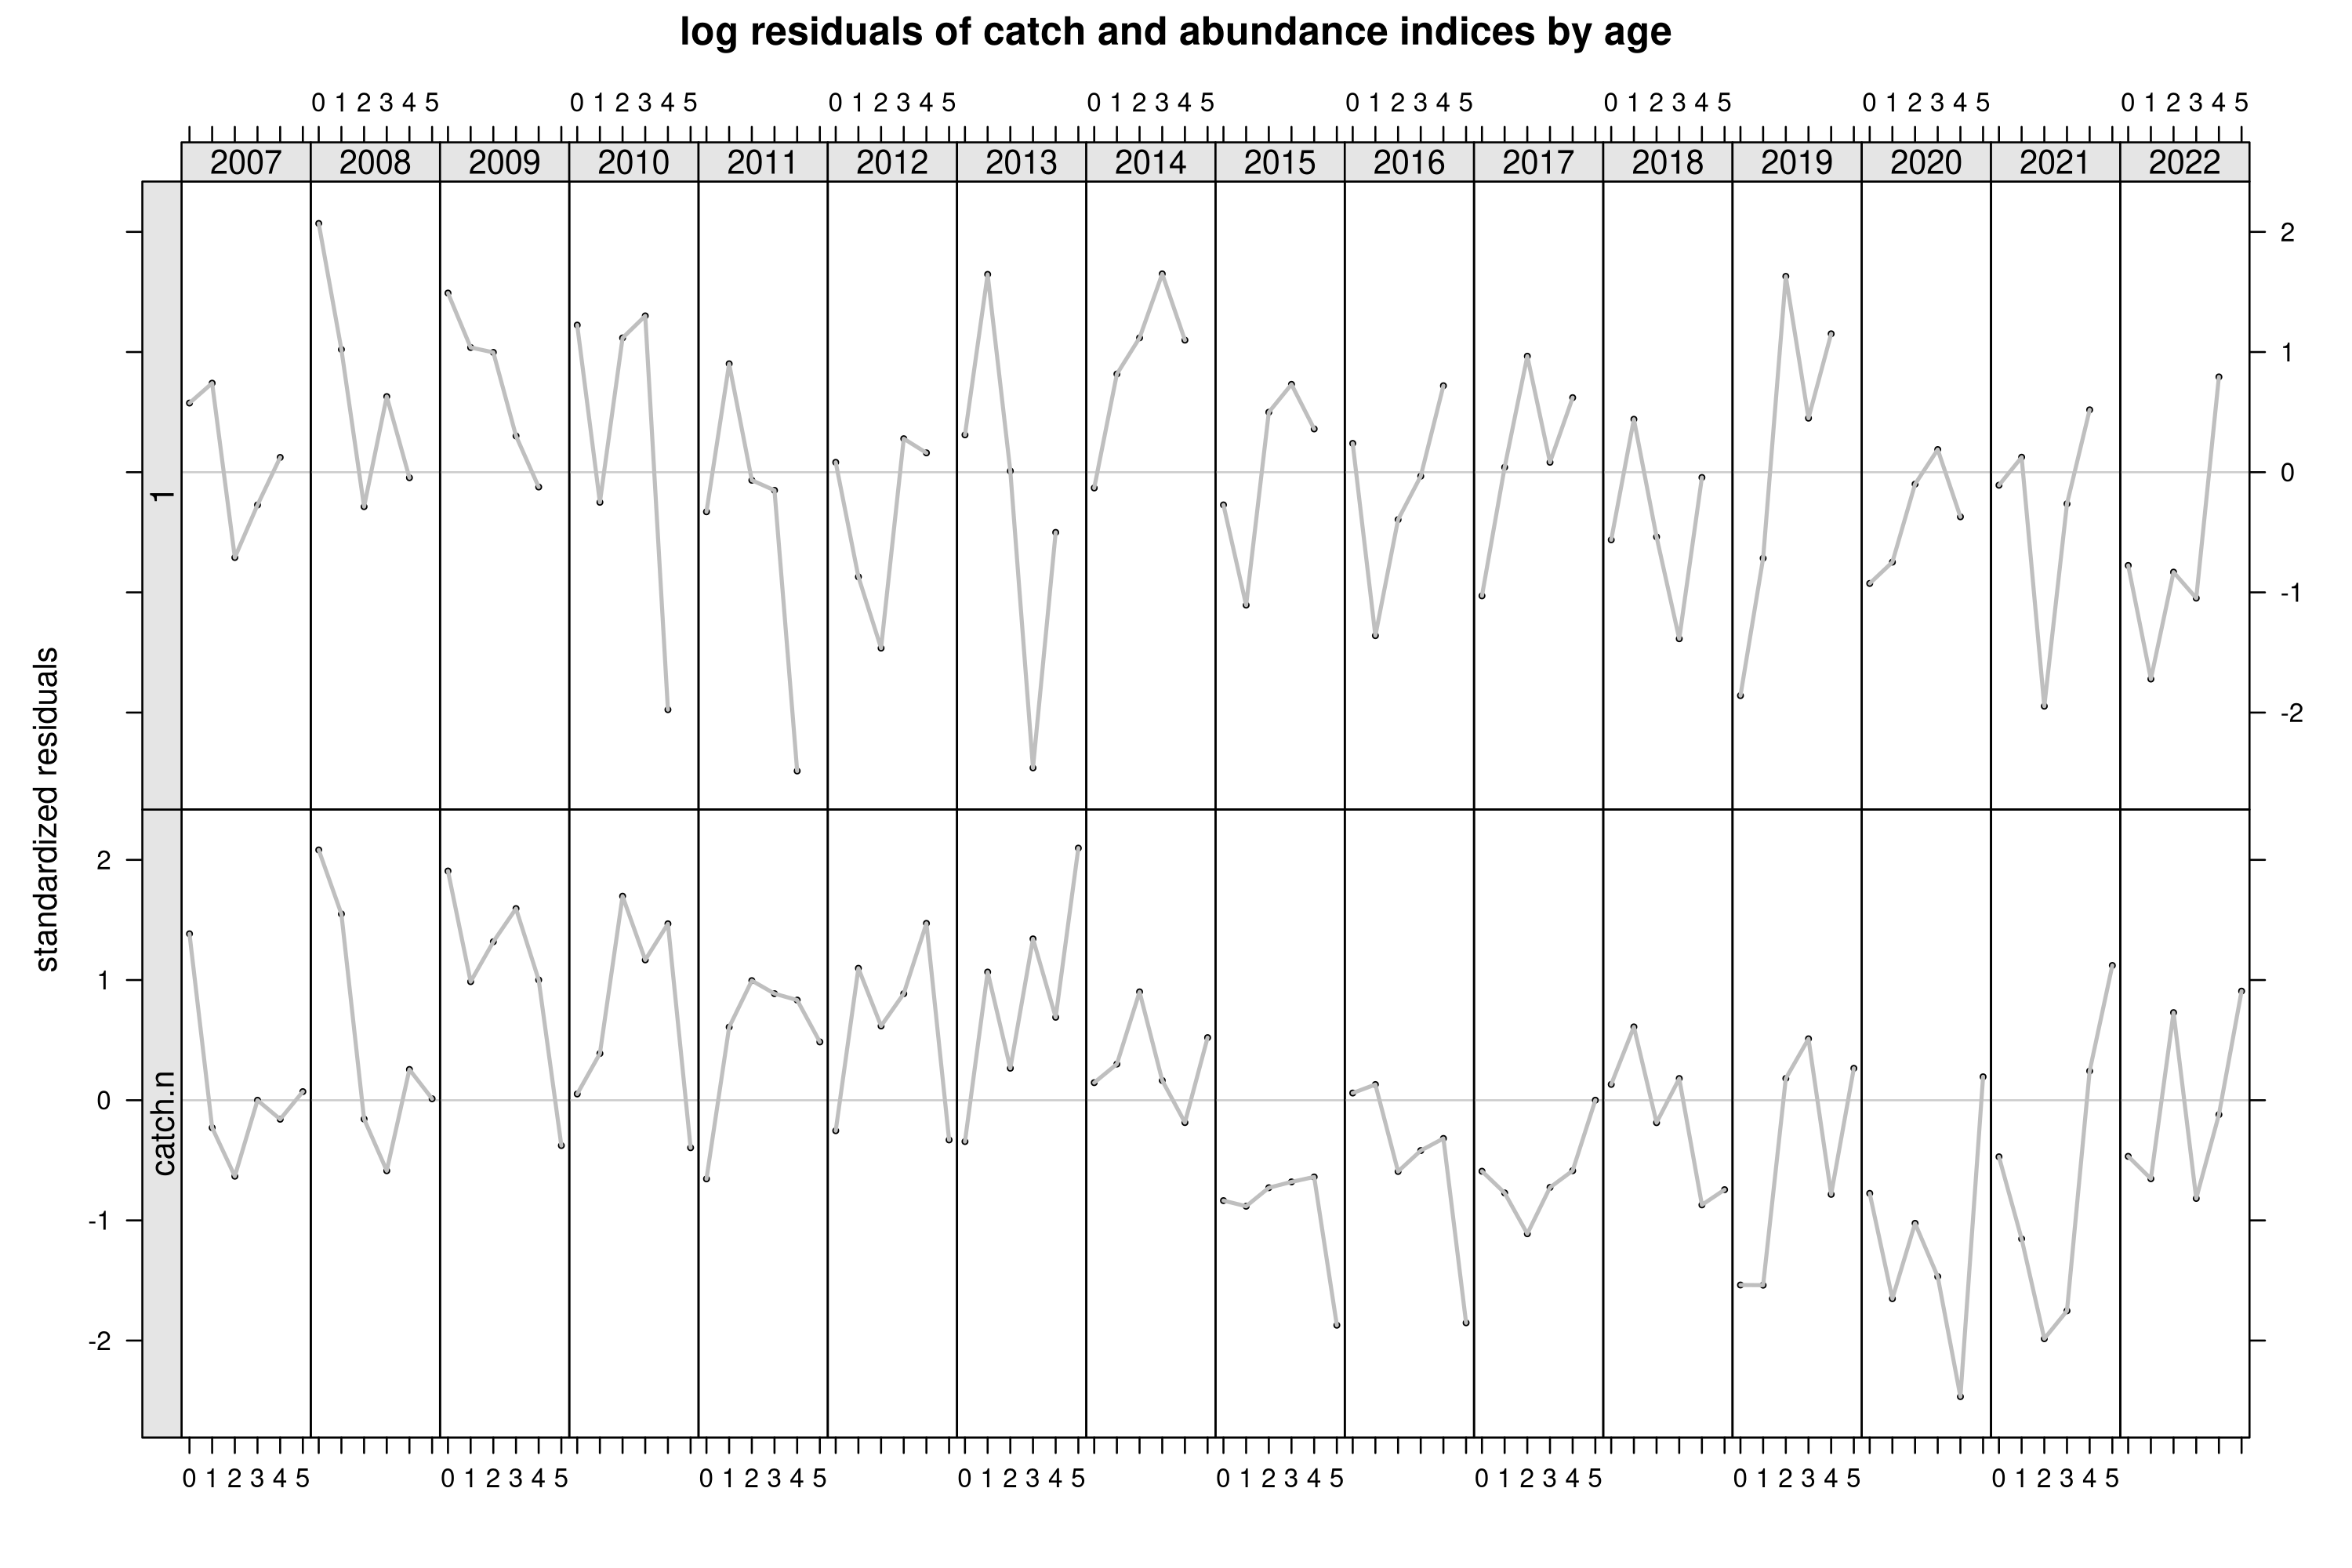
\includegraphics[width=25cm,height=18cm,angle=90]{figure/n1resbyage-1} 

}

\caption[f year effect fit residuals by age)]{f year effect fit residuals by age)}\label{fig:n1resbyage}
\end{figure}

\end{knitrout}

\subsection{The stock recruitment submodel }

There's a lot to say about this submodel (check the \aFa manual for more). In this example we'll simply add a model to allow recruitment to vary over time and we'll see how to track potential improvements in the residuals.

\begin{knitrout}
\definecolor{shadecolor}{rgb}{0.949, 0.949, 0.949}\color{fgcolor}\begin{kframe}
\begin{alltt}
\hldef{fit07} \hlkwb{<-} \hlkwd{sca}\hldef{(hke1567, hke1567.idx,} \hlkwc{fmod} \hldef{=} \hlopt{~}\hlkwd{factor}\hldef{(age)} \hlopt{+} \hlkwd{factor}\hldef{(year),} \hlkwc{qmod} \hldef{=} \hlkwd{list}\hldef{(}\hlopt{~}\hlkwd{factor}\hldef{(age)),}
    \hlkwc{srmod} \hldef{=} \hlopt{~}\hlkwd{factor}\hldef{(year),} \hlkwc{vmod} \hldef{=} \hlkwd{list}\hldef{(}\hlopt{~}\hlnum{1}\hldef{,} \hlopt{~}\hlnum{1}\hldef{),} \hlkwc{n1mod} \hldef{=} \hlopt{~}\hlkwd{factor}\hldef{(age))}
\hldef{res07} \hlkwb{<-} \hlkwd{residuals}\hldef{(fit07, hke1567, hke1567.idx)}
\end{alltt}
\end{kframe}
\end{knitrout}

The residuals plot by year are very useful to see the effect of adding a varying stock recruitment model. The year trends present in previous models are not absent. Recruitment variability when left unmodelled was being picked up by trends in the survey catchability and catch at age. And due to the cohort dynamics underlying the catch at age model, where propagating into other ages' estimates. 

\begin{knitrout}
\definecolor{shadecolor}{rgb}{0.949, 0.949, 0.949}\color{fgcolor}\begin{kframe}
\begin{alltt}
\hlkwd{plot}\hldef{(res07)}
\end{alltt}
\end{kframe}\begin{figure}[H]

{\centering 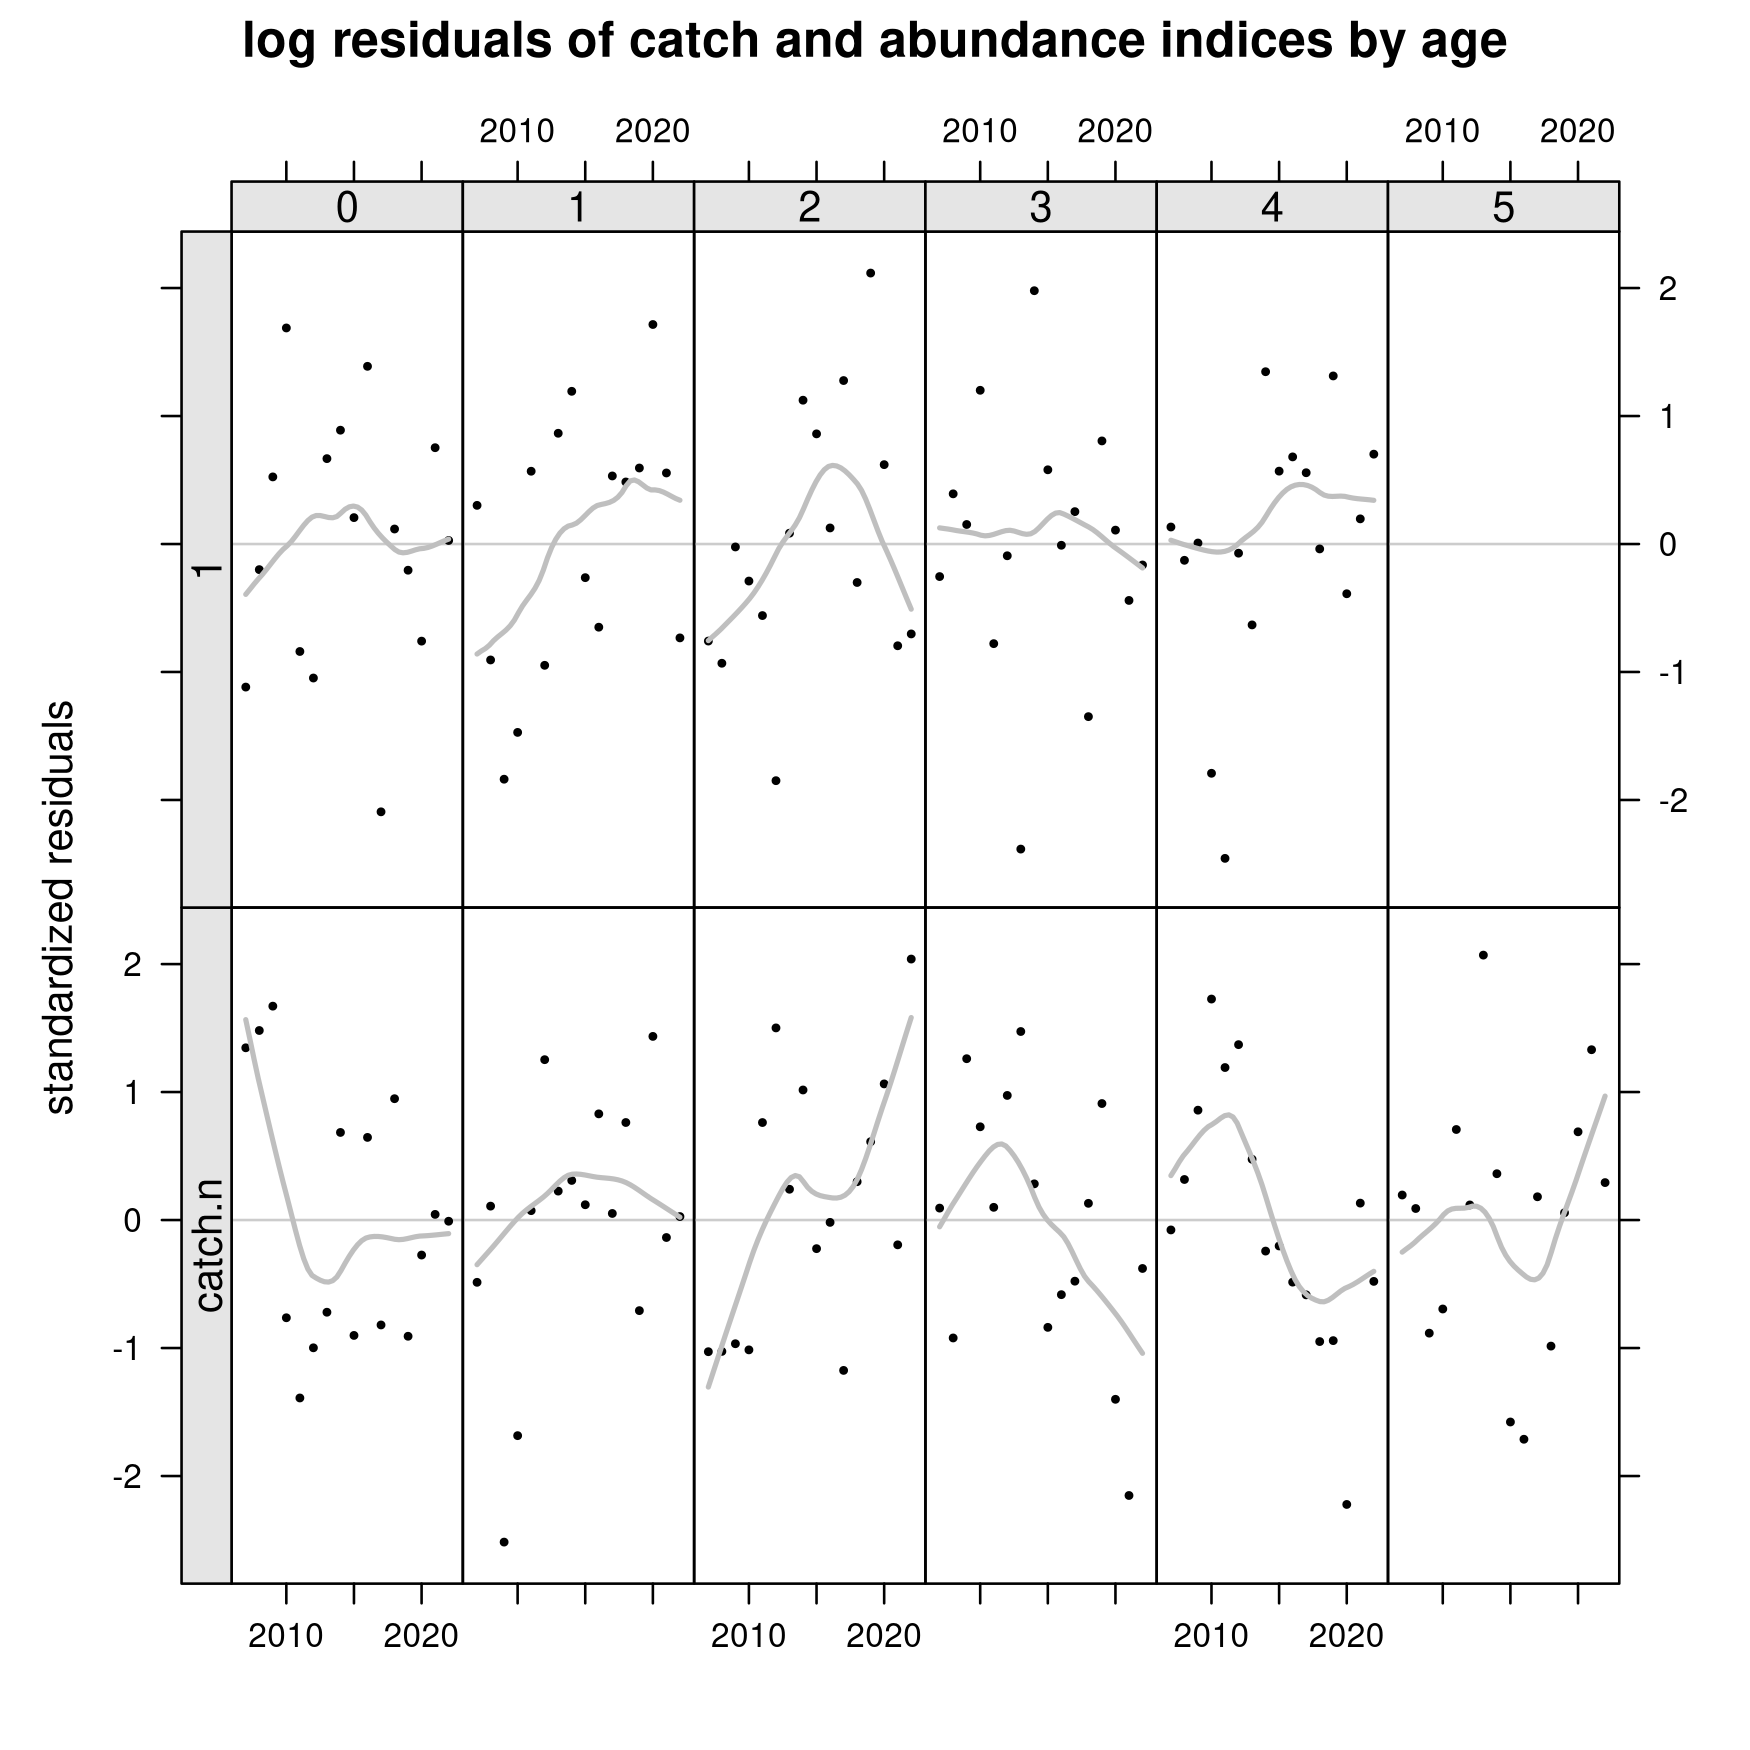
\includegraphics[width=.9\linewidth]{figure/srresbyyear-1} 

}

\caption[f year effect fit residuals by year)]{f year effect fit residuals by year)}\label{fig:srresbyyear}
\end{figure}

\end{knitrout}

\begin{knitrout}
\definecolor{shadecolor}{rgb}{0.949, 0.949, 0.949}\color{fgcolor}\begin{kframe}
\begin{alltt}
\hlkwd{plot}\hldef{(res07,} \hlkwc{auxline} \hldef{=} \hlsng{"l"}\hldef{,} \hlkwc{by} \hldef{=} \hlsng{"age"}\hldef{)}
\end{alltt}
\end{kframe}\begin{figure}[H]

{\centering 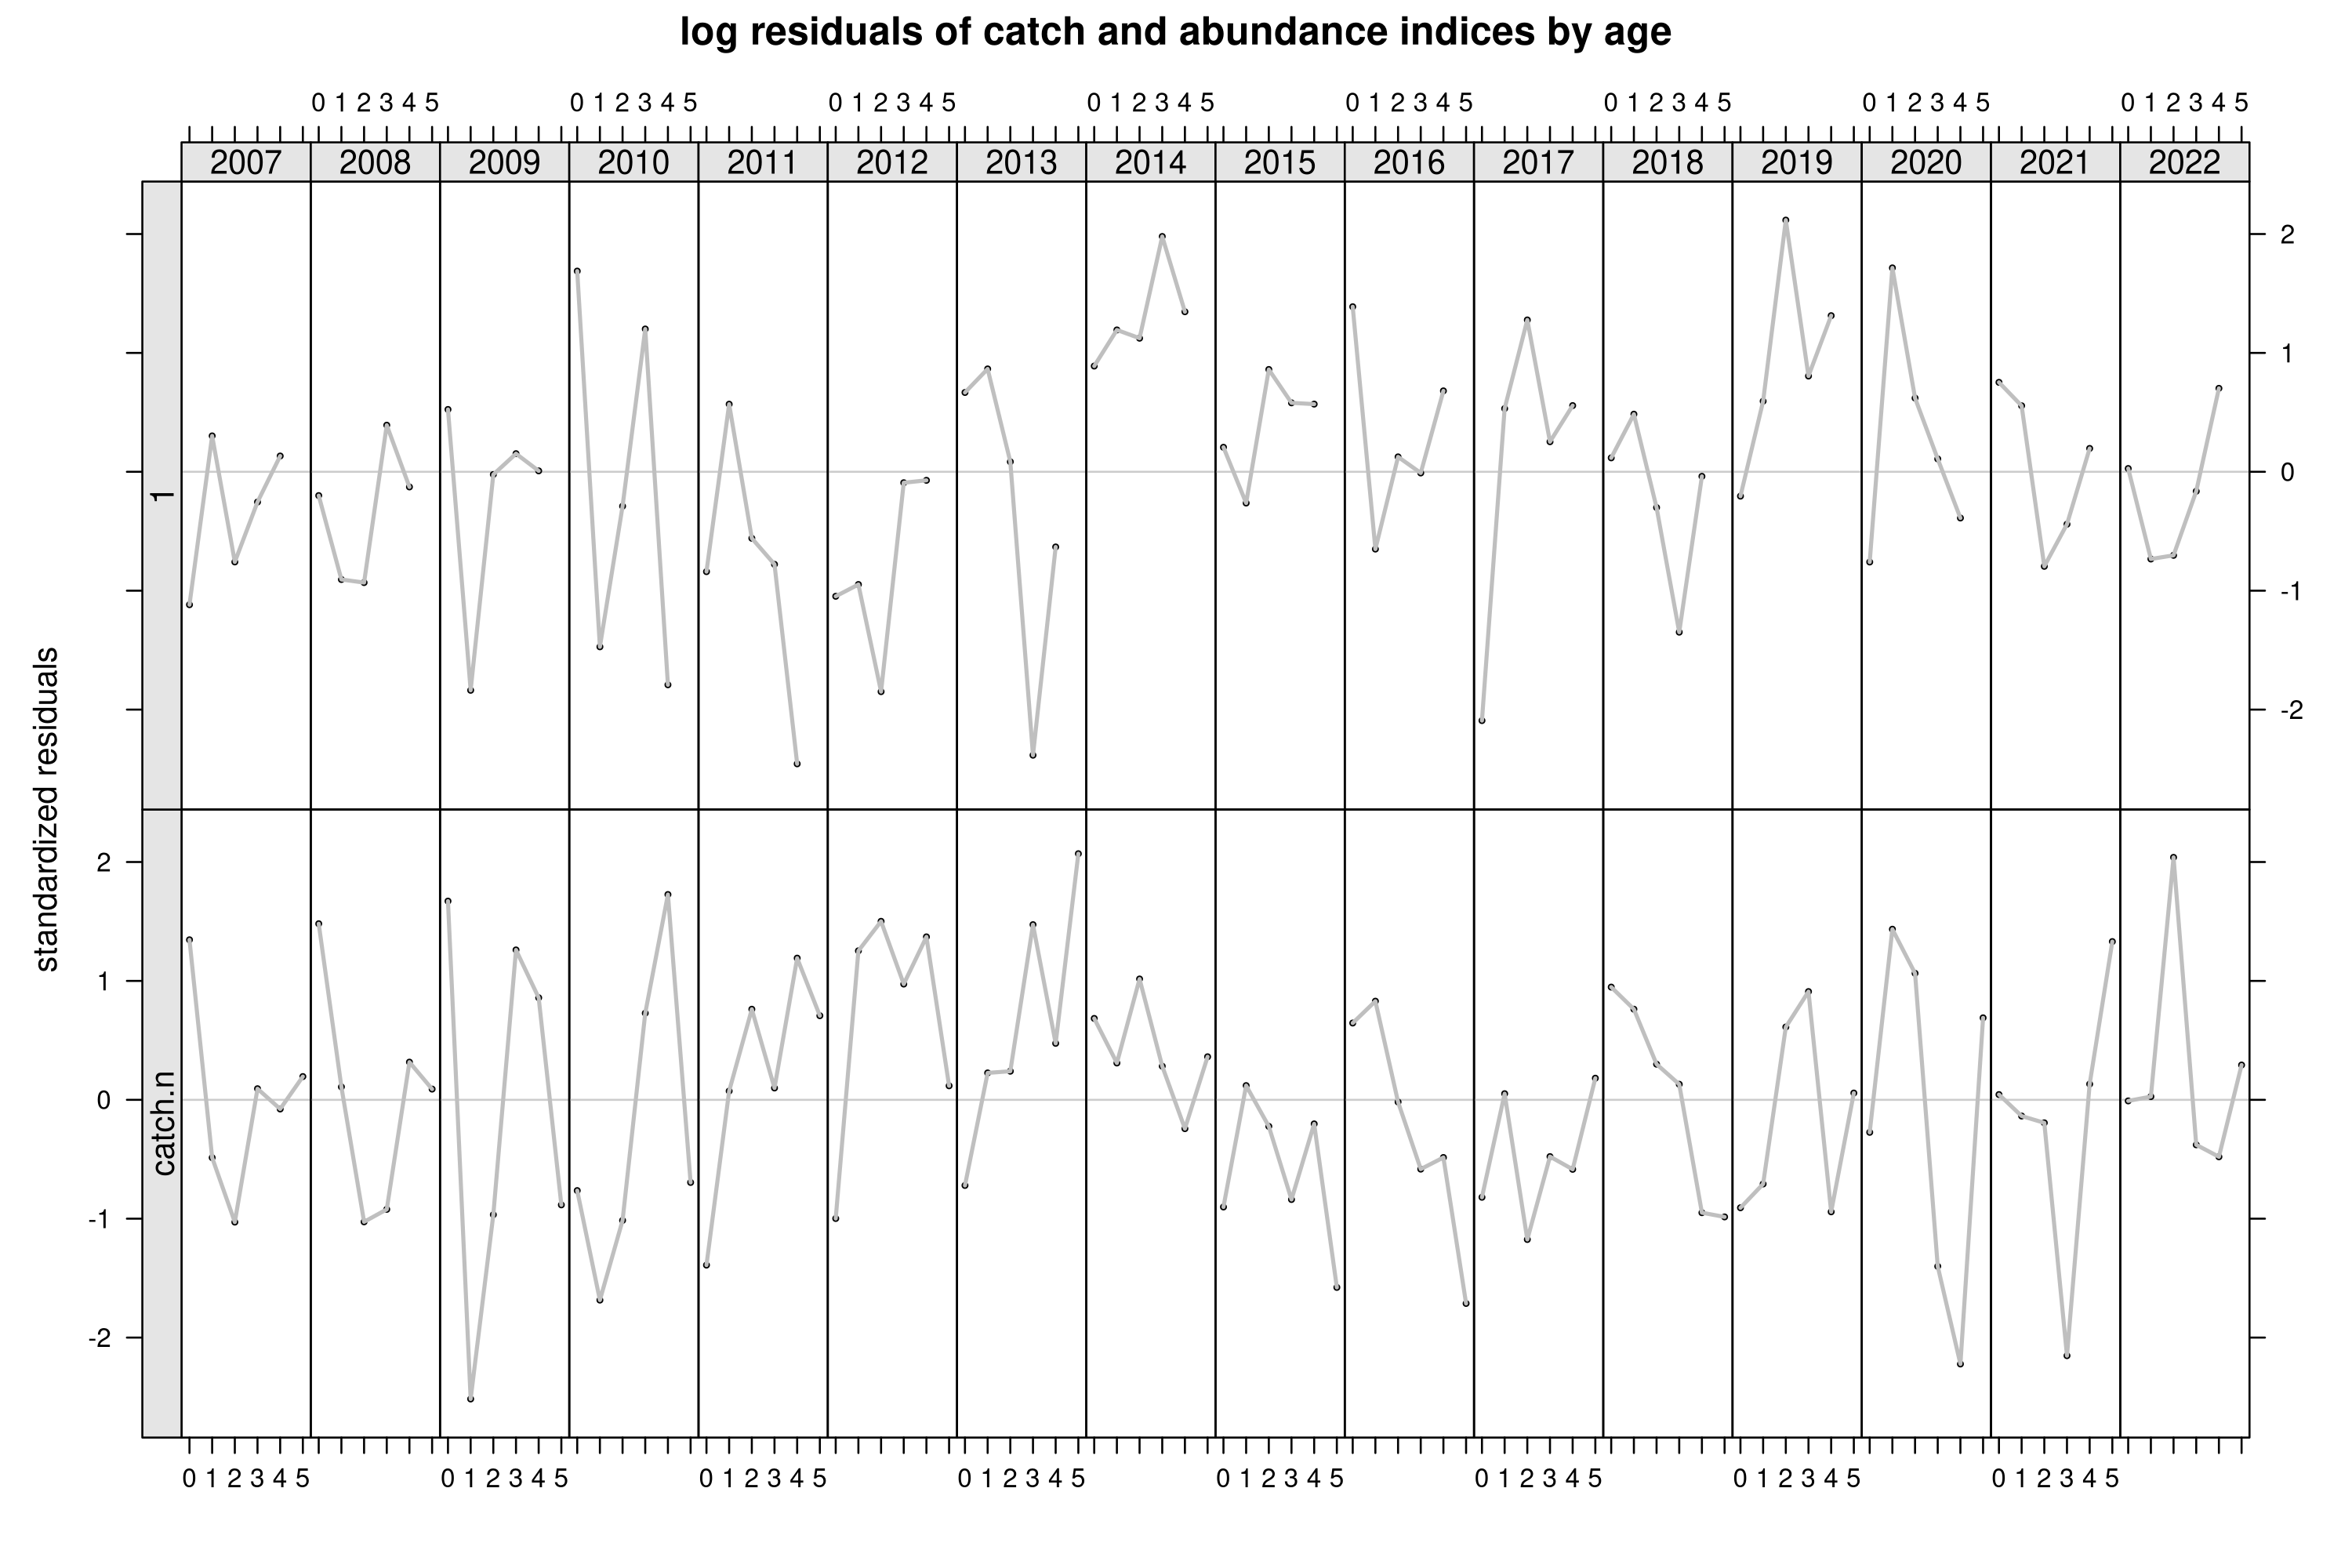
\includegraphics[width=25cm,height=18cm,angle=90]{figure/srresbyage-1} 

}

\caption[f year effect fit residuals by age)]{f year effect fit residuals by age)}\label{fig:srresbyage}
\end{figure}

\end{knitrout}

\subsection{Reducing the number of parameters}

In this section we'll look into how to use smoothers to reduce the number of parameters of the model. The process is laid out line by line but it could easily be wrapped in a function call to compute a BIC profile.

Due to the number of ages in the data, 4, and the minimum degrees of freedom one can use in a \code{MGCV} smoother, 3, there's not a lot to gain by playing with age effects. Our first attempt will be with both year effects, in fishing mortality and stock recruitment. Starting with a sparser vector of ks and later focusing in the region of minimal BIC.  

\begin{knitrout}
\definecolor{shadecolor}{rgb}{0.949, 0.949, 0.949}\color{fgcolor}\begin{kframe}
\begin{alltt}
\hldef{fit08a} \hlkwb{<-} \hlkwd{sca}\hldef{(hke1567, hke1567.idx,} \hlkwc{fmod} \hldef{=} \hlopt{~}\hlkwd{factor}\hldef{(age)} \hlopt{+} \hlkwd{s}\hldef{(year,} \hlkwc{k} \hldef{=} \hlnum{15}\hldef{),} \hlkwc{qmod} \hldef{=} \hlkwd{list}\hldef{(}\hlopt{~}\hlkwd{factor}\hldef{(age)),}
    \hlkwc{srmod} \hldef{=} \hlopt{~}\hlkwd{factor}\hldef{(year),} \hlkwc{vmod} \hldef{=} \hlkwd{list}\hldef{(}\hlopt{~}\hlnum{1}\hldef{,} \hlopt{~}\hlnum{1}\hldef{),} \hlkwc{n1mod} \hldef{=} \hlopt{~}\hlkwd{factor}\hldef{(age))}
\hldef{fit08b} \hlkwb{<-} \hlkwd{sca}\hldef{(hke1567, hke1567.idx,} \hlkwc{fmod} \hldef{=} \hlopt{~}\hlkwd{factor}\hldef{(age)} \hlopt{+} \hlkwd{s}\hldef{(year,} \hlkwc{k} \hldef{=} \hlnum{10}\hldef{),} \hlkwc{qmod} \hldef{=} \hlkwd{list}\hldef{(}\hlopt{~}\hlkwd{factor}\hldef{(age)),}
    \hlkwc{srmod} \hldef{=} \hlopt{~}\hlkwd{factor}\hldef{(year),} \hlkwc{vmod} \hldef{=} \hlkwd{list}\hldef{(}\hlopt{~}\hlnum{1}\hldef{,} \hlopt{~}\hlnum{1}\hldef{),} \hlkwc{n1mod} \hldef{=} \hlopt{~}\hlkwd{factor}\hldef{(age))}
\hldef{fit08c} \hlkwb{<-} \hlkwd{sca}\hldef{(hke1567, hke1567.idx,} \hlkwc{fmod} \hldef{=} \hlopt{~}\hlkwd{factor}\hldef{(age)} \hlopt{+} \hlkwd{s}\hldef{(year,} \hlkwc{k} \hldef{=} \hlnum{5}\hldef{),} \hlkwc{qmod} \hldef{=} \hlkwd{list}\hldef{(}\hlopt{~}\hlkwd{factor}\hldef{(age)),}
    \hlkwc{srmod} \hldef{=} \hlopt{~}\hlkwd{factor}\hldef{(year),} \hlkwc{vmod} \hldef{=} \hlkwd{list}\hldef{(}\hlopt{~}\hlnum{1}\hldef{,} \hlopt{~}\hlnum{1}\hldef{),} \hlkwc{n1mod} \hldef{=} \hlopt{~}\hlkwd{factor}\hldef{(age))}

\hlkwd{BIC}\hldef{(fit08a, fit08b, fit08c)}
\end{alltt}
\begin{verbatim}
##        df      BIC
## fit08a 48 438.9668
## fit08b 43 418.8915
## fit08c 38 403.6692
\end{verbatim}
\begin{alltt}
\hldef{fit08d} \hlkwb{<-} \hlkwd{sca}\hldef{(hke1567, hke1567.idx,} \hlkwc{fmod} \hldef{=} \hlopt{~}\hlkwd{factor}\hldef{(age)} \hlopt{+} \hlkwd{s}\hldef{(year,} \hlkwc{k} \hldef{=} \hlnum{7}\hldef{),} \hlkwc{qmod} \hldef{=} \hlkwd{list}\hldef{(}\hlopt{~}\hlkwd{factor}\hldef{(age)),}
    \hlkwc{srmod} \hldef{=} \hlopt{~}\hlkwd{factor}\hldef{(year),} \hlkwc{vmod} \hldef{=} \hlkwd{list}\hldef{(}\hlopt{~}\hlnum{1}\hldef{,} \hlopt{~}\hlnum{1}\hldef{),} \hlkwc{n1mod} \hldef{=} \hlopt{~}\hlkwd{factor}\hldef{(age))}
\hldef{fit08e} \hlkwb{<-} \hlkwd{sca}\hldef{(hke1567, hke1567.idx,} \hlkwc{fmod} \hldef{=} \hlopt{~}\hlkwd{factor}\hldef{(age)} \hlopt{+} \hlkwd{s}\hldef{(year,} \hlkwc{k} \hldef{=} \hlnum{6}\hldef{),} \hlkwc{qmod} \hldef{=} \hlkwd{list}\hldef{(}\hlopt{~}\hlkwd{factor}\hldef{(age)),}
    \hlkwc{srmod} \hldef{=} \hlopt{~}\hlkwd{factor}\hldef{(year),} \hlkwc{vmod} \hldef{=} \hlkwd{list}\hldef{(}\hlopt{~}\hlnum{1}\hldef{,} \hlopt{~}\hlnum{1}\hldef{),} \hlkwc{n1mod} \hldef{=} \hlopt{~}\hlkwd{factor}\hldef{(age))}
\hldef{fit08f} \hlkwb{<-} \hlkwd{sca}\hldef{(hke1567, hke1567.idx,} \hlkwc{fmod} \hldef{=} \hlopt{~}\hlkwd{factor}\hldef{(age)} \hlopt{+} \hlkwd{s}\hldef{(year,} \hlkwc{k} \hldef{=} \hlnum{4}\hldef{),} \hlkwc{qmod} \hldef{=} \hlkwd{list}\hldef{(}\hlopt{~}\hlkwd{factor}\hldef{(age)),}
    \hlkwc{srmod} \hldef{=} \hlopt{~}\hlkwd{factor}\hldef{(year),} \hlkwc{vmod} \hldef{=} \hlkwd{list}\hldef{(}\hlopt{~}\hlnum{1}\hldef{,} \hlopt{~}\hlnum{1}\hldef{),} \hlkwc{n1mod} \hldef{=} \hlopt{~}\hlkwd{factor}\hldef{(age))}
\hldef{fit08g} \hlkwb{<-} \hlkwd{sca}\hldef{(hke1567, hke1567.idx,} \hlkwc{fmod} \hldef{=} \hlopt{~}\hlkwd{factor}\hldef{(age)} \hlopt{+} \hlkwd{s}\hldef{(year,} \hlkwc{k} \hldef{=} \hlnum{3}\hldef{),} \hlkwc{qmod} \hldef{=} \hlkwd{list}\hldef{(}\hlopt{~}\hlkwd{factor}\hldef{(age)),}
    \hlkwc{srmod} \hldef{=} \hlopt{~}\hlkwd{factor}\hldef{(year),} \hlkwc{vmod} \hldef{=} \hlkwd{list}\hldef{(}\hlopt{~}\hlnum{1}\hldef{,} \hlopt{~}\hlnum{1}\hldef{),} \hlkwc{n1mod} \hldef{=} \hlopt{~}\hlkwd{factor}\hldef{(age))}

\hlkwd{BIC}\hldef{(fit08a, fit08b, fit08c, fit08d, fit08e, fit08f, fit08g)}
\end{alltt}
\begin{verbatim}
##        df      BIC
## fit08a 48 438.9668
## fit08b 43 418.8915
## fit08c 38 403.6692
## fit08d 40 408.9315
## fit08e 39 405.1384
## fit08f 37 406.8219
## fit08g 36 402.2597
\end{verbatim}
\end{kframe}
\end{knitrout}

Using \code{k = 5} is the best option if using BIC for comparison.

\begin{knitrout}
\definecolor{shadecolor}{rgb}{0.949, 0.949, 0.949}\color{fgcolor}\begin{kframe}
\begin{alltt}
\hldef{fit08} \hlkwb{<-} \hlkwd{sca}\hldef{(hke1567, hke1567.idx,} \hlkwc{fmod} \hldef{=} \hlopt{~}\hlkwd{factor}\hldef{(age)} \hlopt{+} \hlkwd{s}\hldef{(year,} \hlkwc{k} \hldef{=} \hlnum{5}\hldef{),} \hlkwc{qmod} \hldef{=} \hlkwd{list}\hldef{(}\hlopt{~}\hlkwd{factor}\hldef{(age)),}
    \hlkwc{srmod} \hldef{=} \hlopt{~}\hlkwd{factor}\hldef{(year),} \hlkwc{vmod} \hldef{=} \hlkwd{list}\hldef{(}\hlopt{~}\hlnum{1}\hldef{,} \hlopt{~}\hlnum{1}\hldef{),} \hlkwc{n1mod} \hldef{=} \hlopt{~}\hlkwd{factor}\hldef{(age))}
\hldef{res08} \hlkwb{<-} \hlkwd{residuals}\hldef{(fit08, hke1567, hke1567.idx)}
\end{alltt}
\end{kframe}
\end{knitrout}

\begin{knitrout}
\definecolor{shadecolor}{rgb}{0.949, 0.949, 0.949}\color{fgcolor}\begin{kframe}
\begin{alltt}
\hlkwd{plot}\hldef{(res08)}
\end{alltt}
\end{kframe}\begin{figure}[H]

{\centering 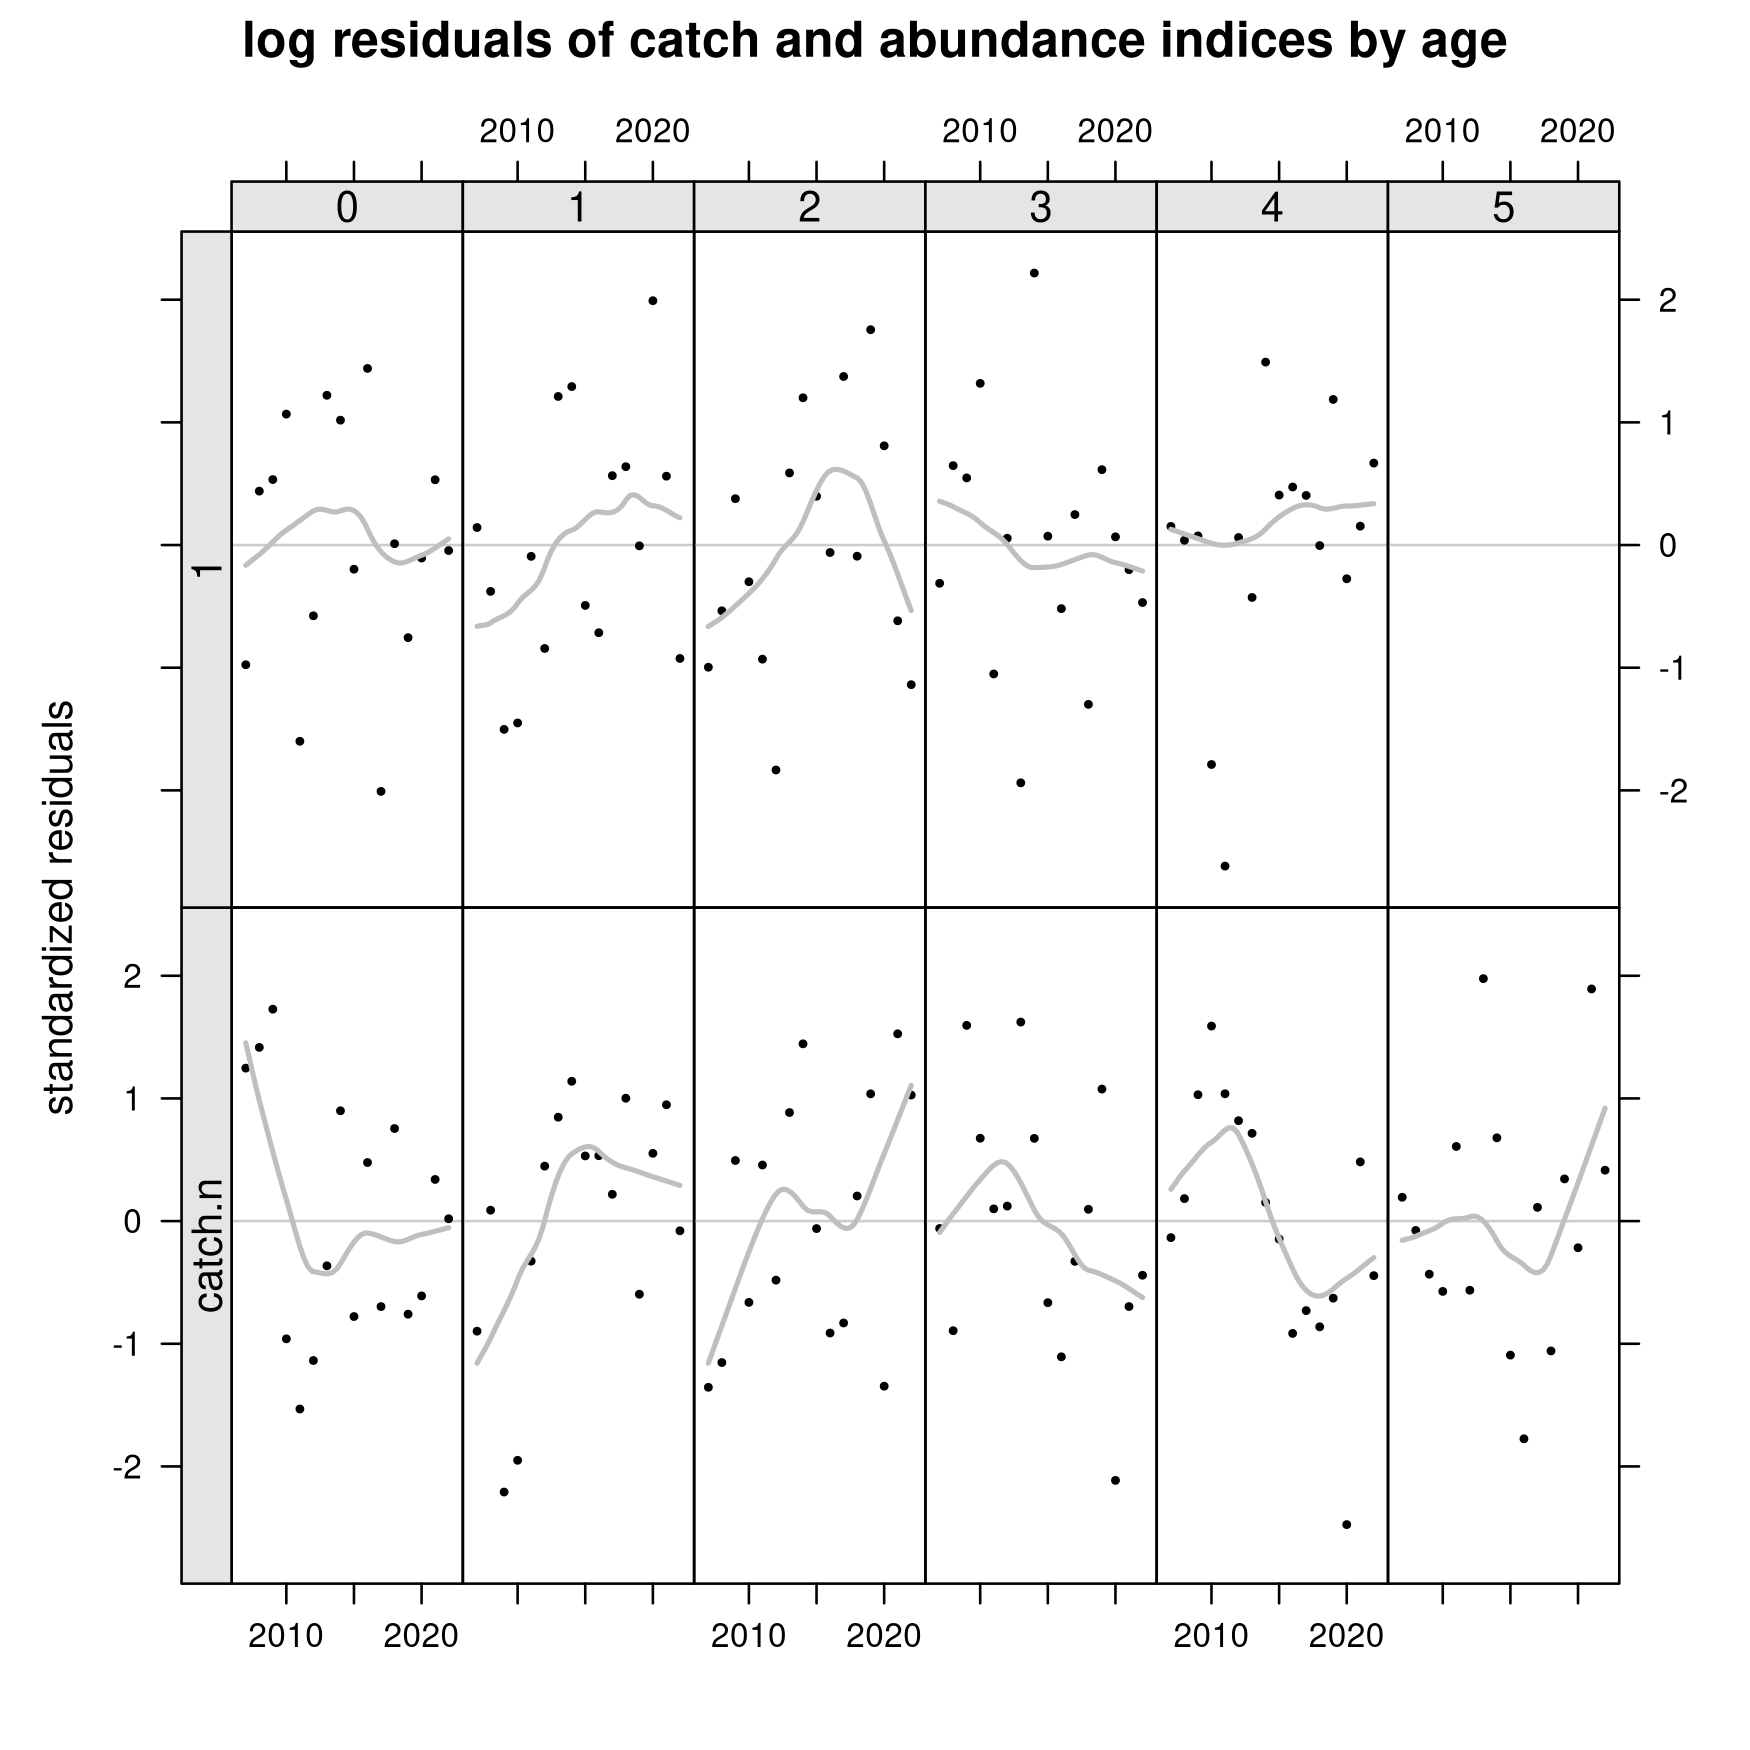
\includegraphics[width=.9\linewidth]{figure/fksresbyyear-1} 

}

\caption[f year effect fit residuals by year)]{f year effect fit residuals by year)}\label{fig:fksresbyyear}
\end{figure}

\end{knitrout}

\begin{knitrout}
\definecolor{shadecolor}{rgb}{0.949, 0.949, 0.949}\color{fgcolor}\begin{kframe}
\begin{alltt}
\hlkwd{plot}\hldef{(res08,} \hlkwc{auxline} \hldef{=} \hlsng{"l"}\hldef{,} \hlkwc{by} \hldef{=} \hlsng{"age"}\hldef{)}
\end{alltt}
\end{kframe}\begin{figure}[H]

{\centering 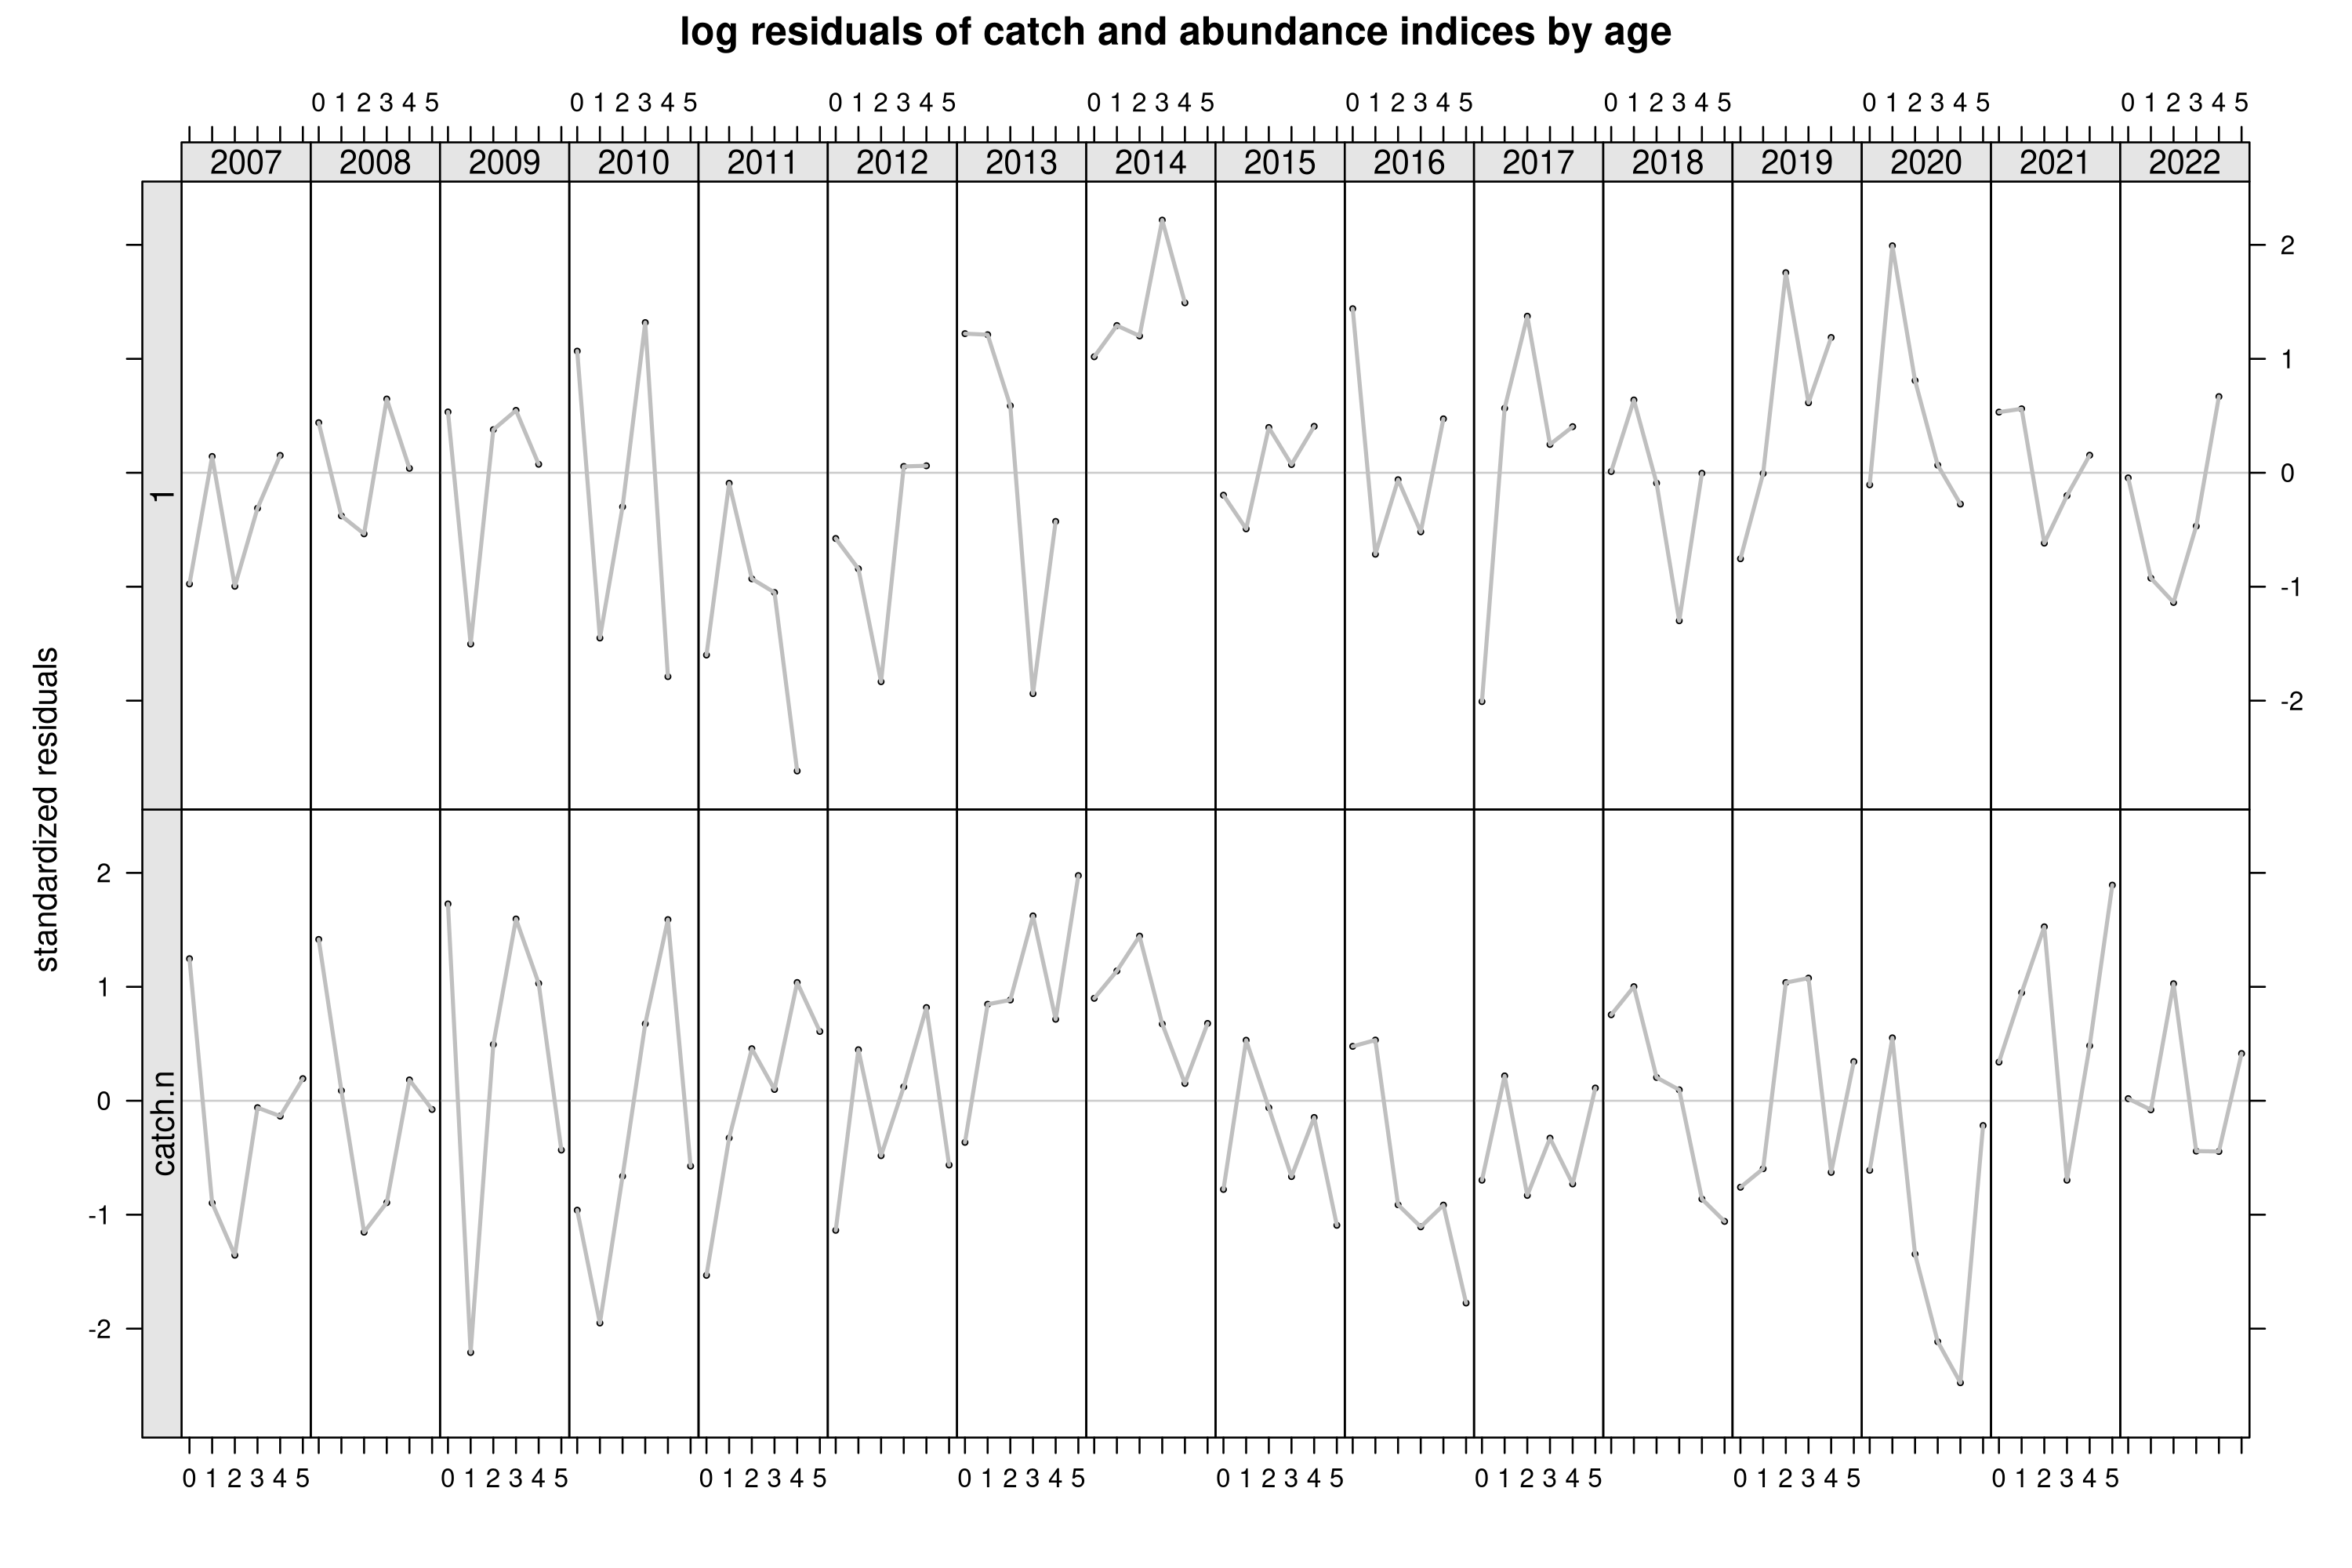
\includegraphics[width=25cm,height=18cm,angle=90]{figure/fksresbyage-1} 

}

\caption[f year effect fit residuals by age)]{f year effect fit residuals by age)}\label{fig:fksresbyage}
\end{figure}

\end{knitrout}

Following the same approach let's check what can be done with regards to the recruitment model degrees of freedom.

\begin{knitrout}
\definecolor{shadecolor}{rgb}{0.949, 0.949, 0.949}\color{fgcolor}\begin{kframe}
\begin{alltt}
\hldef{fit09a} \hlkwb{<-} \hlkwd{sca}\hldef{(hke1567, hke1567.idx,} \hlkwc{fmod} \hldef{=} \hlopt{~}\hlkwd{factor}\hldef{(age)} \hlopt{+} \hlkwd{s}\hldef{(year,} \hlkwc{k} \hldef{=} \hlnum{5}\hldef{),} \hlkwc{qmod} \hldef{=} \hlkwd{list}\hldef{(}\hlopt{~}\hlkwd{factor}\hldef{(age)),}
    \hlkwc{srmod} \hldef{=} \hlopt{~}\hlkwd{s}\hldef{(year,} \hlkwc{k} \hldef{=} \hlnum{15}\hldef{),} \hlkwc{vmod} \hldef{=} \hlkwd{list}\hldef{(}\hlopt{~}\hlnum{1}\hldef{,} \hlopt{~}\hlnum{1}\hldef{),} \hlkwc{n1mod} \hldef{=} \hlopt{~}\hlkwd{factor}\hldef{(age))}
\hldef{fit09b} \hlkwb{<-} \hlkwd{sca}\hldef{(hke1567, hke1567.idx,} \hlkwc{fmod} \hldef{=} \hlopt{~}\hlkwd{factor}\hldef{(age)} \hlopt{+} \hlkwd{s}\hldef{(year,} \hlkwc{k} \hldef{=} \hlnum{5}\hldef{),} \hlkwc{qmod} \hldef{=} \hlkwd{list}\hldef{(}\hlopt{~}\hlkwd{factor}\hldef{(age)),}
    \hlkwc{srmod} \hldef{=} \hlopt{~}\hlkwd{s}\hldef{(year,} \hlkwc{k} \hldef{=} \hlnum{10}\hldef{),} \hlkwc{vmod} \hldef{=} \hlkwd{list}\hldef{(}\hlopt{~}\hlnum{1}\hldef{,} \hlopt{~}\hlnum{1}\hldef{),} \hlkwc{n1mod} \hldef{=} \hlopt{~}\hlkwd{factor}\hldef{(age))}
\hldef{fit09c} \hlkwb{<-} \hlkwd{sca}\hldef{(hke1567, hke1567.idx,} \hlkwc{fmod} \hldef{=} \hlopt{~}\hlkwd{factor}\hldef{(age)} \hlopt{+} \hlkwd{s}\hldef{(year,} \hlkwc{k} \hldef{=} \hlnum{5}\hldef{),} \hlkwc{qmod} \hldef{=} \hlkwd{list}\hldef{(}\hlopt{~}\hlkwd{factor}\hldef{(age)),}
    \hlkwc{srmod} \hldef{=} \hlopt{~}\hlkwd{s}\hldef{(year,} \hlkwc{k} \hldef{=} \hlnum{5}\hldef{),} \hlkwc{vmod} \hldef{=} \hlkwd{list}\hldef{(}\hlopt{~}\hlnum{1}\hldef{,} \hlopt{~}\hlnum{1}\hldef{),} \hlkwc{n1mod} \hldef{=} \hlopt{~}\hlkwd{factor}\hldef{(age))}

\hlkwd{BIC}\hldef{(fit09a, fit09b, fit09c)}
\end{alltt}
\begin{verbatim}
##        df      BIC
## fit09a 37 398.5131
## fit09b 32 378.9776
## fit09c 27 365.2791
\end{verbatim}
\begin{alltt}
\hldef{fit09d} \hlkwb{<-} \hlkwd{sca}\hldef{(hke1567, hke1567.idx,} \hlkwc{fmod} \hldef{=} \hlopt{~}\hlkwd{factor}\hldef{(age)} \hlopt{+} \hlkwd{s}\hldef{(year,} \hlkwc{k} \hldef{=} \hlnum{5}\hldef{),} \hlkwc{qmod} \hldef{=} \hlkwd{list}\hldef{(}\hlopt{~}\hlkwd{factor}\hldef{(age)),}
    \hlkwc{srmod} \hldef{=} \hlopt{~}\hlkwd{s}\hldef{(year,} \hlkwc{k} \hldef{=} \hlnum{7}\hldef{),} \hlkwc{vmod} \hldef{=} \hlkwd{list}\hldef{(}\hlopt{~}\hlnum{1}\hldef{,} \hlopt{~}\hlnum{1}\hldef{),} \hlkwc{n1mod} \hldef{=} \hlopt{~}\hlkwd{factor}\hldef{(age))}
\hldef{fit09e} \hlkwb{<-} \hlkwd{sca}\hldef{(hke1567, hke1567.idx,} \hlkwc{fmod} \hldef{=} \hlopt{~}\hlkwd{factor}\hldef{(age)} \hlopt{+} \hlkwd{s}\hldef{(year,} \hlkwc{k} \hldef{=} \hlnum{5}\hldef{),} \hlkwc{qmod} \hldef{=} \hlkwd{list}\hldef{(}\hlopt{~}\hlkwd{factor}\hldef{(age)),}
    \hlkwc{srmod} \hldef{=} \hlopt{~}\hlkwd{s}\hldef{(year,} \hlkwc{k} \hldef{=} \hlnum{6}\hldef{),} \hlkwc{vmod} \hldef{=} \hlkwd{list}\hldef{(}\hlopt{~}\hlnum{1}\hldef{,} \hlopt{~}\hlnum{1}\hldef{),} \hlkwc{n1mod} \hldef{=} \hlopt{~}\hlkwd{factor}\hldef{(age))}
\hldef{fit09f} \hlkwb{<-} \hlkwd{sca}\hldef{(hke1567, hke1567.idx,} \hlkwc{fmod} \hldef{=} \hlopt{~}\hlkwd{factor}\hldef{(age)} \hlopt{+} \hlkwd{s}\hldef{(year,} \hlkwc{k} \hldef{=} \hlnum{5}\hldef{),} \hlkwc{qmod} \hldef{=} \hlkwd{list}\hldef{(}\hlopt{~}\hlkwd{factor}\hldef{(age)),}
    \hlkwc{srmod} \hldef{=} \hlopt{~}\hlkwd{s}\hldef{(year,} \hlkwc{k} \hldef{=} \hlnum{4}\hldef{),} \hlkwc{vmod} \hldef{=} \hlkwd{list}\hldef{(}\hlopt{~}\hlnum{1}\hldef{,} \hlopt{~}\hlnum{1}\hldef{),} \hlkwc{n1mod} \hldef{=} \hlopt{~}\hlkwd{factor}\hldef{(age))}
\hldef{fit09g} \hlkwb{<-} \hlkwd{sca}\hldef{(hke1567, hke1567.idx,} \hlkwc{fmod} \hldef{=} \hlopt{~}\hlkwd{factor}\hldef{(age)} \hlopt{+} \hlkwd{s}\hldef{(year,} \hlkwc{k} \hldef{=} \hlnum{5}\hldef{),} \hlkwc{qmod} \hldef{=} \hlkwd{list}\hldef{(}\hlopt{~}\hlkwd{factor}\hldef{(age)),}
    \hlkwc{srmod} \hldef{=} \hlopt{~}\hlkwd{s}\hldef{(year,} \hlkwc{k} \hldef{=} \hlnum{3}\hldef{),} \hlkwc{vmod} \hldef{=} \hlkwd{list}\hldef{(}\hlopt{~}\hlnum{1}\hldef{,} \hlopt{~}\hlnum{1}\hldef{),} \hlkwc{n1mod} \hldef{=} \hlopt{~}\hlkwd{factor}\hldef{(age))}

\hlkwd{BIC}\hldef{(fit09a, fit09b, fit09c, fit09d, fit09e, fit09f, fit09g)}
\end{alltt}
\begin{verbatim}
##        df      BIC
## fit09a 37 398.5131
## fit09b 32 378.9776
## fit09c 27 365.2791
## fit09d 29 370.3808
## fit09e 28 365.5614
## fit09f 26 360.5134
## fit09g 25 355.5995
\end{verbatim}
\end{kframe}
\end{knitrout}

The best model according to BIC is again \code{k = 5} for the recruitment submodel and as such the best model we get is:

\begin{knitrout}
\definecolor{shadecolor}{rgb}{0.949, 0.949, 0.949}\color{fgcolor}\begin{kframe}
\begin{alltt}
\hldef{fit09} \hlkwb{<-} \hlkwd{sca}\hldef{(hke1567, hke1567.idx,} \hlkwc{fmod} \hldef{=} \hlopt{~}\hlkwd{factor}\hldef{(age)} \hlopt{+} \hlkwd{s}\hldef{(year,} \hlkwc{k} \hldef{=} \hlnum{5}\hldef{),} \hlkwc{qmod} \hldef{=} \hlkwd{list}\hldef{(}\hlopt{~}\hlkwd{factor}\hldef{(age)),}
    \hlkwc{srmod} \hldef{=} \hlopt{~}\hlkwd{s}\hldef{(year,} \hlkwc{k} \hldef{=} \hlnum{5}\hldef{),} \hlkwc{vmod} \hldef{=} \hlkwd{list}\hldef{(}\hlopt{~}\hlnum{1}\hldef{,} \hlopt{~}\hlnum{1}\hldef{),} \hlkwc{n1mod} \hldef{=} \hlopt{~}\hlkwd{factor}\hldef{(age))}
\hldef{res09} \hlkwb{<-} \hlkwd{residuals}\hldef{(fit09, hke1567, hke1567.idx)}
\end{alltt}
\end{kframe}
\end{knitrout}

\begin{knitrout}
\definecolor{shadecolor}{rgb}{0.949, 0.949, 0.949}\color{fgcolor}\begin{kframe}
\begin{alltt}
\hlkwd{plot}\hldef{(res09,} \hlkwc{auxline} \hldef{=} \hlsng{"r"}\hldef{)}
\end{alltt}
\end{kframe}\begin{figure}[H]

{\centering 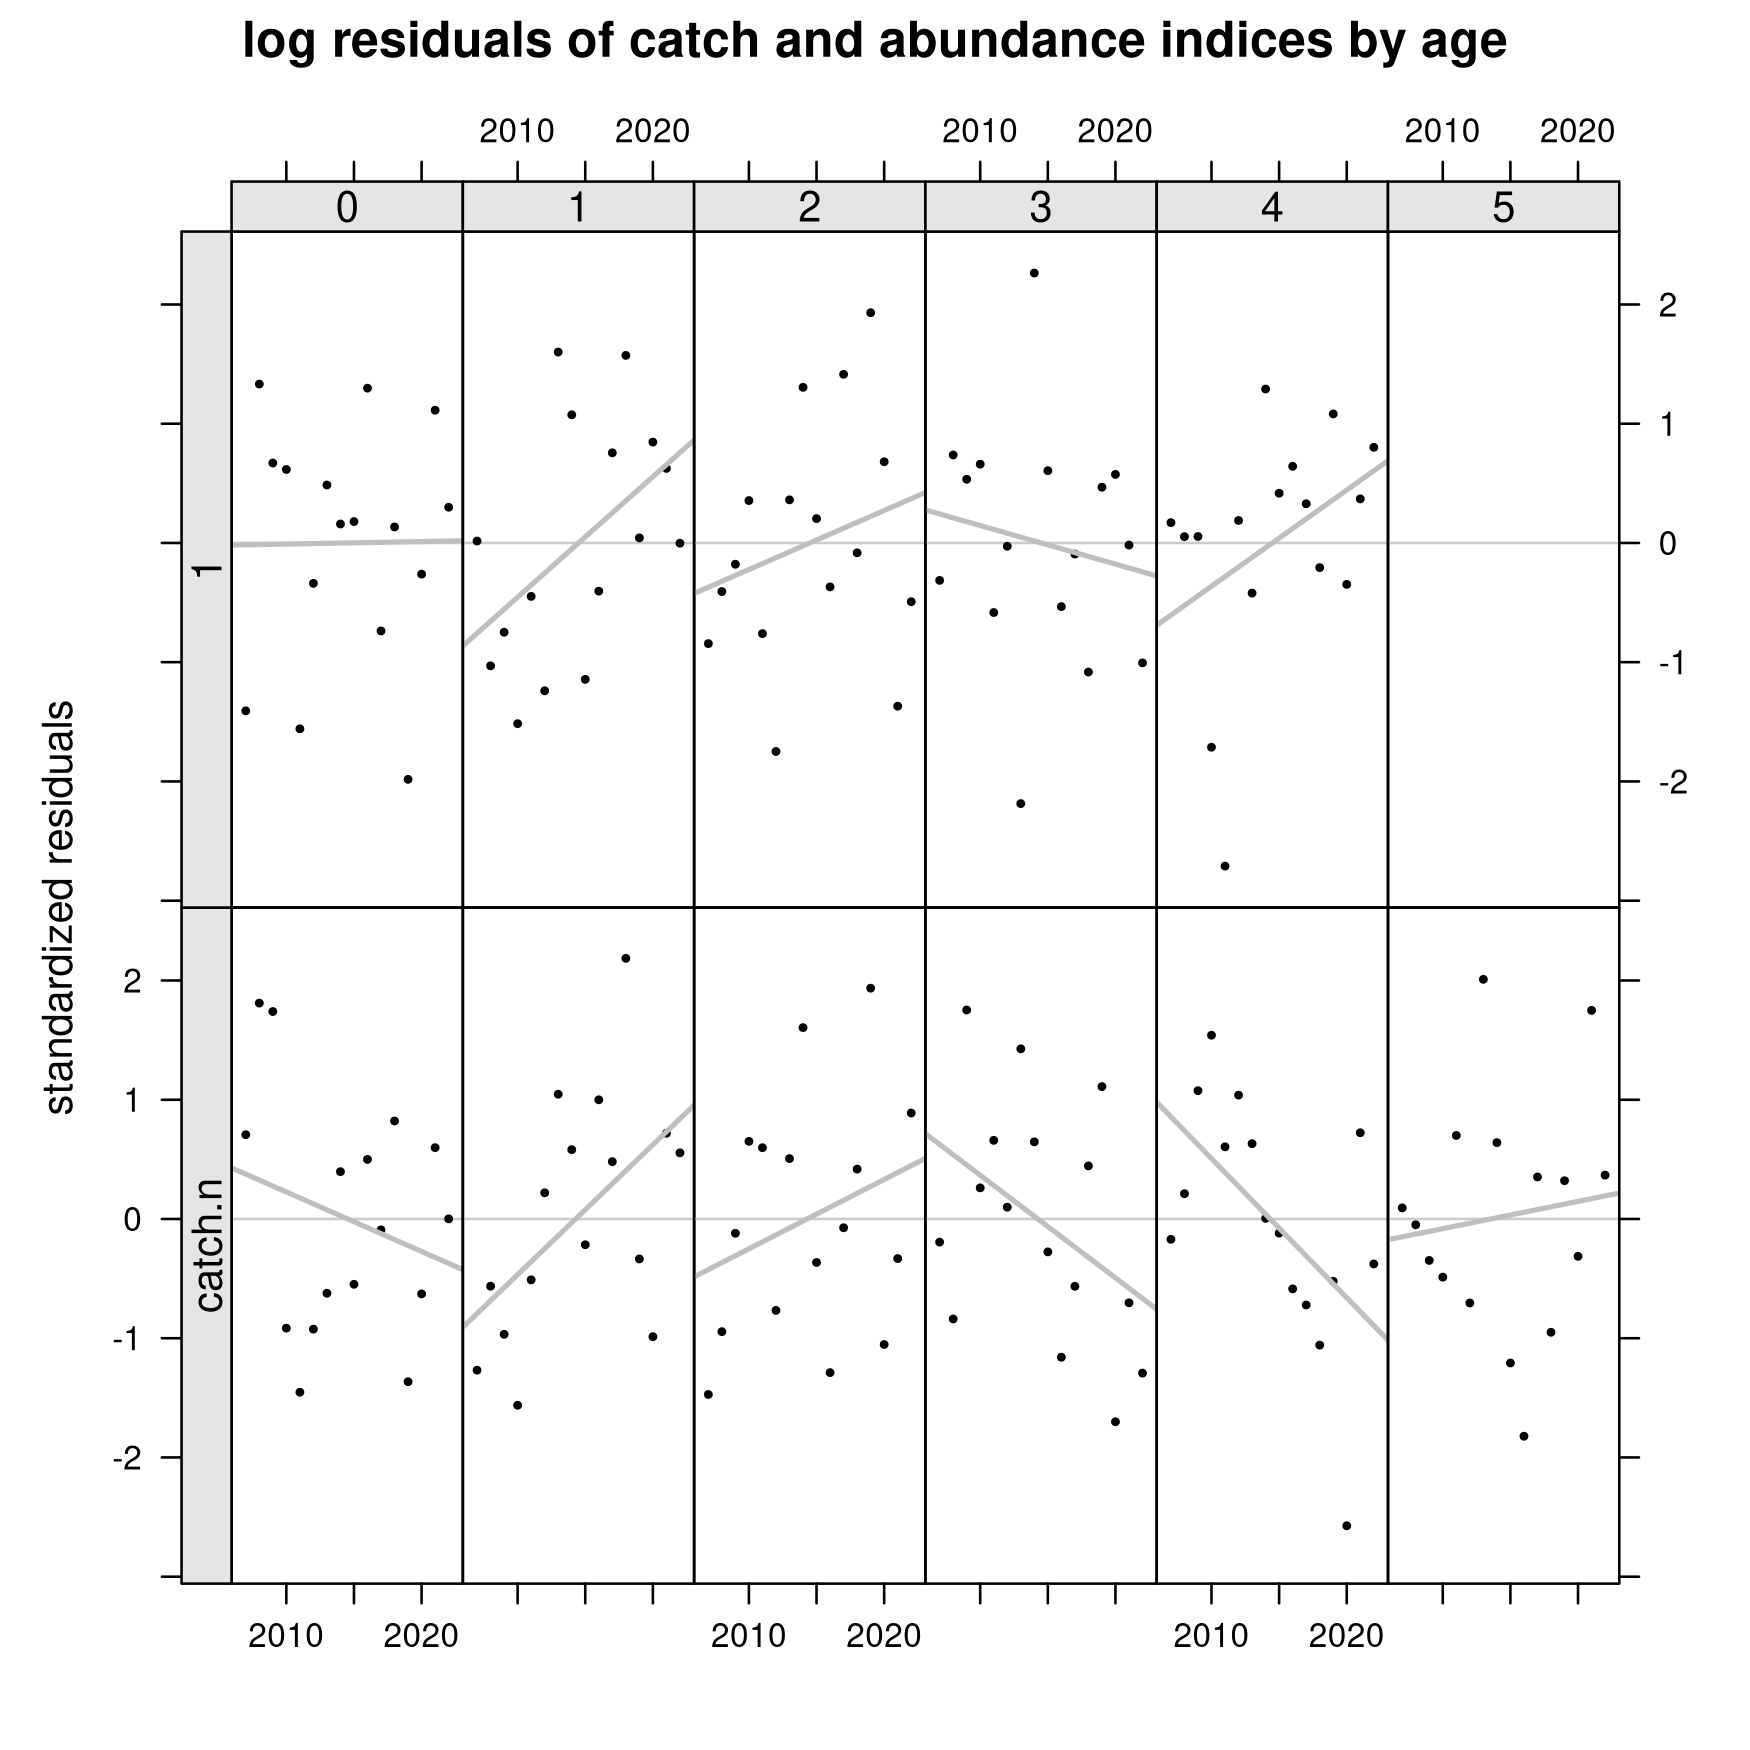
\includegraphics[width=.9\linewidth]{figure/srksresbyyear-1} 

}

\caption[f year effect fit residuals by year)]{f year effect fit residuals by year)}\label{fig:srksresbyyear}
\end{figure}

\end{knitrout}

\begin{knitrout}
\definecolor{shadecolor}{rgb}{0.949, 0.949, 0.949}\color{fgcolor}\begin{kframe}
\begin{alltt}
\hlkwd{plot}\hldef{(res09,} \hlkwc{auxline} \hldef{=} \hlsng{"l"}\hldef{,} \hlkwc{by} \hldef{=} \hlsng{"age"}\hldef{)}
\end{alltt}
\end{kframe}\begin{figure}[H]

{\centering 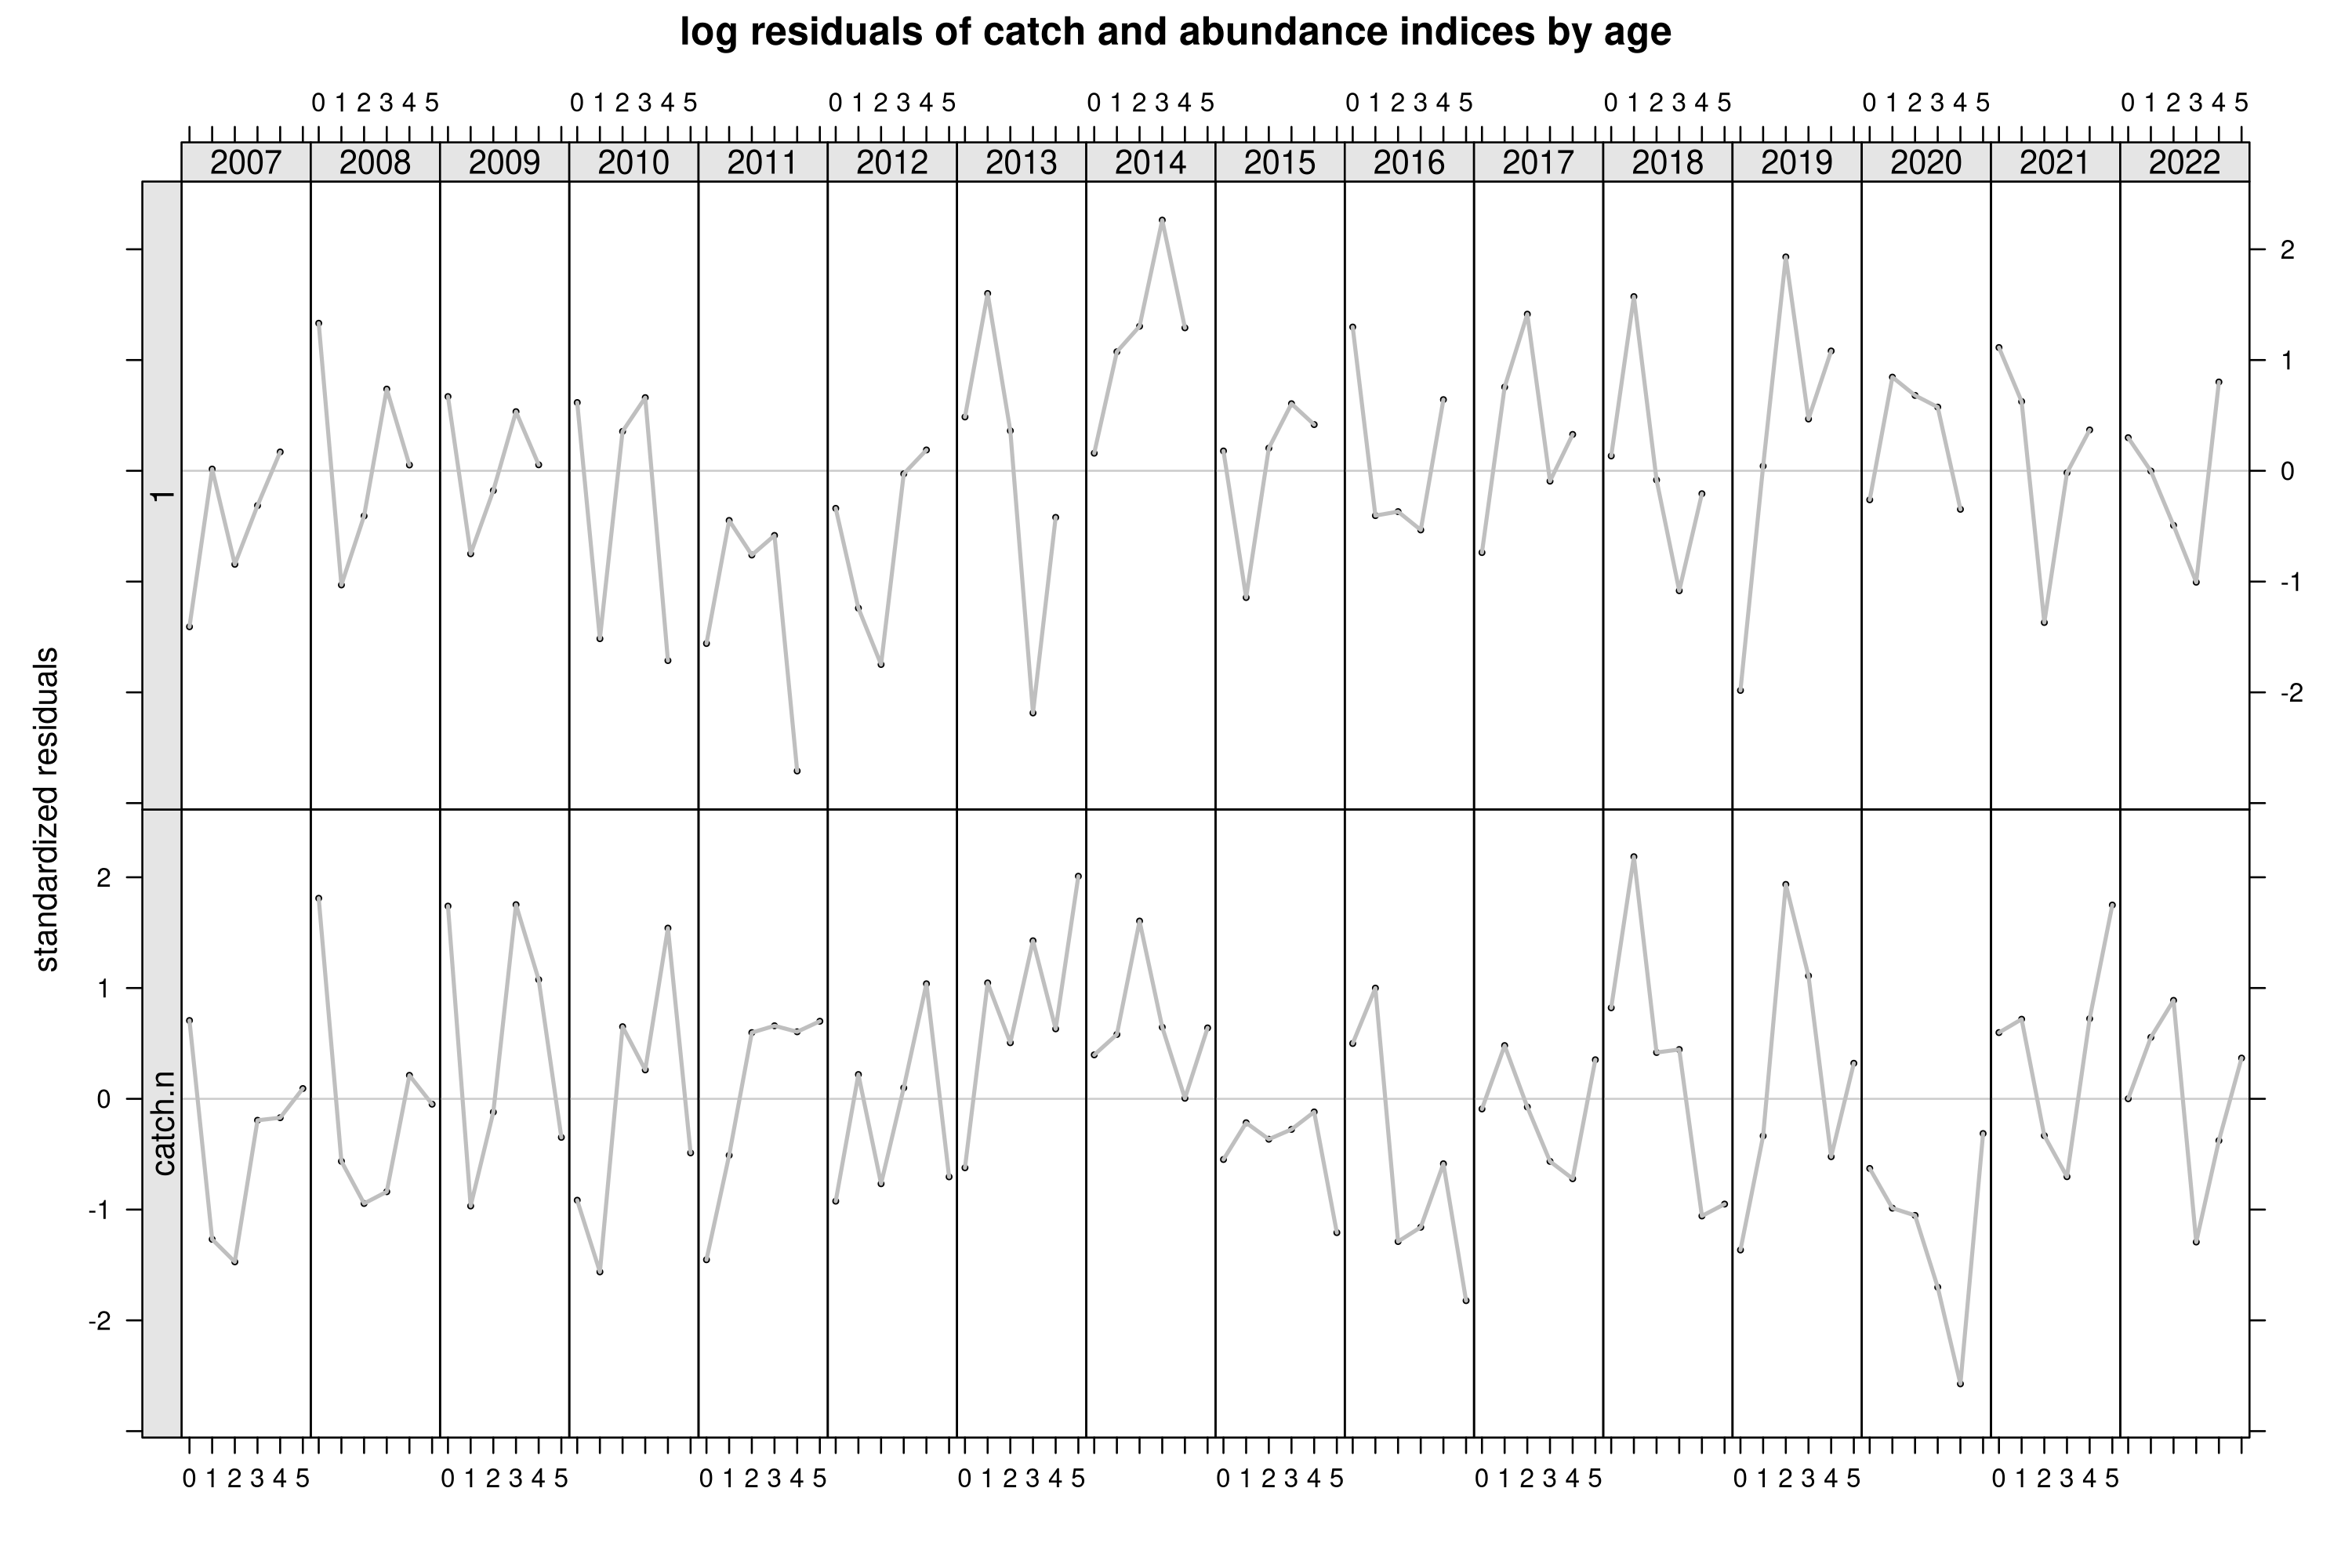
\includegraphics[width=25cm,height=18cm,angle=90]{figure/srksresbyage-1} 

}

\caption[f year effect fit residuals by age)]{f year effect fit residuals by age)}\label{fig:srksresbyage}
\end{figure}

\end{knitrout}

\subsection{The variance submodel}

Finally, we're testing the variance submodel, specifically the catch at age variance model. We won't dig into the catchability variance model though. It's common to accept that a scientific survey following a well designed sampling protocol will have equal variance across ages since no preferential areas are sampled. 

\begin{knitrout}
\definecolor{shadecolor}{rgb}{0.949, 0.949, 0.949}\color{fgcolor}\begin{kframe}
\begin{alltt}
\hldef{fit10} \hlkwb{<-} \hlkwd{sca}\hldef{(hke1567, hke1567.idx,} \hlkwc{fmod} \hldef{=} \hlopt{~}\hlkwd{factor}\hldef{(age)} \hlopt{+} \hlkwd{s}\hldef{(year,} \hlkwc{k} \hldef{=} \hlnum{5}\hldef{),} \hlkwc{qmod} \hldef{=} \hlkwd{list}\hldef{(}\hlopt{~}\hlkwd{factor}\hldef{(age)),}
    \hlkwc{srmod} \hldef{=} \hlopt{~}\hlkwd{s}\hldef{(year,} \hlkwc{k} \hldef{=} \hlnum{5}\hldef{),} \hlkwc{vmod} \hldef{=} \hlkwd{list}\hldef{(}\hlopt{~}\hlkwd{s}\hldef{(age,} \hlkwc{k} \hldef{=} \hlnum{4}\hldef{),} \hlopt{~}\hlnum{1}\hldef{),} \hlkwc{n1mod} \hldef{=} \hlopt{~}\hlkwd{factor}\hldef{(age))}
\hldef{res10} \hlkwb{<-} \hlkwd{residuals}\hldef{(fit10, hke1567, hke1567.idx)}
\end{alltt}
\end{kframe}
\end{knitrout}

To see what's happening with the variance model one can use predict to plot the different models fitted.

\begin{knitrout}
\definecolor{shadecolor}{rgb}{0.949, 0.949, 0.949}\color{fgcolor}\begin{kframe}
\begin{alltt}
\hldef{flqs} \hlkwb{<-} \hlkwd{FLQuants}\hldef{(}\hlkwc{mod10} \hldef{=} \hlkwd{predict}\hldef{(fit10)}\hlopt{$}\hldef{vmodel}\hlopt{$}\hldef{catch[,} \hlsng{"2017"}\hldef{],} \hlkwc{mod09} \hldef{=} \hlkwd{predict}\hldef{(fit09)}\hlopt{$}\hldef{vmodel}\hlopt{$}\hldef{catch[,}
    \hlsng{"2017"}\hldef{])}
\hlkwd{xyplot}\hldef{(data} \hlopt{~} \hldef{age,} \hlkwc{data} \hldef{= flqs,} \hlkwc{group} \hldef{= qname,} \hlkwc{type} \hldef{=} \hlsng{"l"}\hldef{,} \hlkwc{auto.key} \hldef{= T)}
\end{alltt}
\end{kframe}\begin{figure}[H]

{\centering 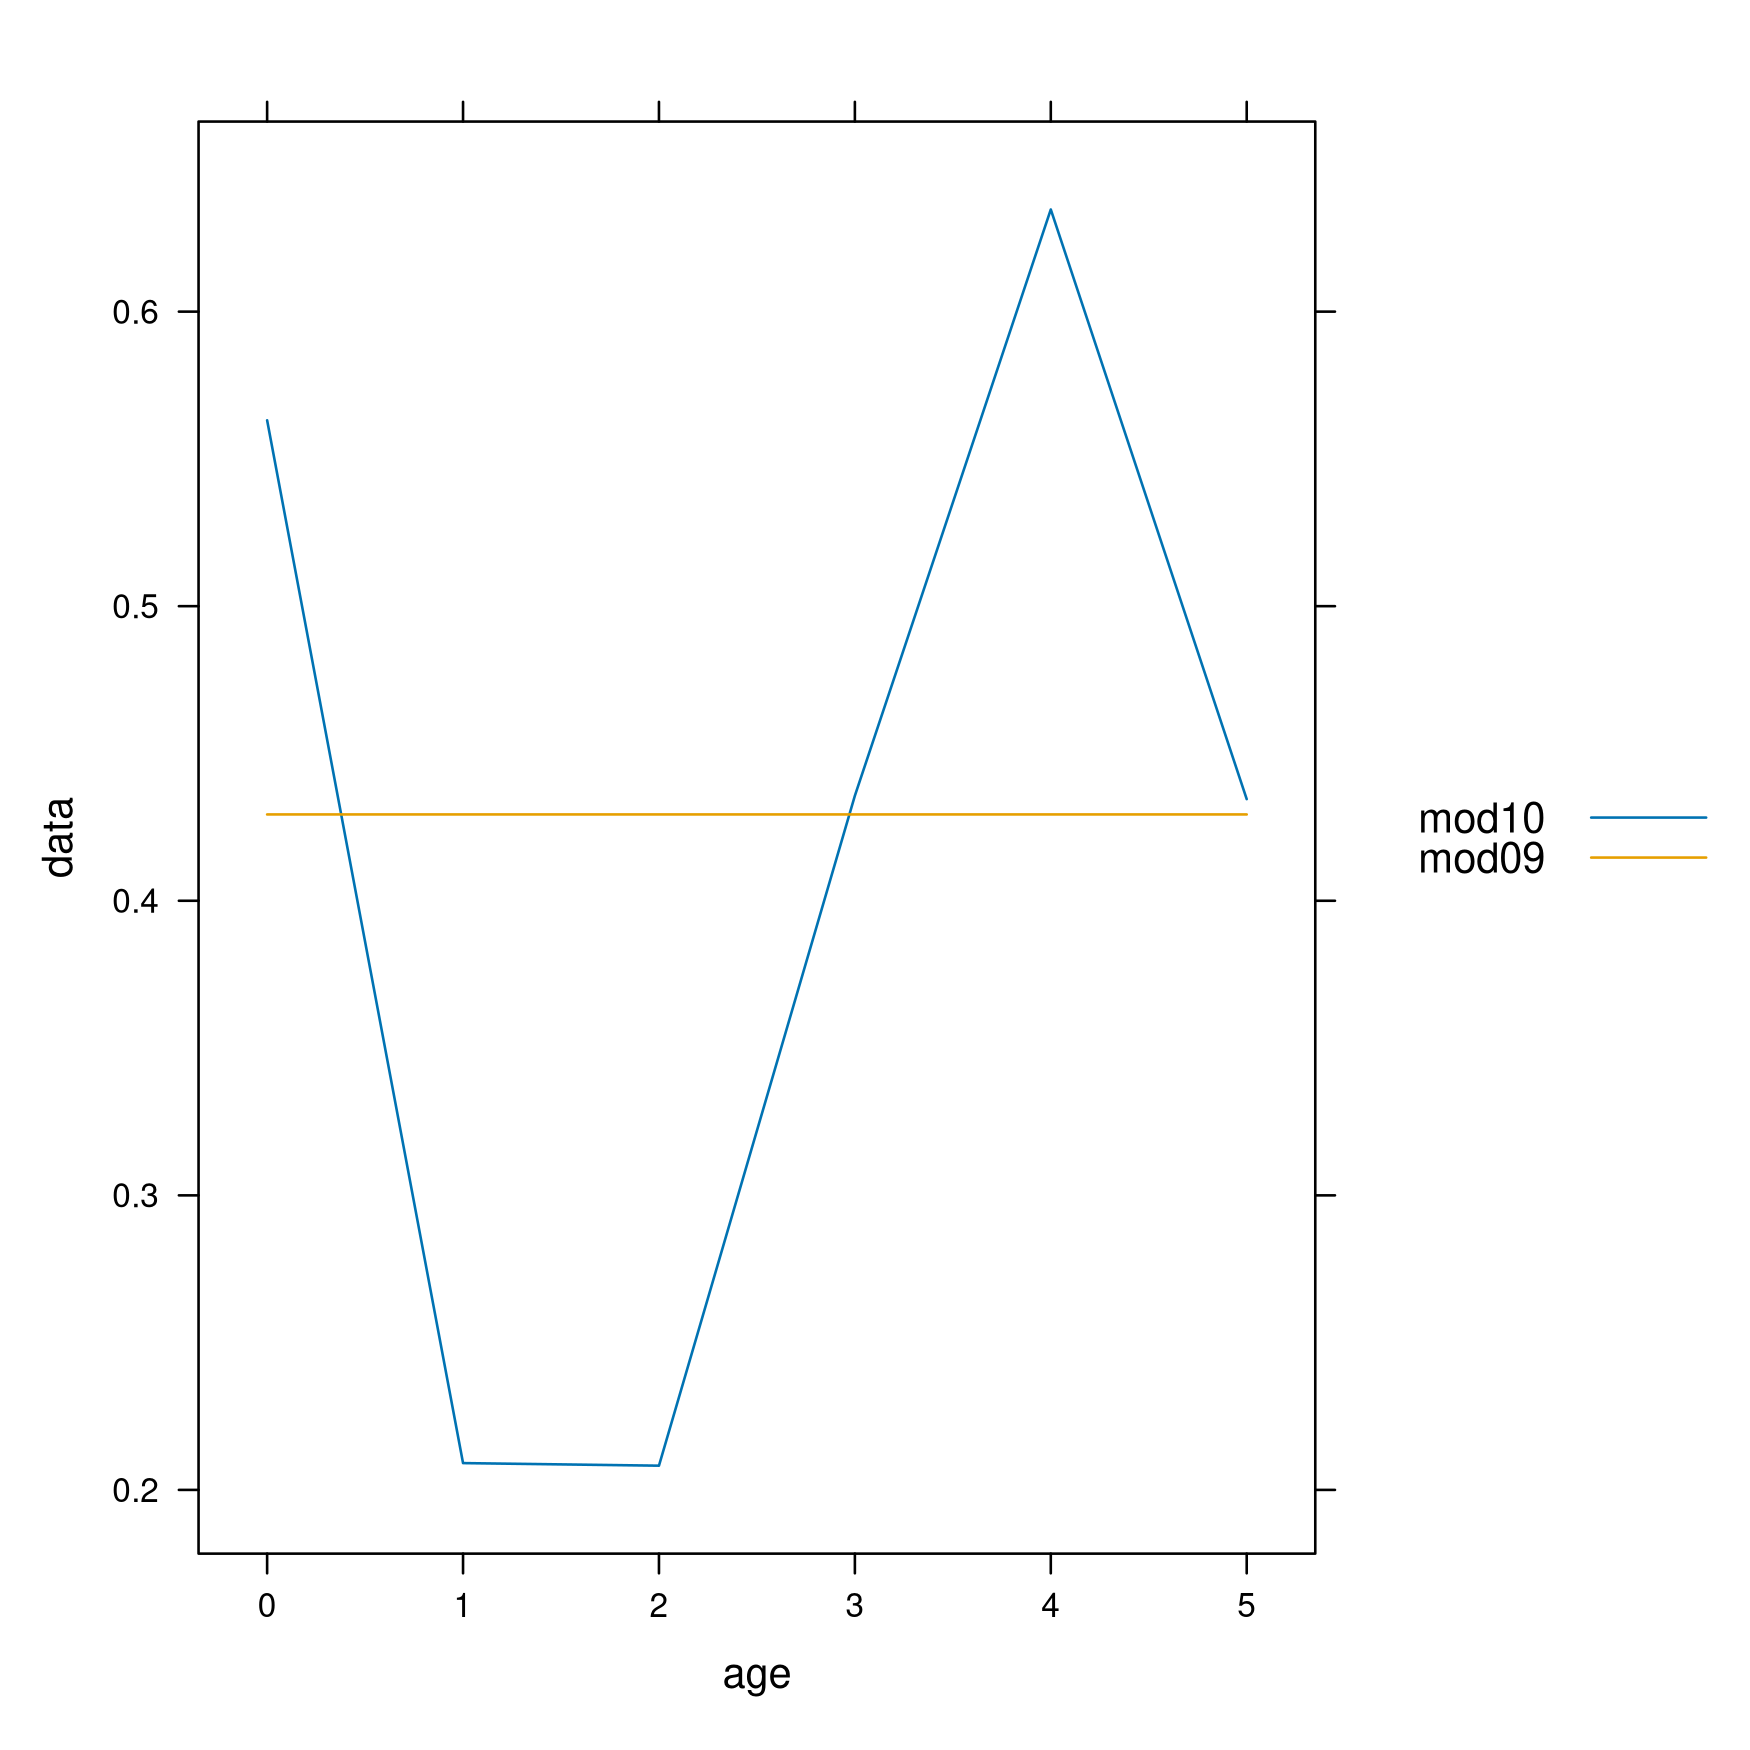
\includegraphics[width=.9\linewidth]{figure/vagepredbyage-1} 

}

\caption[Variance models for catch at age]{Variance models for catch at age}\label{fig:vagepredbyage}
\end{figure}

\end{knitrout}

To see the effect these models have on the estimated quantities one can look at the variance of the estimates:

\begin{knitrout}
\definecolor{shadecolor}{rgb}{0.949, 0.949, 0.949}\color{fgcolor}\begin{kframe}
\begin{alltt}
\hldef{flqs} \hlkwb{<-} \hlkwd{FLQuants}\hldef{(}\hlkwc{mod10} \hldef{=} \hlkwd{catch.n}\hldef{(hke1567} \hlopt{+} \hlkwd{simulate}\hldef{(fit10,} \hlkwc{nsim} \hldef{=} \hlnum{500}\hldef{))[,} \hlsng{"2017"}\hldef{],}
    \hlkwc{mod09} \hldef{=} \hlkwd{catch.n}\hldef{(hke1567} \hlopt{+} \hlkwd{simulate}\hldef{(fit09,} \hlkwc{nsim} \hldef{=} \hlnum{500}\hldef{))[,} \hlsng{"2017"}\hldef{])}
\hlkwd{bwplot}\hldef{(data} \hlopt{~} \hldef{qname} \hlopt{|} \hlkwd{factor}\hldef{(age),} \hlkwc{data} \hldef{=} \hlkwd{as.data.frame}\hldef{(flqs),} \hlkwc{scales} \hldef{=} \hlsng{"free"}\hldef{,} \hlkwc{auto.key} \hldef{= T)}
\end{alltt}
\end{kframe}\begin{figure}[H]

{\centering 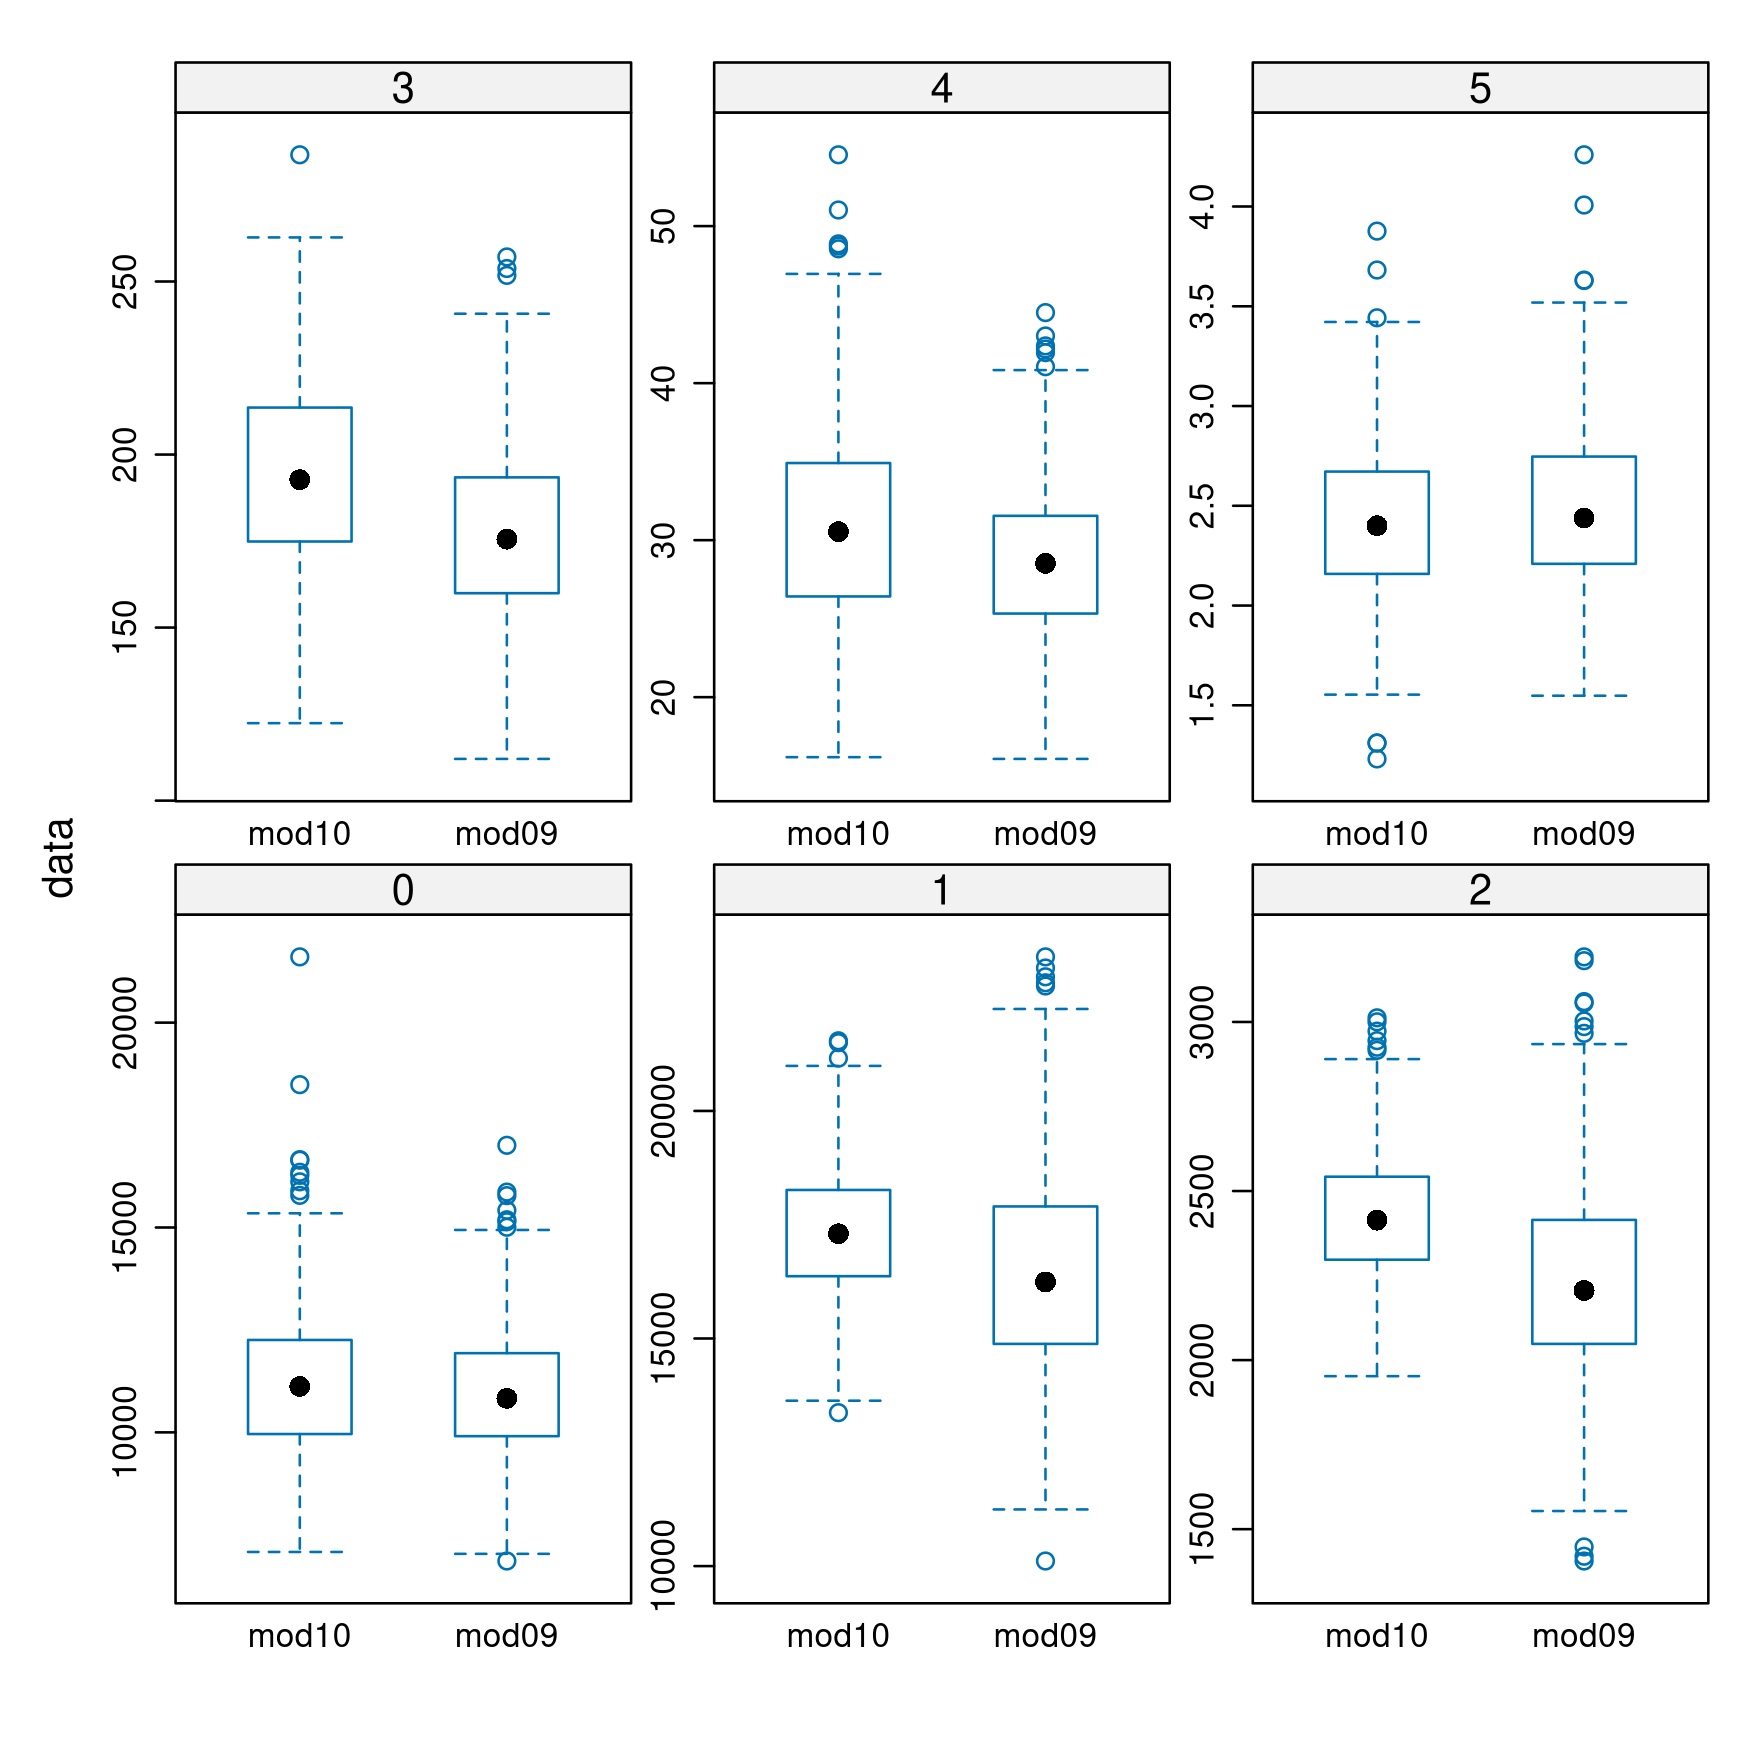
\includegraphics[width=.9\linewidth]{figure/vage-1} 

}

\caption[Estimates of population abundance with different variance models]{Estimates of population abundance with different variance models}\label{fig:vage}
\end{figure}

\end{knitrout}

and the usual residuals

\begin{knitrout}
\definecolor{shadecolor}{rgb}{0.949, 0.949, 0.949}\color{fgcolor}\begin{kframe}
\begin{alltt}
\hlkwd{plot}\hldef{(res10,} \hlkwc{auxline} \hldef{=} \hlsng{"r"}\hldef{)}
\end{alltt}
\end{kframe}\begin{figure}[H]

{\centering 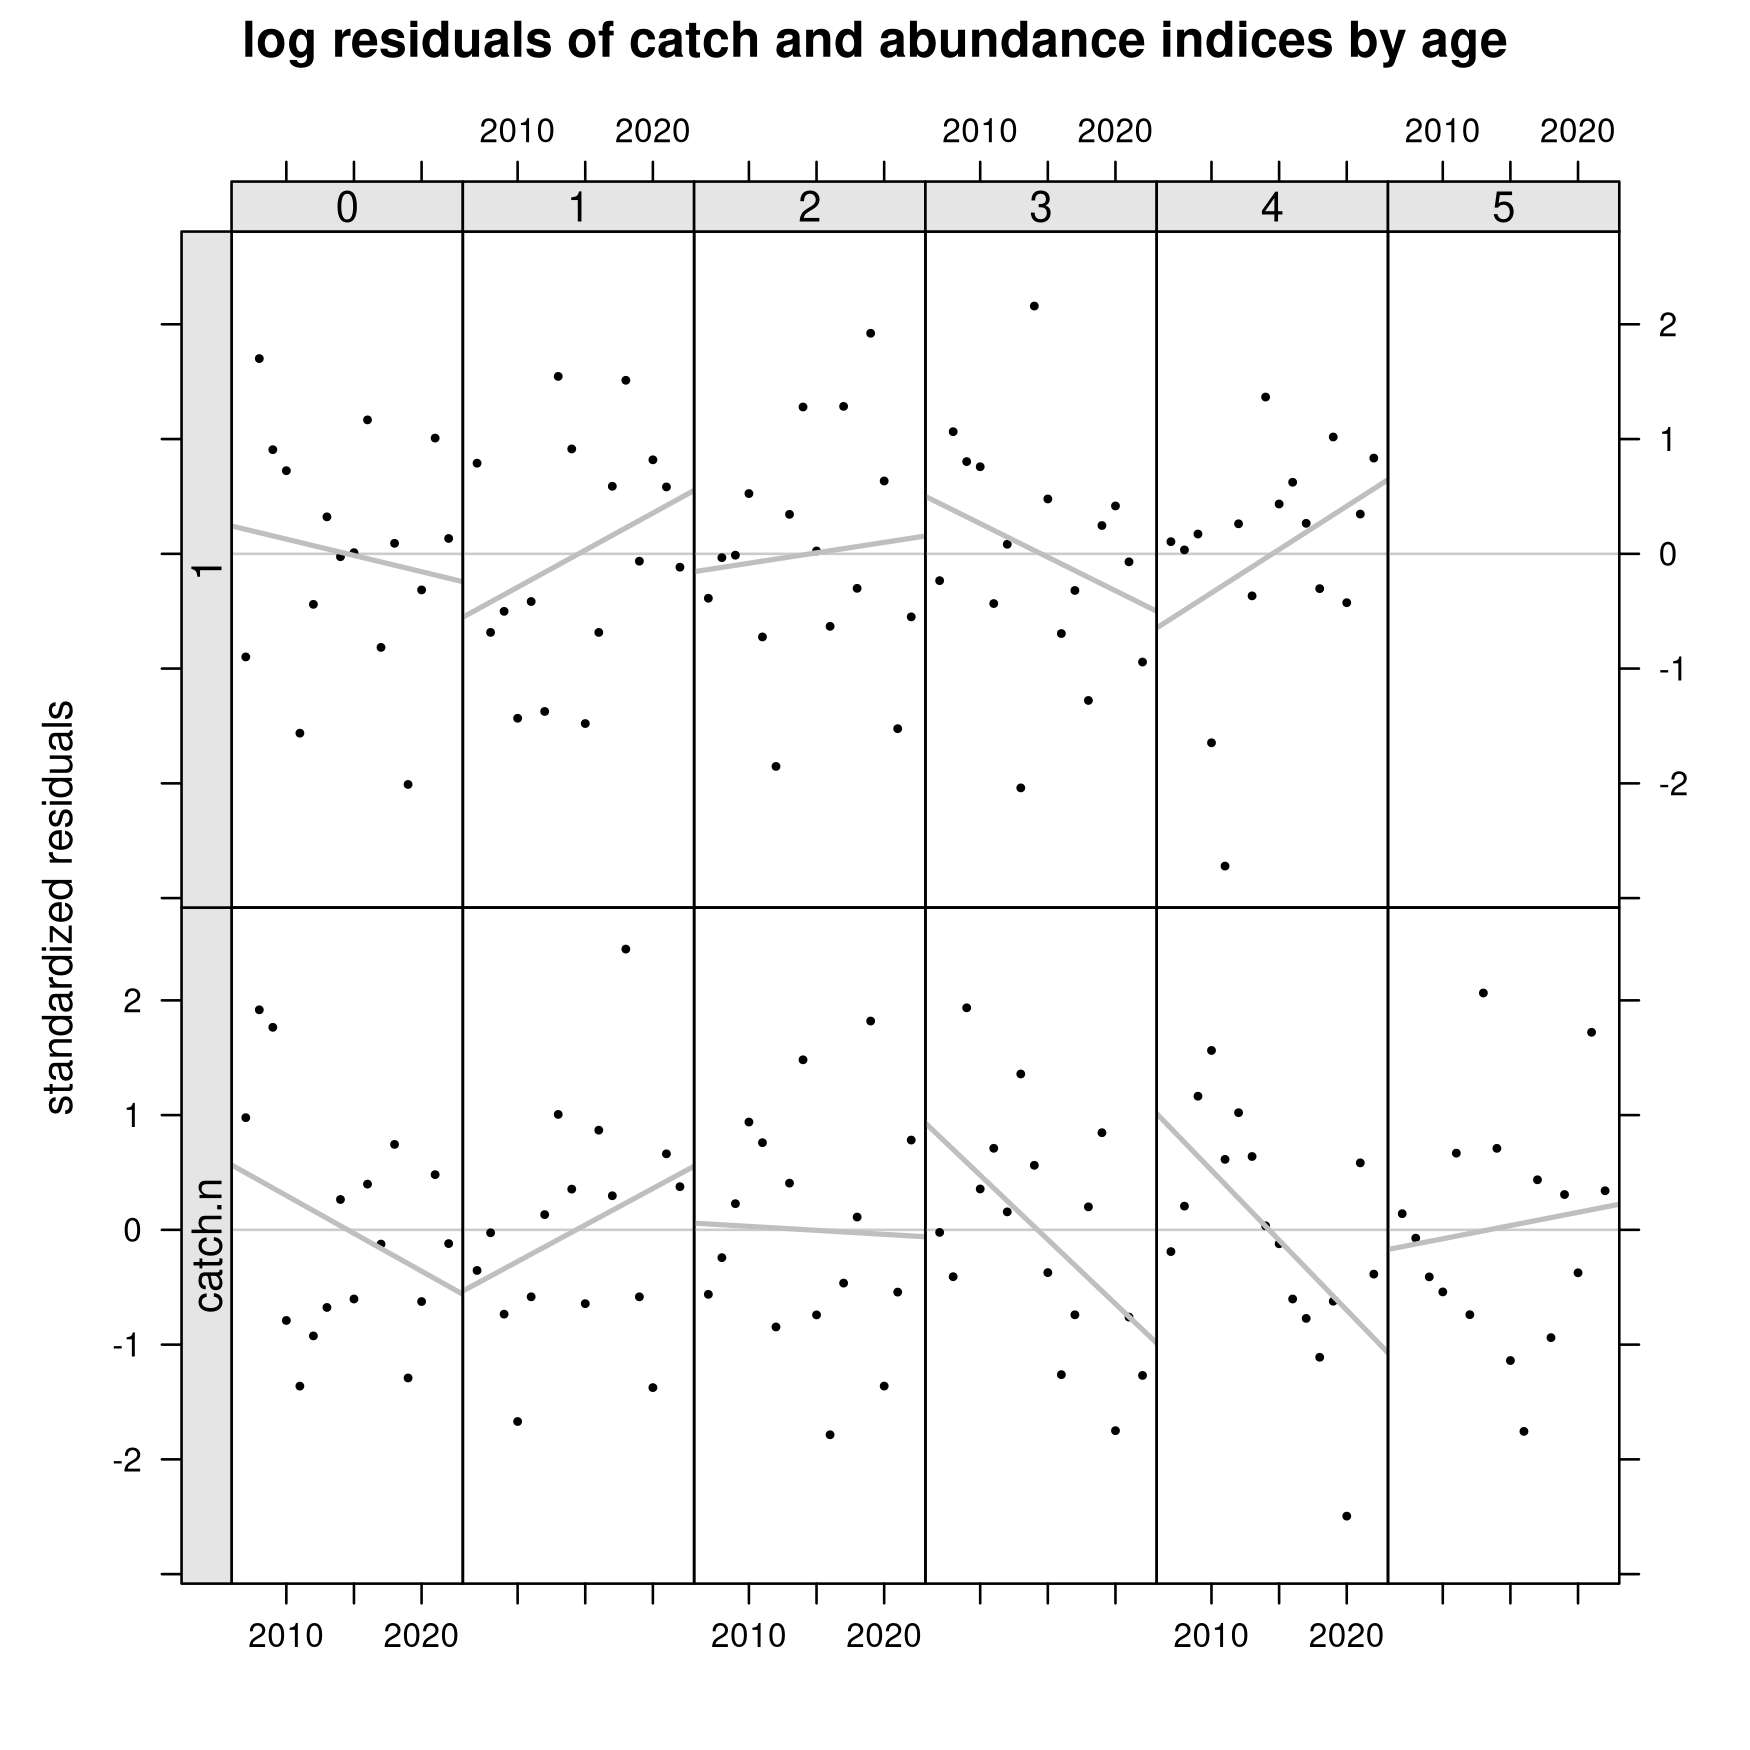
\includegraphics[width=.9\linewidth]{figure/vageresbyyear-1} 

}

\caption[f year effect fit residuals by year)]{f year effect fit residuals by year)}\label{fig:vageresbyyear}
\end{figure}

\end{knitrout}

\begin{knitrout}
\definecolor{shadecolor}{rgb}{0.949, 0.949, 0.949}\color{fgcolor}\begin{kframe}
\begin{alltt}
\hlkwd{plot}\hldef{(res10,} \hlkwc{auxline} \hldef{=} \hlsng{"l"}\hldef{,} \hlkwc{by} \hldef{=} \hlsng{"age"}\hldef{)}
\end{alltt}
\end{kframe}\begin{figure}[H]

{\centering 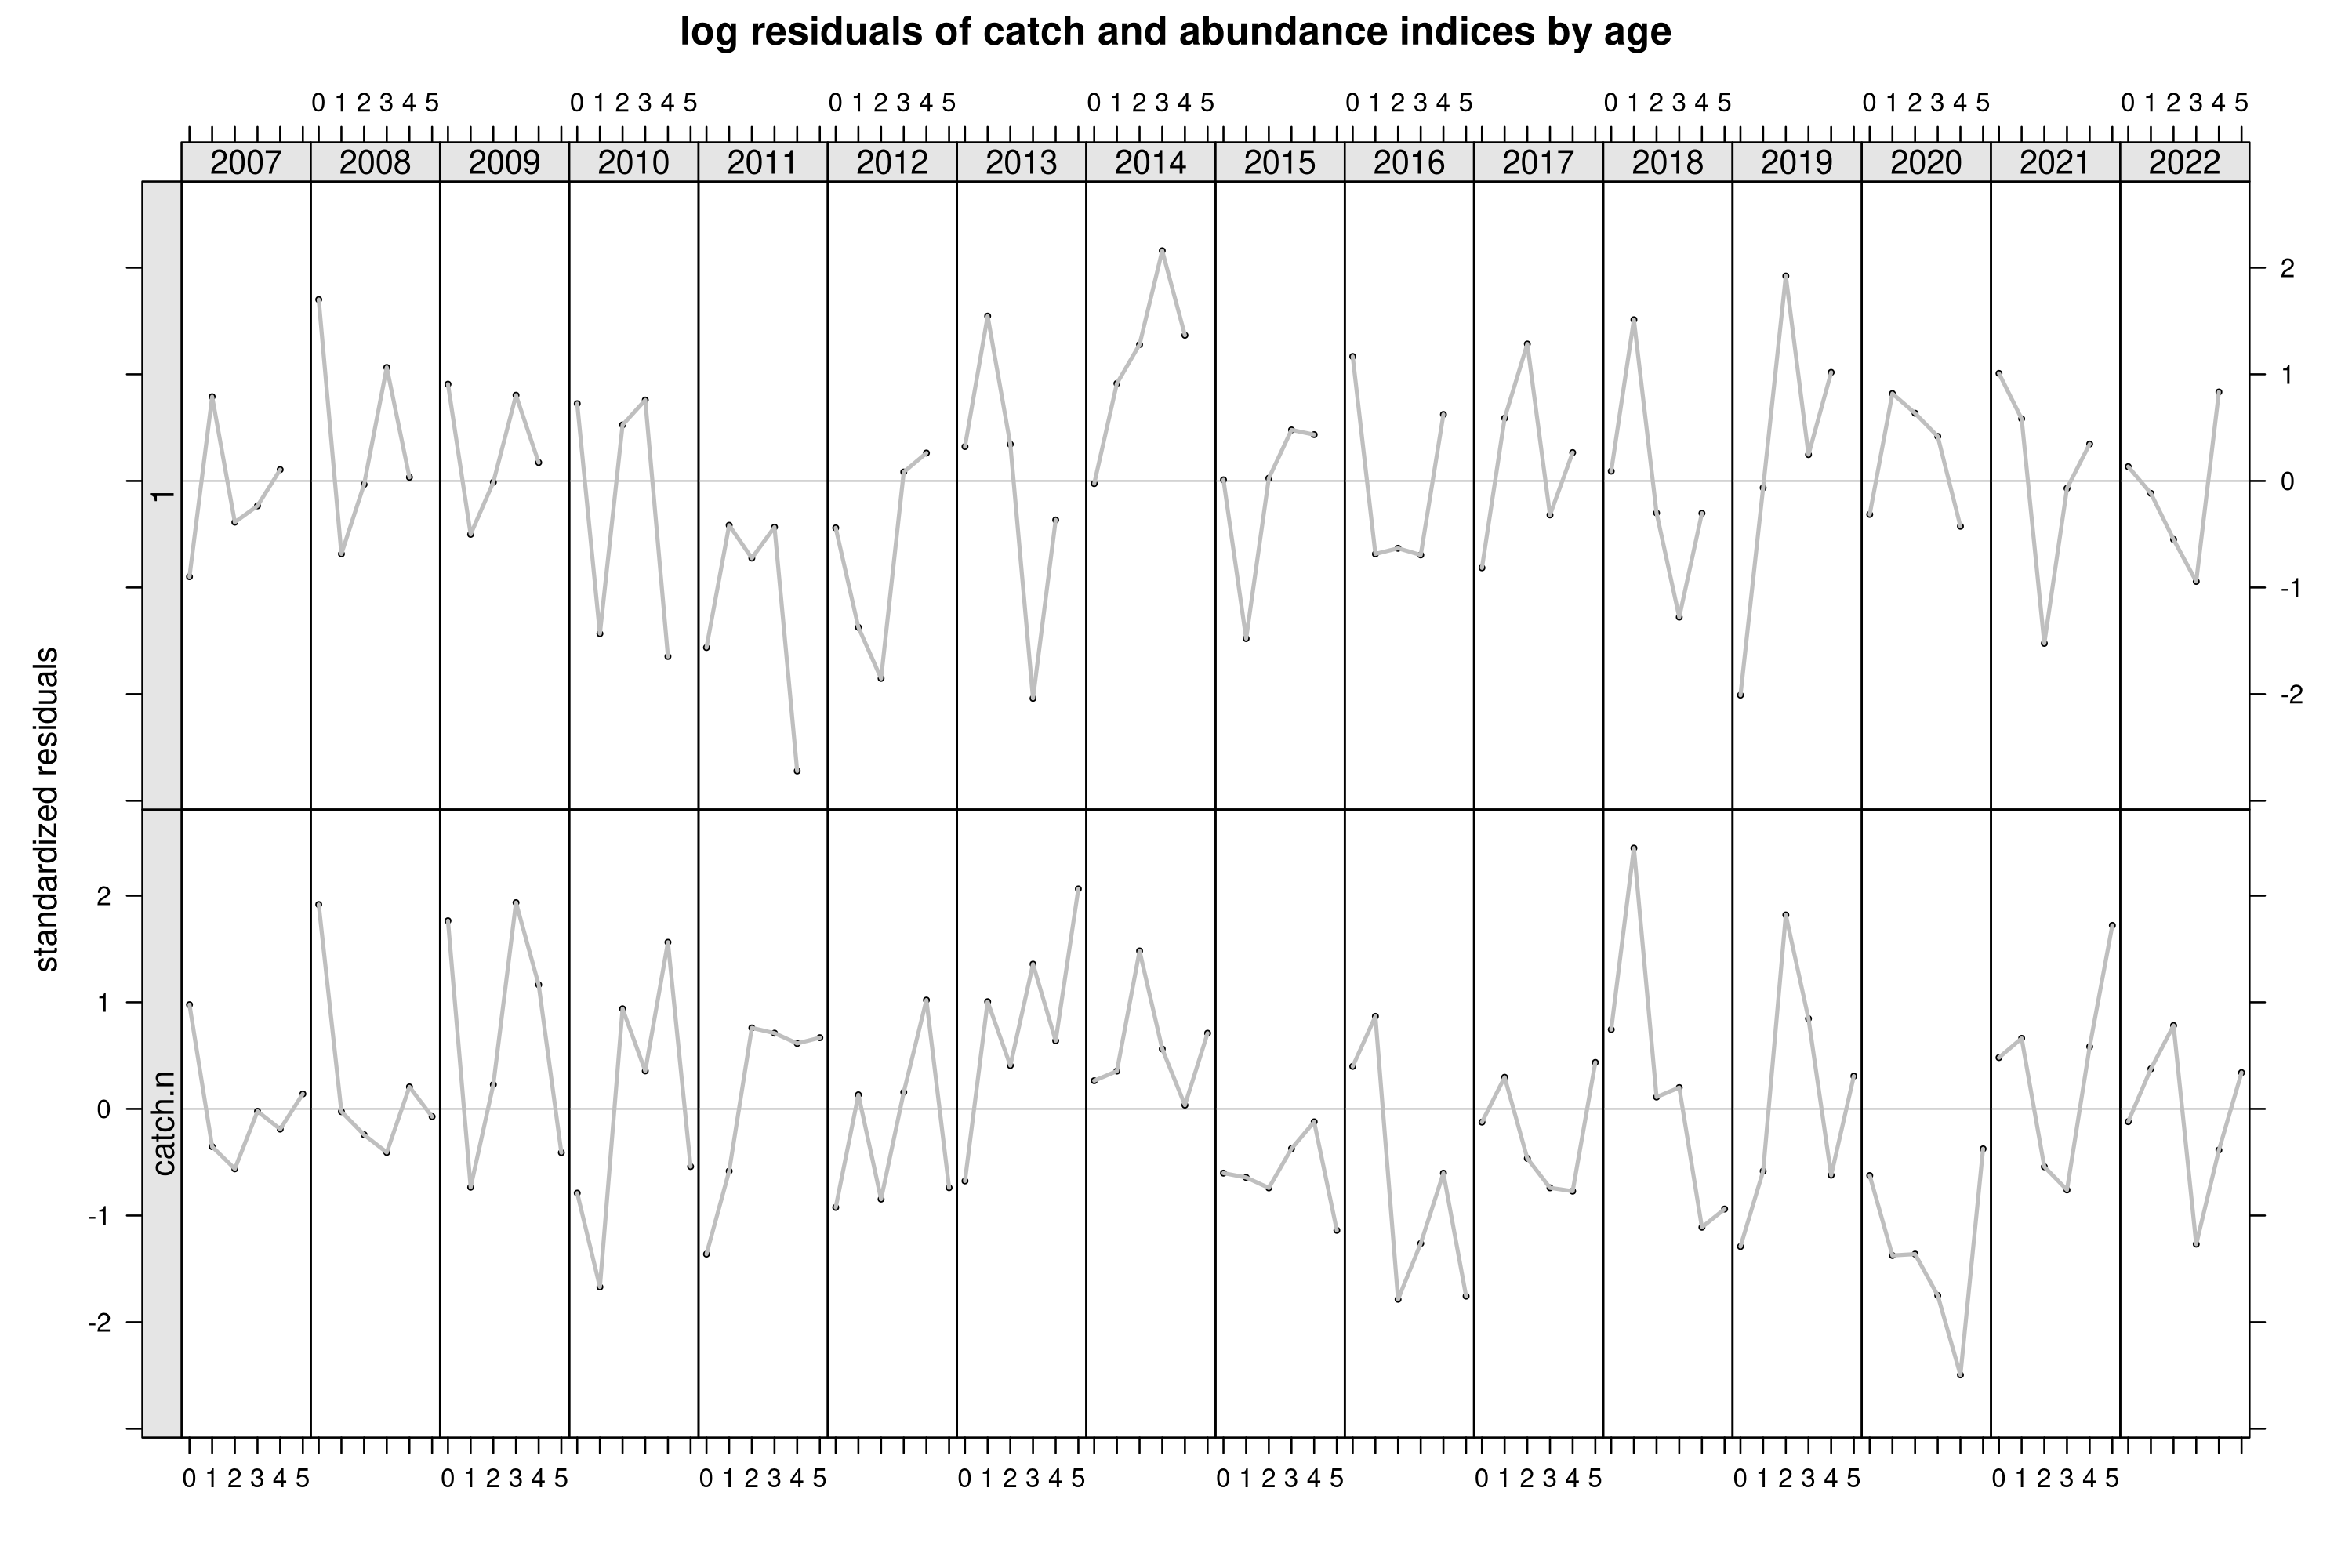
\includegraphics[width=25cm,height=18cm,angle=90]{figure/vageresbyage-1} 

}

\caption[f year effect fit residuals by age)]{f year effect fit residuals by age)}\label{fig:vageresbyage}
\end{figure}

\end{knitrout}

\end{document}
